 %\documentclass[1.5headlines,twoside, a4paper, 11pt, automark,final,headsepline]{scrreprt}
\documentclass[1.5headlines,twoside, openright, a4paper, 12pt, automark,final,headsepline, hidelinks]{scrbook}

%%****************
%% define medatata
%%________________
%\def\Title{An Example Document}
%\def\Author{Some Name}
%\def\Subject{An Example Document}
%\def\Keywords{LaTeX,Example,Document}
% 
%%***************************************************************************
%% \convertDate converts D:20080419103507+02'00' to 2008-04-19T10:35:07+02:00
%%___________________________________________________________________________
%\def\convertDate{%
%    \getYear
%}
% 
%{\catcode`\D=12
% \gdef\getYear D:#1#2#3#4{\edef\xYear{#1#2#3#4}\getMonth}
%}
%\def\getMonth#1#2{\edef\xMonth{#1#2}\getDay}
%\def\getDay#1#2{\edef\xDay{#1#2}\getHour}
%\def\getHour#1#2{\edef\xHour{#1#2}\getMin}
%\def\getMin#1#2{\edef\xMin{#1#2}\getSec}
%\def\getSec#1#2{\edef\xSec{#1#2}\getTZh}
%\def\getTZh +#1#2{\edef\xTZh{#1#2}\getTZm}
%\def\getTZm '#1#2'{%
%    \edef\xTZm{#1#2}%
%    \edef\convDate{\xYear-\xMonth-\xDay T\xHour:\xMin:\xSec+\xTZh:\xTZm}%
%}
% 
%\expandafter\convertDate\pdfcreationdate 
% 
%%**************************
%% get pdftex version string
%%__________________________
%\newcount\countA
%\countA=\pdftexversion
%\advance \countA by -100
%\def\pdftexVersionStr{pdfTeX-1.\the\countA.\pdftexrevision}
% 
% 
%%*********
%% XMP data
%\usepackage{xmpincl}
%
%
%\providecommand{\xmpAuthorURI}{} \providecommand{\xmpJournalnumber}{} \providecommand{\xmpVolume}{} \providecommand{\xmpIssue}{} \providecommand{\xmpCoverDisplayDate}{} \providecommand{\xmpCoverDate}{} \providecommand{\xmpJournaltitle}{} \providecommand{\xmpFirstpage}{} \providecommand{\xmpLastpage}{} \providecommand{\xmpDoi}{}
%
%
%\providecommand{\xmpProducer}{LaTeX2e}
%\providecommand{\xmpOrg}{MyOrg}
%\providecommand{\xmpTitle}{MyTitle}
%\providecommand{\xmpAuthor}{MyAuthor, mymail@gmail.com}
%\providecommand{\xmpKeywords}{MyKeywords}
%\providecommand{\xmpSubject}{MySubject}
%\providecommand{\xmpCreatorTool}{\pdftexbanner}
%\providecommand{\convDate}{\pdfcreationdate}
%\makeatletter
%
%\includexmp{pdfa-1b}
%\makeatother
% 
%%********
%% pdfInfo
%%________
%\pdfinfo{%
%    /Title    (\Title)
%    /Author   (\Author)
%    /Subject  (\Subject)
%    /Keywords (\Keywords)
%    /ModDate  (\pdfcreationdate)
%    /Trapped  /False
%}
%%****************************************
%% include the packages, commands and glossaries
\usepackage[a-1b]{pdfx}
\usepackage{xmpincl}
\usepackage[inner=3.0cm,outer=2cm,top=2cm,bottom=2cm,includeheadfoot]{geometry}
\usepackage[onehalfspacing]{setspace}
%\setstretch{baselinestretch}
%\linespread{1.5} % line spacing 
 
\usepackage[headsepline,plainheadsepline]{scrpage2}
\let\endgraph\endgraf        % necessary for "chapterprefix" in \documentclass call

% Header and footer definition
\clearscrheadfoot            % clear header and footer
\ohead[\headmark]{\headmark} % chapter names at top
\automark[section]{chapter}
\pagestyle{scrheadings}      % choose page style
%
%% % try to solve the width problem in PDF/A
%\usepackage[T1]{fontenc}

\ofoot[\pagemark]{\pagemark} % page number on the upper right side
%--------- separate abstract and content with one blank page---------- %
\usepackage{afterpage}
\newcommand\blankpage{%
    \null
    \thispagestyle{empty}%
    \addtocounter{page}{-1}%
    \newpage}
%\usepackage[backend=biber]{biblatex}
% ------ Language and Text Options
\usepackage[english]{babel}
\usepackage[latin9]{inputenc}
%\usepackage{pdflatex}
%\usepackage{color}
\usepackage{float}
%\usepackage{xmpincl}
\usepackage{hyperref}

%******** complexity O()*******
\usepackage{flushend}
\renewcommand{\O}[1]{$\mathcal{O}(#1)$}


%*********inline list
\usepackage{enumerate}
\usepackage[inline,shortlabels]{enumitem}

%%********inkscape to latex*************
%\usepackage{pstricks}
%%\usepackage{pst-plot}

%\usepackage[pdftex,
%        pdftoolbar=true, hyperfootnotes=false,breaklinks=true,
%        pdfpagelabels=true,
%        bookmarks, bookmarksopen, bookmarksnumbered, bookmarksopenlevel=1,
%        pdfauthor={Yanqiu Huang},
%        pdfsubject={Dissertation},%
%        pdfkeywords={WSNs, Energy efficiency, Data compression},
%        pdftitle={Dissertation,Yanqiu Huang,Uni-Bremen,2017},
%        pdfstartview={FitH},
%        pdfborder={0 0 0},  %Farbe aller Linkumrandung auf Wei� gesetzt
%        plainpages=false]{hyperref}
%\def\UrlBreaks{\do\/\do-}

% this package is used to remove the double printed math symbole problem
\usepackage{newtxtext,newtxmath}

\usepackage{etoc}
% ------ Math Packages
\usepackage{amsfonts}
\usepackage{amsmath}
\usepackage{bm}
%\usepackage{amssymb}
\newcommand\numberthis{\addtocounter{equation}{1}\tag{\theequation}}
%\usepackage{mathtools}
\usepackage[detect-none]{siunitx}
\usepackage[capitalize]{cleveref}
% ------ Source Code
\usepackage{listings}
%\usepackage{enumerate}
% ----- Floating Opjects
\usepackage{graphicx}
\usepackage{subfig}
\usepackage{xcolor}

%***packages for inputing the tikz pictures**********
\newlength\figureheight 
\newlength\figurewidth

\usepackage{pgfplots}
%******** change the tick, label size of the tikz figures********
\pgfplotsset{every axis/.append style={
		label style={font=\small},
		tick label style={font=\small}  
	}}
	
\usepackage{units}	
\usepackage{color}
	
\usepackage{epstopdf}
\usepackage{rotating}
\usepackage{multirow}		% -- multirow and multicolumn
\usepackage{booktabs}		% -- professional tables in LaTeX ,
\usepackage{longtable}
\usepackage{capt-of}
%\usepackage[bf]{caption}		% -- customise Captions
\usepackage{caption}		% -- customise Captions
\usepackage{placeins} 		% -- FloatBarrier
\usepackage{xspace}			% -- for a better layout of spaces
\usepackage{tabularx}

% ------ Table of Contents
\usepackage{minitoc}
%\dominitoc % for minitoc, default left-bounded
\setcounter{tocdepth}{2}
\setcounter{secnumdepth}{2}

% Packages for acronyms and list of symbols
%\usepackage{acronym}
\usepackage{makeidx}
\usepackage[section,style=alttree, sort=use]{glossaries}
\glssetwidest{ADCADCA}% widest name
\renewcommand*{\glsnamefont}[1]{\textmd{#1}}
\GlsSetQuote{+}
\usepackage{ifthen}

% *** SPECIALIZED LIST PACKAGES ***
\usepackage[flushleft]{threeparttable}
\usepackage[ruled, vlined, linesnumbered]{algorithm2e}
%\usepackage{algpseudocode}
%\usepackage[ruled,vlined,linesnumbered]{algorithm2e}
\usepackage{algorithmic}
\newtheorem{theorem}{Theorem}
\newenvironment{proof}[1][Proof]{\begin{trivlist}
\item[\hskip \labelsep {\bfseries #1}]}{\end{trivlist}}
%------ package for list of symbols
%\usepackage{glossaries}
\usepackage[]{appendix}		% -- include packages
% -- define your own commands
\newcommand\Fig[1]{\textbf{Fig.}~\ref{#1}}
\newcommand\fig[1]{\textbf{Fig.}~\ref{#1}}
\newcommand\Tab[1]{\textbf{Tab.}~\ref{#1}}
\newcommand\tab[1]{\textbf{Tab.}~\ref{#1}}
\newcommand\Equ[1]{\textbf{Eq.}~(\ref{#1})}
\newcommand\equ[1]{\textbf{Eq.}~(\ref{#1})}
\newcommand\Sect[1]{\textbf{Sec.}~\ref{#1}}
\newcommand\sect[1]{\textbf{Sec.}~\ref{#1}}
\newcommand\Refs[1]{\textbf{Ref.}~\cite{#1}}
\newcommand\refs[1]{\textbf{Ref.}~\cite{#1}}
\newcommand\Algo[1]{\textbf{Algorithm}~\ref{#1}}
\newcommand\algo[1]{\textbf{Algorithm}~\ref{#1}}
		% -- define your own commands
 %\clearpage
%\chapter{List of glossaries}
%\makeglossaries
%\makenoidxglossaries
%\printglossary
%\printnoidxglossary
%\newglossary*{acronym}{Acronym}
%\newglossary{acronym}{1i}{1o}{Acronym}
%\newacronym{wsn}{WSN}{wireless sensor network}
%\newacronym{pdf}{PDF}{probability density function}
\newacronym{cdf}{CDF}{Cumulative Density Function}
%\newacronym{mvn}{MVN}{multivariate normal}
%\newacronym{ridp}{Rand-idp}{Reconstruction solution using spatial and temporal correlation under random transmission}
\newcommand{\Axor}{A_\textnormal{{xor}}} % Size of a xor in math mode
\newcommand{\Aand}{A_\textnormal{{and}}} % Size of an and in math mode
\newcommand{\Amux}{A_\textnormal{{mux}}} % Size of an xor in math mode
\newcommand{\Aff}{A_\textnormal{{ff}}} % Size of an xor in math mode
\newcommand{\Txor}{T_\textnormal{{xor}}} % Size of a xor in math mode
\newcommand{\Tand}{T_\textnormal{{and}}} % Size of an and in math mode
\newcommand{\Tmux}{T_\textnormal{{mux}}} % Size of an xor in math mode
\newcommand{\ldceil}[1]{\lceil\log_2{\left({#1}\right)}\rceil}
\newcommand{\T}{{{S}}}
\newcommand{\cf}{{\delta}}
\newcommand{\PerM}{\mathbf{I}_\pi} % Definition of the Permutation matrix (I because der of Identity matrix)
\newcommand{\AssM}{\mathbf{I}_\sigma} % Definition of the assignment matrix (aus dem deutschen wikipedia "vozeichenbehaftete permutatiosnmatrix)
\newcommand{\AssOpt}{\mathbf{{I}_{\sigma,\textnormal{power-opt}}}} % Power-optimal assignment
\newcommand{\PerMCacOpt}{\mathbf{I}_{\pi,\textnormal{perf-opt}}}  % perf/CAC-opt assignment
\newcommand{\PerMTCOpt}{\mathbf{I}_{\pi,\textnormal{$\mathit{TC}$-opt}}} %Power+Perf.-opt assignment

% mean probability entry for the capacitance model
\newcommand{\meanP}{\bar{p}}

%----------------symbols------------------- %
\newglossary{math}{2i}{2o}{General mathematical symbols and specific operators}

%% \newglossaryentry{gf2}
%% { type=math, 
%%   name={\ensuremath{\mathbb{F}_2}},
%%   description={binary Galois field 2},
%%   %sort={F_2}
%% }

\newglossaryentry{log2}
{ type=math, 
	name={\ensuremath{\log_2(x)}},
	description={binary (base 2) logarithm of $x$},
	sort={log_2}
}




\newglossaryentry{bn}
{ type=math, 
	name={\ensuremath{\mathbb{N}}},
	description={set of  natural numbers: \{0,1,2,3,\dots \}},
	%sort={N}
}



%% \newglossaryentry{bb}
%% { type=math,
%%   name={\ensuremath{\mathbb{B}}},
%%   description={set of  binary numbers: \{0,1\}},
%%   %sort={B}
%% }

%% \newglossaryentry{bb_vec}
%% { type=math,
%%   name={\ensuremath{\mathbb{B}^n}},
%%   description={vector of $n$   binary numbers},
%%   %sort={B_n}
%% }

%% \newglossaryentry{bnm}
%% { type=math,
%%   name={\ensuremath{\mathbb{B}^{n\times m}}},
%%   description={matrix with $n$ rows and $m$ columns of binary numbers},
%%   %sort={B_nm}
%% }

%% \newglossaryentry{must_satisfy}
%% { type=math,
%%   name={\ensuremath{\stackrel{{ !}}{=}}},
%%   description={demanded equality},
%%   %sort={OPERATOR: demanded equality}
%% }



%% \newglossaryentry{defined}
%% { type=math,
%%   name={\ensuremath{\stackrel{{\textnormal{def}}}{=} }},
%%   description={defined as being equal to},
%%   %sort={OPERATOR: defined as being equal to}
%% }


%% \newglossaryentry{frobenius}
%% { type=math,
%%   name={\ensuremath{\langle \matr{M}_1, \matr{M}_2 \rangle }},
%%   description={Frobenius inner product of the matrices $\matr{M}_1$ and $\matr{M}_2$},
%%   %sort={OPERATOR: frobenius} 
%% }

%% \newglossaryentry{hadamard}
%% { type=math,
%%   name={\ensuremath{\matr{M}_1\circ \matr{M}_2}},
%%   description={Hadamard-product of the of  $\matr{M}_1$ and $\matr{M}_2$},
%%   %sort={OPERATOR: Hadamard}
%% }

\newglossaryentry{boolean_xor}
{ type=math,
	name={\ensuremath{\oplus}},
	description={Boolean \gls{xor} operator },
	%sort={OPERATOR: bit-wise boolean negation}
}


%% \newglossaryentry{max_matr}
%% { type=math, 
%%   name={\ensuremath{\max(\matr{M}_1, \matr{M}_2)}},
%%   description={maximum matrix of  $\matr{M}_1$ and $\matr{M}_2$ (entry-by-entry)},
%%   sort={F: maximum matrix}
%% }

%% \newglossaryentry{spark_matr}
%% { type=math, 
%%   name={\ensuremath{\spark(\matr{M})}},
%%   description={spark of a  matrix, \textit{i.e.,} the smallest integer $i$ such that there exists a set of $i$ columns of $\matr{M}$ that are linearly dependent.},
%%   sort={F: spark}
%% }




%% \newglossaryentry{proportional}
%% { type=math,
%%   name={\ensuremath{{\sim}}},
%%   description={proportionality},
%%   %sort={OA:Operator  proportionality}
%% }


%% \newglossaryentry{max_vector}
%% { type=math,
%%   name={\ensuremath{\max_{k,\,i}(\vec{V})}},
%%   description={maximum entry of a discrete-time vector, $\vec{V}$, over all cycles},
%%   sort={F: max vector} 
%% }


%% \newglossaryentry{maxdiag}
%% { type=math,
%%   name={\ensuremath{\maxdiag(\matr{M})}},
%%   description={maximum diagonal entry of  $\matr{M}$},
%%   sort={F: max diag}
%% }



%% \newglossaryentry{laplace_trans}
%% { type=math,
%%   name={\ensuremath{\mathcal{L}\{f(t)\}}},
%%   description={Laplace transform of $f(t)$},
%%   %sort={FUNCTION: Laplace transform}
%% }

\newglossaryentry{absolute_value}
{ type=math,
	name={\ensuremath{|X|}},
	description={the absolute value of variable $X$},
	%sort={FUNCTION: Operator Expectation}
}

\newglossaryentry{expected_value}
{ type=math,
	name={\ensuremath{\mathbb{E}\big[X\big]}},
	description={expectation operator for a value discrete variable $X$},
	%sort={FUNCTION: Operator Expectation}
}

\newglossaryentry{probability}
{ type=math,
	name={\ensuremath{Pr\big[x_i\big]}},
	description={probability of $x_i$ being 1},
	%sort={FUNCTION: Operator Expectation}
}

\newglossaryentry{average}
{ type=math,
	name={\ensuremath{\mu}},
	description={average error},
	%sort={$\sigma$}
}


\newglossaryentry{sigma}
{ type=math,
	name={\ensuremath{\sigma}},
	description={standard deviation of error},
	%sort={$\sigma$}
}

\newglossaryentry{variance}
{ type=math,
	name={\ensuremath{\sigma^2}},
	description={variance of error},
	%sort={$\sigma^2$}
}


\newglossaryentry{vdd}
{ type=math,
	name={\ensuremath{V_\textnormal{dd}}},
	description={power-supply voltage},
	%sort={v_dd}
}

\newglossaryentry{tclk}
{ type=math,
	name={\ensuremath{T_\textnormal{clk}}},
	description={period time of the clock determining the pattern duration},
	%sort={t_clk}
}

\newglossaryentry{fclk}
{ type=math,
	name={\ensuremath{f}},
	description={frequency equal to $\nicefrac{1}{T_\textnormal{clk}}$},
	%sort={f}
}


\newglossaryentry{tpd}
{ type=math,
	name={\ensuremath{T_\textnormal{pd}}},
	description={50\%--50\% propagation delay},
	%sort={t_pd}
}


% \newglossaryentry{expected_value_cont}
% { type=math,
%   name={\ensuremath{\mathbb{E}\{x\}}},
%   description={expectation operator for a value continuous variable $x$},
%   sort={OE:Operator Expectation Continuous}
% }



% --------------physical parameters--------------- %
%\newglossary{geometrics}{2i}{2o}{Defined Symbols}



% \newglossaryentry{Ee}
% { type=symbols,
%   name={\ensuremath{E_{\textnormal{e},i}}},
%   description={extracted  energy from the driver of the $i^\textnormal{th}$ interconnect},
%   sort={P:Clock-period}
% }

% \newglossaryentry{Ee}
% { type=symbols,
%   name={\ensuremath{i_{i}}},
%   description={extracted  energy from the driver of the $i^\textnormal{th}$ interconnect},
%   sort={P:Clock-period}
% }





%----------------symbols high level power and perforamance------------------- %
%\newglossary{symbol}{2i}{2o}{Defined Symbols used in Multiple Chapters}

%% \newglossaryentry{wl}
%% { type=symbol,
%%   name={\ensuremath{\nicefrac{W}{L_\textnormal{min}}}},
%%   description={width-over-minimum-length ratio of a transistor},
%%   sort=WL
%% }

%% \newglossaryentry{rho}
%% { type=symbol, 
%%   name={\ensuremath{\rho}},
%%   description={Word-level correlation of the data},
%%   sort={$\rho$}
%% }


%% \newglossaryentry{rtsv}
%% { type=symbol,
%%   name={\ensuremath{r_\textnormal{tsv}}},
%%   description={\acrshort{tsv} radius},
%%   sort={r_tsv}
%% }


%% \newglossaryentry{mxn}
%% { type=symbol,
%%   name={\ensuremath{M \times N}},
%%   description={row and column count of the \acrshort{tsv} array},
%%   sort={MxN}
%% }


%% \newglossaryentry{tox}
%% { type=symbol,
%%   name={\ensuremath{t_\textnormal{ox}}},
%%   description={\acrshort{tsv} oxide thickness},
%%   sort={t_ox}
%% }

%% \newglossaryentry{wdep}
%% { type=symbol,
%%   name={\ensuremath{w_{\textnormal{dep},i}}},
%%   description={depletion-region width for \acrshort{tsv} $i$},
%%   sort={w_dep}
%% }


%% \newglossaryentry{dmin}
%% { type=symbol,
%%   name={\ensuremath{d_\textnormal{min}}},
%%   description={minimum \acrshort{tsv} pitch},
%%   sort={d_min}
%% }

%% \newglossaryentry{ltsv}
%% { type=symbol,
%%   name={\ensuremath{l_\textnormal{tsv}}},
%%   description={through-silicon-via length/depth},
%%   sort={l_tsv}
%% }


%% \newglossaryentry{vdd}
%% { type=symbol,
%%   name={\ensuremath{V_\textnormal{dd}}},
%%   description={power-supply voltage},
%%   sort={v_dd}
%% }

%% \newglossaryentry{tclk}
%% { type=symbol,
%%   name={\ensuremath{T_\textnormal{clk}}},
%%   description={period time of the clock determining the pattern duration},
%%   sort={t_clk}
%% }

%% \newglossaryentry{fclk}
%% { type=symbol,
%%   name={\ensuremath{f}},
%%   description={frequency equal to $\nicefrac{1}{T_\textnormal{clk}}$},
%%   sort={f}
%% }

%% \newglossaryentry{c_ij}
%% { type=symbol,
%%   name={\ensuremath{C_{i,j}}},
%%   description={coupling capacitance between interconnect $i$ and $j$ for $i\neq j$; self/ground capacitance of interconnect $i$ for $i=j$},
%%     sort={c_ij}
%% }

%% \newglossaryentry{P}
%% { type=symbol,
%%   name={\ensuremath{P}},
%%   description={interconnect power consumption},
%%   sort={P}
%% }

%% \newglossaryentry{tpd}
%% { type=symbol,
%%   name={\ensuremath{T_\textnormal{pd}}},
%%   description={interconnect 50\%--50\% propagation delay},
%%   sort={t_pd}
%% }


%% \newglossaryentry{fs}
%% { type=symbol,
%%   name={\ensuremath{f_\textnormal{s}}},
%%   description={significant frequency of the \acrshort{tsv} signals},
%%   sort={f_s}
%% }


%% \newglossaryentry{binary_signal}
%% { type=symbol,
%%   name={\ensuremath{b_{i}}},
%%   description={clock-cycle based bit signal ($b_i \in \mathbb{B}$)},
%%   sort={b_i}
%% }

%% \newglossaryentry{binary_signal_switch}
%% { type=symbol,
%%   name={\ensuremath{\Delta b_{i}}},
%%   description={clock-cycle based switching of $b_i$ ($\Delta b_i$  $\in \{-1,0,1\}$)},
%%   sort={$\Delta$ b_i}
%% }


% \newglossaryentry{misalignment}
% { type=symbol,
%   name={\ensuremath{T_{\textnormal{skew},i,j}}},
%   description={temporal misalignment/skew between the switching times of two binary signals $b_i$ and $ b_j$},
%   sort={T_skew}
%}

%% \newglossaryentry{edge_delay}
%% { type=symbol,
%%   name={\ensuremath{T_{\textnormal{edge},i}}},
%%   description={delay on the signal edges on $b_i$ compared to the rising clock edge},
%%   sort={T_edge}
%% }



%% \newglossaryentry{effective_capacitance}
%% { type=symbol,
%%   name={\ensuremath{C_{\textnormal{eff},i}}},
%%   description={clock-cycle-based effective capacitance  for interconnect $i$},
%%   sort={c_eff}
%% }


%% \newglossaryentry{mean_effective_capacitance}
%% { type=symbol,
%%   name={\ensuremath{\bar{C}_{\textnormal{eff},i}}},
%%   description={mean effective capacitance  for interconnect $i$},
%%   sort={c_eff_mean}
%% }

% \newglossaryentry{hat_effective_capacitance_single}
% { type=symbol,
%   name={\ensuremath{\hat{C}_{\textnormal{eff},i}}},
%   description={maximum possible effective capacitance  for interconnect $i$},
%   sort={c_eff_max}
% }

%% \newglossaryentry{hat_effective_capacitance}
%% { type=symbol,
%%   name={\ensuremath{\hat{C}_{\textnormal{eff}}}},
%%   description={maximum possible effective capacitance  for all interconnects},
%%   sort={c_eff_max2}
%% }





%% \newglossaryentry{coup_capacitance_mw}
%% { type=symbol,
%%   name={\ensuremath{{C}_{\textnormal{mw,c}}}},
%%   description={capacitance of adjacent metal wires },
%%   sort={c_mw_c}
%% }


%% \newglossaryentry{ground_capacitance_mw}
%% { type=symbol,
%%   name={\ensuremath{{C}_{\textnormal{mw,g}}}},
%%   description={ground capacitance of a metal wire},
%%   sort={c_mw_g}
%% }

%% \newglossaryentry{coup_capacitance_tsv}
%% { type=symbol,
%%   name={\ensuremath{{C}_{\textnormal{n}}}},
%%   description={coupling capacitance of  direct adjacent middle \acrshortpl{tsv}},
%%   sort={c_n}
%% }


%% \newglossaryentry{coup_capacitance_tsv_diag}
%% { type=symbol,
%%   name={\ensuremath{{C}_{\textnormal{d}}}},
%%   description={coupling capacitance of diagonal adjacent \acrshortpl{tsv}},
%%   sort={c_d}
%% }


%% \newglossaryentry{self_capacitance_tsv_edge}
%% { type=symbol,
%%   name={\ensuremath{{C}_{\textnormal{e0}}}},
%%   description={ground capacitance of an edge \acrshort{tsv} located not at a corner},
%%   sort={c_e0}
%% }


%% \newglossaryentry{coupling_capacitance_tsv_edge}
%% { type=symbol,
%%   name={\ensuremath{{C}_{\textnormal{e1}}}},
%%   description={coupling capacitance of two direct adjacent edge \acrshortpl{tsv} located not at a corner},
%%   sort={c_e1}
%% }

%% \newglossaryentry{coupling_capacitance_tsv_edge2}
%% { type=symbol,
%%   name={\ensuremath{{C}_{\textnormal{e2}}}},
%%   description={coupling capacitance of two indirect adjacent edge \acrshort{tsv} located not at a corner},
%%   sort={c_e2}
%% }


%% \newglossaryentry{self_capacitance_tsv_corner}
%% { type=symbol,
%%   name={\ensuremath{{C}_{\textnormal{c0}}}},
%%   description={ground capacitance of a corner \acrshort{tsv}},
%%   sort={c_c0}
%% }


%% \newglossaryentry{coupling_capacitance_tsv_corner}
%% { type=symbol,
%%   name={\ensuremath{{C}_{\textnormal{c1}}}},
%%   description={coupling capacitance of a corner \acrshort{tsv} and  a direct adjacent  \acrshort{tsv}},
%%   sort={c_c1}
%% }

%% \newglossaryentry{coupling_capacitance_tsv_corner2}
%% { type=symbol,
%%   name={\ensuremath{{C}_{\textnormal{c2}}}},
%%   description={coupling capacitance of a corner \acrshort{tsv} and  an indirect adjacent  \acrshort{tsv}},
%%   sort={c_c2}
%% }

%% \newglossaryentry{p_i}
%% { type=symbol,
%%   name={\ensuremath{p_{i}}},
%%   description={probability of the  $b_i$  being 1 ($\mathbb{E}\{b_i\}$)},
%%   sort={p_i}
%% }
% \newglossaryentry{p_ij}
% { type=symbol,
%   name={\ensuremath{\meanP_{i,j}}},
%   description={ mean  1-bit probability for  $b_i$ and $b_j$ ($\nicefrac{\left(p_i+p_j\right)}{2}$)  },
%   sort={p_ij}
% }

% \newglossaryentry{matr_p_ij}
% { type=symbol,
%   name={\ensuremath{\bar{\matr{PR}}}},
%   description={Matrix containing the $\meanP_{i,j}$ values.  },
%   sort={N:matrix  probability bit }
% }



%% \newglossaryentry{alpha_i}
%% { type=symbol,
%%   name={\ensuremath{\alpha_{i}}},
%%   description={toggle/switching activity of $b_i$  ($\mathbb{E}\{\Delta b^2_i \}$)},
%%   sort={$\alpha$_i}
%% }



%% \newglossaryentry{alpha}
%% { type=symbol,
%%   name={\ensuremath{\gamma_{i,j}}},
%%   description={toggle/switching correlation of $b_i$ and $b_j$},  %($\mathbb{E}\{\Delta b_i\Delta b_j \}$ for temporal aligned transitions, else 0)},
%%   sort={$\gamma$_ij}
%% }

%% \newglossaryentry{driver_resistance}
%% { type=symbol,
%%   name={\ensuremath{{R}_{\textnormal{D}}}},
%%   description={Driver equivalent resistance of the pull-up and pull-down path in the conductive state},
%%   sort={R_D}
%% }


%% \newglossaryentry{driver_delay_offset}
%% { type=symbol,
%%   name={\ensuremath{T_{\text{D},0}}},
%%   description={Driver-induced offset in the propagation delay},
%%   sort={T_D0}
%% }



%% \newglossaryentry{delay}
%% { type=symbol,
%%   name={\ensuremath{\hat{T}_\textnormal{pd}}},
%%   description={maximum 50\%--50\% interconnect propagation delay},
%%   sort={T_pd2}
%% }


%% \newglossaryentry{ceff_vec}
%% { type=symbol,
%%   name={\ensuremath{\vec{C}_{\textnormal{eff}}}},
%%   description={clock-cycle based vector containing the  $C_{\textnormal{eff},i}$ values},
%%   sort={c_eff_vec}
%% }



%% \newglossaryentry{switching_matrix}
%% { type=symbol,
%%   name={\ensuremath{\T}},
%%   description={switching matrix for the   $b_i$ values},
%%   sort={S}
%% }



%% \newglossaryentry{worst_case_switching_matrix}
%% { type=symbol,
%%   name={\ensuremath{\T_\text{wc}}},
%%   description={worst-case switching matrix for the   $b_i$ values},
%%   sort={S_wc}
%% }

%% \newglossaryentry{crosstalk_factor_matrix}
%% { type=symbol,
%%   name={\ensuremath{\T}},
%%   description={clock-cycle based crosstalk factor for $b_ib_j$ },
%%   sort={$\cf_{i,j}$}
%% }

%% \newglossaryentry{permutation_matrix}
%% { type=symbol,
%%   name={\ensuremath{\PerM}},
%%   description={permutation matrix},
%%   sort={I_pi}
%% }


%% \newglossaryentry{set_ofpermutation_matrix}
%% { type=symbol,
%%   name={\ensuremath{\mathbb{S}_{\PerM,n}}},
%%   description={set of all valid $n\times n$ permutation matrices},
%%   sort={$\mathbb{S}_{\PerM,n}$}
%% }


%% \newglossaryentry{perf_opt_assignment}
%% { type=symbol,
%%   name={\ensuremath{\PerMCacOpt}},
%%   description={performance-optimal net-to-\acrshort{tsv} assignment expressed as a permutation matrix},
%%   sort={I_pi,perf-opt}
%% }






%% \newglossaryentry{mean_switching_matrix}
%% { type=symbol,
%%   name={\ensuremath{\T_\mathbb{E}}},
%%   description={expected switching matrix for the   $b_i$ values},
%%   sort={S_E}
%% }

%% \newglossaryentry{capacitance_matrix}
%% { type=symbol,
%%   name={\ensuremath{\mathbf{C}}},
%%   description={capacitance matrix containing the $C_{i,j}$ values},
%%   sort={C matrix}
%% }


%% \newglossaryentry{capacitance_ground_matrix}
%% { type=symbol,
%%   name={\ensuremath{\matr{C}_\textnormal{G}}},
%%   description={capacitance matrix containing the ${C}_{\textnormal{G},i,j}$ values},
%%   sort={C_G matrix}
%% }




%% \newglossaryentry{capacitance_ground}
%% { type=symbol,
%%   name={\ensuremath{{C}_{\textnormal{G},i,j}}},
%%   description={ fitted  $C_{i,j}$ value  for $p_{i}$ and $p_{j}$ equal to 0},
%%   sort={C_G}
%% }



%% \newglossaryentry{capacitance_random}
%% { type=symbol,
%%   name={\ensuremath{{C}_{\textnormal{R},i,j}}},
%%   description={ fitted $C_{i,j}$ value  for $p_{i}$ and $p_{j}$ equal to 0.5},
%%   sort={C_R}
%% }


%% \newglossaryentry{capacitance_random_matrix}
%% { type=symbol,
%%   name={\ensuremath{\matr{C}_\textnormal{R}}},
%%   description={capacitance matrix containing the ${C}_{\textnormal{R},i,j}$ values},
%%   sort={C_R matrix}
%% }




%% \newglossaryentry{capacitance_vdd_matrix}
%% { type=symbol,
%%   name={\ensuremath{\matr{\Delta C}}},
%%   description={capacitance matrix containing the ${\Delta C}_{i,j}$ values},
%%   sort={$\Delta$_C matrix}
%% }

%% \newglossaryentry{capacitance_delta}
%% { type=symbol, 
%%   name={\ensuremath{{\Delta C}_{i,j}}},
%%   description={derivation in   $C_{i,j}$  with increasing $p_i$ and $p_j$},
%%   sort={$\Delta$_C}
%% }





%%----------------symbols optimization techniques------------------- %
%\newglossary{symbol}{2i}{2o}{Symbols used for the Optimization Techniques}
% \newglossaryentry{enc}
% { type=symbol,
%   name={\ensuremath{\mathbf{\Gamma}}},
%   description={encoding matrix in the Galois field 2},
%   sort=$\Gamma$
% }

% \newglossaryentry{dec}
% { type=symbol,
%   name={\ensuremath{\mathbf{\Phi}}},
%   description={decoding matrix in the Galois field 2},
%   sort=$\Phi$
% }


% \newglossaryentry{encf}
% { type=symbol,
%   name={\ensuremath{{\Gamma}()}},
%   description={function describing the encoding },
%   sort=efunction-Encoding
% }

% \newglossaryentry{decf}
% { type=symbol,
%   name={\ensuremath{{\Phi}()}},
%   description={function describing the decoding function},
%   sort=efunction-decoding-function
% }

% \newglossaryentry{busfact}
% { type=symbol,
%   name={\ensuremath{\lambda}},
%   description={bus factor},
%   sort={A:bus}
% }


% \newglossaryentry{alfact}
% { type=symbol,
%   name={\ensuremath{\mathit{A}_{i,j}}},
%   description={temporal alignment factor for signal edges on  $b_i$ and $b_j$},
%   sort={A_ij}
% }





%%%----------------ADD ALL SYMBOLS TO BE PRINTED
%\glsaddall[types={math,symbol}]
\glsaddall[types={math}]















%----------------abbreviation (not shown)------------------- %
\newglossary{abbreviation}{1i}{1o}{Abbreviation}



\newglossaryentry{gnd}{
	type=abbreviation,
	name={GND},%
	description={ground}%
	first={ground~(GND)}
}


%----------------unit (not shown)------------------- %
%% \newglossary{unit}{3i}{3o}{Units}
%% \newglossaryentry{pp}{
%% type=unit,
%% name={\unit{pp}},%
%% first={percentage points~(\unit{pp})},
%% description={percentage point},%
%% sort={U:pp}
%% }

%% \newglossaryentry{ge}{
%% type=unit,
%% name={\unit{GE}},%
%% first={gate equivalents~(\unit{GE})},
%% description={gate equivalent},
%% sort={U:GE}
%% }



% \newglossaryentry{alfacthat}
% { type=symbol,%   name={\ensuremath{\hat{\mathit{A}}}},
%   description={Alignment factor for signal edges},
%   sort=Alignment-factor
% }

%-- define new commands to add the symbols more smoothl
\newcommand{\BB}{\gls{bb}}
% \newcommand{\ENC}{\gls{enc}}
% \newcommand{\ENCF}{\gls{encf}} % ENCODING AS A FUNCTION
% \newcommand{\DEC}{\gls{dec}}  
% \newcommand{\DECF}{\gls{decf}} % DECODING AS A FUNCTION
\newcommand{\ENC}{\mathbf{\Gamma}}
\newcommand{\ENCF}{{\Gamma}} % ENCODING AS A FUNCTION
\newcommand{\DEC}{\mathbf{\Phi}}  
\newcommand{\DECF}{{\Phi}} % DECODING AS A FUNCTION
\newcommand{\AlFact}{\ensuremath{\mathit{A}}} % alignment factor symbol
\newcommand{\BusFac}{\ensuremath{\lambda}} % alignment factor symbol
\newcommand{\AlFactHat}{\hat{{A}}} % alignment factor symbol
\newcommand{\AlFactMean}{\bar{{A}}} % alignment factor symbol

% % math commadn for the last chapter covering yield enhancement
\renewcommand{\k}{\ensuremath{m}} % unencoded bit width
\newcommand{\n}{\ensuremath{n}} % encoded bit width % keep as always
\newcommand{\m}{\ensuremath{p}} % errors to be corrected
%% math commands
\newcommand{\laplacian}[1]{\mathcal{L} \{#1 \}}
% \newcommand{\Axor}[1]{A_\textnormal{\acrshort{xor}{#1}}} % Size of an xor in math mode
% \newcommand{\Amux}[1]{A_\textnormal{{mux}{#1}}} % Size of an xor in math mode
% \newcommand{\Aff}[1]{A_\textnormal{\acrshort{ff}{#1}}} % Size of an xor in math mode
% \newcommand{\Axor}{A_\textnormal{\acrshort{xor}}} % Size of a xor in math mode
% \newcommand{\Aand}{A_\textnormal{\acrshort{and}}} % Size of an and in math mode
%  \newcommand{\Amux}{A_\textnormal{{MUX}}} % Size of an xor in math mode
%  \newcommand{\Aff}{A_\textnormal{\acrshort{ff}}} % Size of an xor in math mode
% \newcommand{\Txor}{T_\textnormal{\acrshort{xor}}} % Size of a xor in math mode
% \newcommand{\Tand}{T_\textnormal{\acrshort{and}}} % Size of an and in math mode
%  \newcommand{\Tmux}{T_\textnormal{{MUX}}} % Size of an xor in math mode
% \newcommand{\Axor}{A_\textnormal{{xor}}} % Size of a xor in math mode
% \newcommand{\Aand}{A_\textnormal{{and}}} % Size of an and in math mode
%  \newcommand{\Amux}{A_\textnormal{{mux}}} % Size of an xor in math mode
%  \newcommand{\Aff}{A_\textnormal{{ff}}} % Size of an xor in math mode
% \newcommand{\Txor}{T_\textnormal{{xor}}} % Size of a xor in math mode
% \newcommand{\Tand}{T_\textnormal{{and}}} % Size of an and in math mode
%  \newcommand{\Tmux}{T_\textnormal{{mux}}} % Size of an xor in math mode
%  \newcommand{\ldceil}[1]{\lceil\log_2{\left({#1}\right)}\rceil}
% \newcommand{\T}{{\mathbf{S}}}
% \newcommand{\cf}{{\delta}}
% \newcommand{\PerM}{\mathbf{I_\pi}} % Definition of the Permutation matrix (I because der of Identity matrix)
% \newcommand{\AssM}{\mathbf{I_\sigma}} % Definition of the assignment matrix (aus dem deutschen wikipedia "vozeichenbehaftete permutatiosnmatrix)
% \newcommand{\AssOpt}{\mathbf{{I}_{\sigma\textnormal{,power-opt.}}}} % Definition of the Permutation matrix

% % mean probability entry for the capacitance model
% \newcommand{\meanP}{\mathcal{P}}



\newcommand{\NC}{\ensuremath{\nicefrac{\omega_\textnormal{m}}{\omega_\textnormal{e}}}}



%----------------------------------- acronym ------------------- %

% common that are ignored
\setacronymstyle{long-sm-short}


\newacronym{ai}{AI}{Artificial Intelligence}

\newacronym{pvt}{PVT}{Process Voltage Temperature}
\newacronym{itrs}{ITRS}{International Technology Roadmap for Semiconductors}
\newacronym{lsb}{LSB}{Least Significant Bit}
\newacronym{lsp}{LSP}{Lower Significant Partial product}
\newacronym{msb}{MSB}{Most Significant Bit}
\newacronym{pp}{PP}{Partial Product}
\newacronym{ppt}{PPT}{Partial Product Tree}
\newacronym{etm}{ETM}{Error Tolerant Multiplier}
\newacronym{bam}{BAM}{Broken-Array Multiplier}
\newacronym{udm}{UDM}{UnderDesigned Multiplier}
\newacronym{loa}{LOA}{Lower-part OR Adder}
\newacronym{esa}{ESA}{Equally Segmented Adder}
\newacronym{eta2}{ETAII}{Error Tolerant Adder type II}
\newacronym{aca}{ACA}{Almost Correct Adder}
\newacronym{gear}{GeAr}{Generic Accuracy-configurable Adder}
\newacronym{oloca}{OLOCA}{Optimized Lower-part OR-Constant Adder}
\newacronym{mac}{MAC}{Multiply-Accumulate Unit}

\newacronym{rtl}{RTL}{Register-Transfer Level}
\newacronym{rca}{RCA}{Ripple-Carry Adder}
\newacronym{cla}{CLA}{Carry Lookahead Adder}
\newacronym{csa}{CSA}{Carry-Save Adder}
\newacronym{fa}{FA}{Full Adder}
\newacronym{ha}{HA}{Half Adder}
\newacronym{alu}{ALU}{Arithmetic and Logical Unit}
\newacronym{vhdl}{VHDL}{Very high speed integrated circuit Hardware Description Language}
\newacronym{fsm}{FSM}{Finite State Machine}
\newacronym{ant}{ANT}{Algorithmic Noise Tolerance}
\newacronym{std}{STD}{Standard Deviation}
\newacronym{fft}{FFT}{Fast Fourier Transform}
\newacronym{mae}{MAE}{Mean Absolute Error}
\newacronym{mse}{MSE}{Mean Squared Error}
\newacronym{smse}{SMSE}{Saturated Mean Squared Error}
\newacronym{mrae}{MRAE}{Mean Relative Absolute Wrror}
\newacronym{nmae}{NMSE}{Normalized Mean Squared Error}
\newacronym{pdf}{PDF}{Probability Density Function}
\newacronym{vlsi}{VLSI}{Very-Large-Scale Integration}
\newacronym{eda}{EDA}{Electronic Design Automation}
\newacronym{sta}{STA}{Static Timing Analysis}
\newacronym{risc}{RISC}{Reduced Instruction Set Computer}
\newacronym{vcd}{VCD}{Value Change Dump} 
\newacronym{spice}{SPICE}{Simulation Program with Integrated Circuit Emphasis}
\newacronym{ic}{IC}{Integrated Circuit}
\newacronym{cad}{CAD}{Computer-Aided Design}
\newacronym{cmos}{CMOS}{Complementary Metal-Oxide-Semiconductor}
\newacronym{mos}{MOS}{Metal-Oxide-Semiconductor}

\newacronym{and}{AND}{Logical conjunction}
\newacronym{nand}{NAND}{Logical non-conjunction}
\newacronym{nor}{NOR}{logical non-disjunction}
\newacronym{or}{OR}{logical disjunction}
\newacronym{sram}{SRAM}{Static Random Access Memory}
\newacronym{rgb}{RGB}{Red-Green-Blue}
%\newacronym{io}{I/O}{Input/Output}
\newacronym{dram}{DRAM}{Dynamic Random-Access Memory}
\newacronym{fo4}{FO4}{Fan-Out of 4}
%\newacronym{nldm}{NLDM}{Non-Linear Delay Model}
\newacronym{dsp}{DSP}{Digital Signal Processing}
\newacronym{pdk}{PDK}{Process Design Kit}
\newacronym{saif}{SAIF}{Switching Activity Interchange Format} 
%\newacronym{finfet}{FinFET}{Fin Field-Effect Transistor}
\newacronym{mosfet}{MOSFET}{\Acrshort{mos} Field-Effect Transistor}
\newacronym{rf}{RF}{Radio Frequency}
\newacronym{ff}{FF}{Flip-Flop} 
\newacronym{ram}{RAM}{Random-Access Memory}
\newacronym{rom}{ROM}{Read-Only Memory}
\newacronym{ssim}{SSIM}{Structural Similarity Index Measure}
%\newacronym{fpu}{FPU}{Floating Point Unit}
%\newacronym{er}{ER}{error rate}
\newacronym{fifo}{FIFO}{First-In First-Out}
\newacronym{dag}{DAG}{Directed Acyclic Graph}
\newacronym{snr}{SNR}{Signal-to-Noise Ratio}
\newacronym{fos}{FOS}{Frequency Over-Scaling}
\newacronym{vos}{VOS}{Voltage Over-Scaling}
\newacronym{simd}{SIMD}{Single Instruction, Multiple Data}
\newacronym{sift}{SIFT}{Scale-Invariant Feature Transform}
\newacronym{dma}{DMA}{Direct Memory Access}
\newacronym{ppa}{PPA}{Parallel-Prefix Adder}
%%%%%%%%%%%%%%%%%%%%%%%%%%%%%%%%%%%%%%%%%%%%%%%%%%
\newacronym{snn}{SNN}{Spiking Neural Network}
\newacronym{cnn}{CNN}{Convolutional Neural Network}
\newacronym{ann}{ANN}{Artificial Neural Network}
\newacronym{sbs}{SbS}{Spike-by-Spike}
\newacronym{lif}{LIF}{Leaky Integrate and Fire}
\newacronym{ml}{ML}{Machine Learning}
\newacronym{qat}{QAT}{Quantization-Aware Training}
\newacronym{tf}{TF}{TensorFlow}
\newacronym{tp}{TP}{Tensor Processor}
\newacronym{shm}{SHM}{Structural Health Monitoring}
\newacronym{ae}{AE}{Acoustic Emission}
\newacronym{soc}{SoC}{System-on-Chip}
\newacronym{cpu}{CPU}{Central Processing Unit}
\newacronym{fpga}{FPGA}{Field-Programmable Gate Array}
\newacronym{hls}{HLS}{High-Level Synthesis}
\newacronym{iot}{IoT}{Internet-of-Things}
\newacronym{cps}{CPS}{Cyber-Physical Systems}
\newacronym{har}{HAR}{Human Activity Recognition}
\newacronym{hpc}{HPC}{High Performance Computing}
\newacronym{asic}{ASIC}{Application-Specific Integrated Circuit}
\newacronym{hf6}{HF6}{Hybrid-Float6}
\newacronym{npu}{NPU}{Neural Processing Unit}
\newacronym{ip_sbs}{IP}{Inference Population}
\newacronym{fp}{FP}{Floating-Point}
\newacronym{mlp}{MLP}{Multi-Layer Perceptron}
\newacronym{dnn}{DNN}{Deep Neural Network}
\newacronym{nn}{NN}{Neural Network}
\newacronym{nnmf}{NNMF}{Non-Negative Matrix Factorization}
\newacronym{qor}{QoR}{Quality of Result}
\newacronym{nan}{NaN}{Not a Number}
\newacronym{wq}{WQ}{Weight Quantization}
\newacronym{bnn}{BNN}{Binary Neural Network}
\newacronym{xor}{XOR}{Logical Exclusive Disjunction}
\newacronym{xnor}{XNOR}{Logical Exclusive Non-Disjunction}
\newacronym{api}{API}{Application Programming Interface}
\newacronym{pu}{PU}{Processing Unit}
\newacronym{ps}{PS}{Processing System}
\newacronym{pl}{PL}{Programmable Logic}
\newacronym{gpu}{GPU}{Graphics Processing Unit}
\newacronym{rnn}{RNN}{Recurrent Neural Network}
\newacronym{awg}{AWG}{Arbitrary Waveform Generator}
\newacronym{stft}{STFT}{Short-Time Fourier Transform}
\newacronym{pc}{PC}{Personal Computer}
\newacronym{lut}{LUT}{Look-up Table}


%%%%%%%%%%%%%%%%%%%%%%%%%%%%%%%%%%%%%%%%%%%%%%%%%%%%%%%%%

%\newacronym{mae}{MAE}{maximum-absolute error}

%\newacronym{qos}{QoS}{quality-of-service}

%\newacronym{rt}{RT}{register transfer}


%\newacronym{pun}{PUN}{pull-up network}
%\newacronym{pdn}{PDN}{pull-down network}
%\newacronym{pdf}{PDF}{probability density function}

%\newacronym{pe}{PE}{Processing Element}
%
%\newacronym{iu}{IU}{integer unit}
%\newacronym{mpsoc}{MPSOC}{multiprocessor system-on-chip}

%\newacronym{vsoc}{VSoC}{vision system on chip}
%\newacronym{ip}{IP}{Intellectual Property}
%\newacronym{tmr}{TMR}{triple modular redundancy}
%\newacronym{lut}{LUT}{LookUp Table}
%\newacronym{2d}{2D}{two-dimensional}
%\newacronym{3d}{3D}{three-dimensional}
%\newacronym{ams}{AMS}{Analog-Mixed-Signal}
%\newacronym{ms}{MS}{Mixed-Signal}
%\newacronym{lpc}{LP}{Low-Power}

%\newacronym{nvm}{NVM}{non-volatile memory}
%\newacronym{sa1}{SA1}{Stuck-At-1}
%\newacronym{sa0}{SA0}{Stuck-At-0}
\newacronym{pdp}{PDP}{Power-Delay Product}
\newacronym{adp}{ADP}{Area-Delay Product}
\newacronym{edp}{EDP}{Energy-Delay Product}
\newacronym{tx}{Tx}{Transmitter}
\newacronym{rx}{Rx}{Receiver}
%\newacronym{adc}{ADC}{analog-to-digital converter}
%\newacronym{dc}{DC}{direct current} 
%\newacronym{dac}{DAC}{digital-to-analog converter}
%\newacronym{mems}{MEMS}{micro-electro-mechanical systems}
\newacronym{dfg}{DFG}{\emph{German Research Foundation}}
%\newacronym{daad}{DAAD}{\emph{German Academic Exchange Service}}
%\newacronym{bmbf}{BMBF}{\emph{German Federal Ministry of Education and Research}} 


\graphicspath{./figures/}		
\allowdisplaybreaks[1]
\makeindex
%\makenoidxglossaries
\makeglossaries

% to avoid the problem'text cannot be mapped to unicode'
\input glyphtounicode.tex
\input glyphtounicode-cmr.tex
\pdfgentounicode=1

\usepackage[
type={CC},
modifier={by-nc-sa},
version={3.0},
]{doclicense}
\begin{document}
\setcounter{minitocdepth}{1}
%%-----------------------------------------------------------------
%% ----- Source Code Config------------------------
%%-----------------------------------------------------------------
%\lstset{      
%					basicstyle=\ttfamily\mdseries,
%					language = VHDL, 
%					tabsize= 3,
%					xleftmargin=30pt,
%					commentstyle=\color{gray}
%					}
%					
					
					
					
%-----------------------------------------------------------------
%----------------------------COVER-------------------------
%-----------------------------------------------------------------

\begin{titlepage} % Suppresses displaying the page number on the title page and the subsequent page counts as page 1
	\singlespacing
	%	\raggedleft % Right align the title page
	
	\rule{1pt}{\textheight} % Vertical line
	\hspace{0.03\textwidth} % Whitespace between the vertical line and title page text
	\parbox[b]{0.9\textwidth}{ % Paragraph box for holding the title page text, adjust the width to move the title page left or right on the page
		 
		{\Large \bfseries   
			Low-Power Neural Network Accelerators:\\[2mm] %[0.1\baselineskip]
			Advancements in Custom Floating-Point Techniques\\[2mm]\\[2mm]
		}\\[2\baselineskip]
		% {\Huge \bfseries
		% Low-Power~Design\\[1mm] %[0.1\baselineskip]
		% for~High-Performance\\[1mm] %[0.1\baselineskip]
		% and~Yield-Enhanced\\[1mm] %[0.12\baselineskip]
		% 3D~Interconnects
		% }\\[2\baselineskip] 
		% 
		%Title 
		{\large\textit{\setstretch{4} Dissertation zur Erlangung des akademischen Grades \\[0.03\baselineskip]
				Doktor-Ingenieur (Dr.-Ing.) im Fach Elektrotechnik \\[0.03\baselineskip]
				und Informationstechnik}}\\[3\baselineskip] % Subtitle or further description
		{\Large\textsc{Yarib Nevarez}}\\[13\baselineskip] % Author name, lower case for consistent small caps     
		%     \vspace{0.42\textheight} 
		\bgroup
		\def\arraystretch{1.2}%  1 is the default, change whatever you need
		{\normalsize
			\begin{tabular}{l l}
				
				
				1.\ Gutachter:  & Prof.~Dr.~Alberto Garc\'ia-Ortiz\\
				2.\ Gutachter: & Prof.~Dr.~Frans Widdershoven\\
				\\ 
				Eingereicht am: & 22.05.2024 \\
				%Tag des Promotionskolloquiums: & \_\_.\_\_.2024 \\
				
			\end{tabular}
		}
		\egroup
		\vspace{0.1\textheight} % Whitespace between the title block and the publisher
		
		{\hfill 
\includegraphics[height=2.5em,keepaspectratio]{./figures/UHB_Logo_schwarz.pdf}}
	}
	
\end{titlepage}	

%-----------------------------------------------------------------
%----------------------------Copyright------------------------- 
%-----------------------------------------------------------------

\vspace*{\fill}  
\thispagestyle{empty}
\begin{center} 
\doclicenseThis
\end{center} 
\cleardoublepage

%-----------------------------------------------------------------
%----------------------- Declaration ------------------------
%-----------------------------------------------------------------
%\chapter*{Declaration}
\thispagestyle{empty}
Hereby I declare that my Master's Thesis was written without external support and that I did not use any other sources and auxiliary means than those quoted. All statements which are literally or analogously taken from other publications have been identified as quotations.


\vspace{2cm}
\begin{table}[h]
\begin{flushleft}
		\begin{tabular}{l c r}
		\cline{3-3}   
			Bremen, den \today{} & ~~~~~~~~~~~~~~~~~~~~~~~~~~~~~~~~~~~~~~~~~~~&~~(Given-name Family-name)~~\\   
		\end{tabular}
		\end{flushleft}
\end{table}


%-----------------------------------------------------------------
%----------------------- Acknowledgement ------------------------
%-----------------------------------------------------------------
\chapter*{Acknowledgment}
\thispagestyle{empty}
This work is funded by the \textit{Consejo Nacional de Ciencia y Tecnologia -- CONACYT} (the Mexican National Council for Science and Technology).

I extend my sincere gratitude to the University of Bremen, ITEM, and the Studierendenwerk for their support and for providing an excelent environment for academic and professional growth. I would also like to express my appreciation to Mexico and Conacyt for financially supporting my doctorate, and to Germany and the Netherlands for being my welcoming second home during my academic and professional experience.

I am deeply grateful to Prof. Dr. Alberto Garc'ia-Ortiz, my Ph.D. advisor, for his invaluable guidance and mentorship throughout this journey. His expertise in transforming students into independent researchers has been fundamental to my development. I also extend my thanks to Prof. Dr. Frans Widdershoven for his insightful reviews and contributions to my professional development in industrial research, as well as to the members of the graduation committee for their valuable feedback and suggestions.

My heartfelt thanks go to my colleagues Ardalan Najafi, Amir Najafi, Wanli Yu, Yanqiu Huang, Robert Schmidt, Yizhi Chen, Jinming Sun, and Andreas Beering for their exceptional collaboration, professional support, and brilliant minds. I am also grateful to Prof. Dr. Karl-Ludwig Krieger, Prof. Dr. Klaus Pawelzik, and Dr. David Rotermund for their excellent collaboration and guidance. A special mention to all the students I have supervised, whose engagement and curiosity enriched my doctoral journey. I appreciate the kind and professional assistance of Kerstin Janssen and Peter Lutzen in the research department. And I am thankful to Tovalin, Julian Rosales, Fernando De la Torre, Ulises Ponce, Carlos Cruz, and Kai M\"uller for their inspiration and support.

On a personal note, I extend my deepest thanks to Atena Berhang and her family for their constant and heartwarming support. I am forever grateful to my parents for their encouragement and teachings of virtue and universal love, and to my brothers Kevin and Efren, my greatest sages and friends. My gratitude also goes to all my family members and friends who have supported me with their good wishes throughout my doctorate.

Finally, I would like to express my appreciation to Marcus Aurelius, Epictetus, Seneca, and Nezahualc\'oyotl for their philosophical mentorship and inspiration.

Yarib Nevarez

The Netherlands, November 2023.



%-----------------------------------------------------------------
%----------------------- ABSTRACT ------------------------
%-----------------------------------------------------------------
\chapter*{Abstract}
\thispagestyle{empty}

The expansion of \gls{ai} is addressing a new era characterized by omnipresent connected devices. To ensure the sustainability of this transformation, it is imperative to adopt design strategies that harmonize precise computational results with economically viable system architectures. Consequently, refining the efficiency and quality of \gls{ai} hardware engines stand as critical considerations in this evolution. This necessitates a balanced approach that prioritizes energy-efficient computations, precise and reliable results, and integration across various platforms and devices.

\gls{ml} algorithms are serving as the foundational enabler for the integration of \gls{ai} into \gls{iot} devices, particularly in the context of Industry 4.0. These advancements are shaping applications to be more intelligent and economically rewarding. This transformation improves numerous domains, from scientific research to industrial processes and everyday living. However, this technological evolution comes with its own set of challenges. \gls{ml} algorithms pose significant computational and energy demands. Consequently, a central objective of this dissertation is to explore innovative methods for enhancing the hardware efficiency of computing engines.

Approximate computing techniques, such as quantization, exploit the inherent error resilience of \gls{ml} algorithms to address key design concerns in computer systems: energy efficiency, performance, and chip area. Quantization, which involves reducing the number of bits used to represent numbers, can significantly lower power consumption and data movement, thereby enhancing energy efficiency by employing compact arithmetic units that save chip area. These techniques often yield computation acceleration due to reduced data sizes, which promotes faster, more parallel, and pipelined processing, particularly in neural network computation. However, this approach introduces a trade-off between precision and model accuracy, necessitating proper hardware design methodologies. While state-of-the-art methods are advancing, significant research opportunities remain, especially for accelerators with custom \gls{fp} computation.

In this dissertation, a hardware design methodology is presented for low-power inference of \gls{sbs} neural networks for embedded applications, within the field of \glspl{snn}. Compared to conventional \glspl{snn} employing the \gls{lif} mechanism, \gls{sbs} neural networks are highlighted for their reduced model complexity and exceptional noise robustness. However, despite their advantages, \gls{sbs} networks inherently possess a memory footprint and computational cost that makes them challenging for deployment in constrained devices. To solve this issue, this research leverage the intrinsic error resilience of \gls{sbs} models, aiming to enhance performance and reduce hardware complexity, while avoiding quantization. Specifically, this research introduces a novel \gls{mac} module designed to optimize the balance between computational accuracy and resource efficiency of \gls{fp} operations. This \gls{mac} module features configurable quality through a hybrid approach. It combines standard \gls{fp} number representations with a custom 8-bit \gls{fp} format, as well as a 4-bit logarithmic number representation. This design excludes the use of a sign bit, further contributing to the compact and efficient representation of numbers. This design enables the \gls{mac} module to be tailored to the specific resource constraints and performance requirements of a given application, making \gls{sbs} neural networks possible for deployment in resource-constrained environments.

In the field of \glspl{cnn}, this dissertation presents a hardware design methodology for low-power inference, specifically targeting sensor analytics applications. Central to this work is the proposal of the \gls{hf6} quantization scheme and its dedicated hardware accelerator, designed to function as a Conv2D \gls{tp}. This quantization strategy employs a hybrid number representation, combining standard \gls{fp} and a 6-bit \gls{fp} format. This strategy allows for a highly optimized \gls{fp} \gls{mac}, reducing mantissa multiplication into a multiplexer-adder operation. This research introduces a \gls{qat} method that, in certain cases, offers beneficial regularization effects. The efficacy of this exploration is demonstrated with a regression model, which improves its precision despite the applied quantization. For \gls{ml} portability, the custom \gls{fp} representation is encapsulated within a standard format -- a design characteristic that makes the proposed hardware to automatically process it. To validate interoperability of this approach, the hardware architecture is integrated with TensorFlow Lite, demonstrating compatibility with industry-standard \gls{ml} frameworks and affirming the potential for practical deployment in various sensing applications while maintaining compliance with established \gls{ml} infrastructure.


This dissertation addresses a essential challenge in the current technological landscape: the harmonization of computational accuracy with energy-efficiency and compatibility of hardware solutions. This dissertation stands as a significant contribution towards the development of a sustainable next-generation of neural network processors, essential to empower the increasingly connected and intelligent world of tomorrow.

\chapter*{Zusammenfassung}
\thispagestyle{empty}

Die Expansion von \gls{ai} l\"autet eine neue \"Ara ein, die durch allgegenw\"artige, vernetzte Ger\"ate gekennzeichnet ist. Um die Nachhaltigkeit dieser Transformation zu gew\"ahrleisten, ist es unerl\"asslich, Entwurfsstrategien zu adoptieren, die pr\"azise Rechenergebnisse mit wirtschaftlich tragf\"ahigen Systemarchitekturen in Einklang bringen. Folglich steht die Verfeinerung der Effizienz und Qualit\"at von \gls{ai}-Hardwaremotoren als kritische \"Uberlegung in dieser Entwicklung. Dies erfordert einen ausgewogenen Ansatz, der energieeffiziente Berechnungen, pr\"azise und zuverl\"assige Ergebnisse sowie die Integration \"uber verschiedene Plattformen und Ger\"ate priorisiert.

\gls{ml}-Algorithmen dienen als grundlegender Erm\"oglicher f\"ur die Integration von \gls{ai} in \gls{iot}-Ger\"ate, insbesondere im Kontext von Industrie 4.0. Diese Fortschritte pr\"agen Anwendungen, um intelligenter und wirtschaftlich lohnender zu werden. Diese Transformation verbessert zahlreiche Bereiche, von der wissenschaftlichen Forschung \"uber industrielle Prozesse bis hin zum allt\"aglichen Leben. Diese technologische Entwicklung bringt jedoch ihre eigenen Herausforderungen mit sich. \gls{ml}-Algorithmen stellen erhebliche rechnerische und energetische Anforderungen. Folglich ist ein zentrales Ziel dieser Dissertation, innovative Methoden zur Steigerung der Hardwareeffizienz von Rechenmotoren zu erforschen.

Approximative Rechentechniken, wie Quantisierung, nutzen die inh\"arente Fehlerresilienz von \gls{ml}-Algorithmen, um Schl\"usseldesignanliegen in Computersystemen anzugehen: Energieeffizienz, Leistung und Chipfl\"ache. Quantisierung, die die Reduzierung der zur Repr\"asentation von Zahlen verwendeten Bitanzahl beinhaltet, kann den Energieverbrauch und die Datenbewegung erheblich senken und somit die Energieeffizienz durch den Einsatz kompakter arithmetischer Einheiten verbessern, die Chipfl\"ache sparen. Diese Techniken f\"uhren oft zu einer Beschleunigung der Berechnung aufgrund reduzierter Datengr\"o\ss{}en, was schnellere, parallele und gepipelte Verarbeitung f\"ordert, insbesondere in der Berechnung neuronaler Netzwerke. Dieser Ansatz f\"uhrt jedoch zu einem Kompromiss zwischen Pr\"azision und Modellgenauigkeit, der eine angemessene Hardware-Designmethodik erfordert. W\"ahrend modernste Methoden voranschreiten, bleiben bedeutende Forschungsm\"oglichkeiten bestehen, insbesondere f\"ur Beschleuniger mit benutzerdefinierter \gls{fp}-Berechnung.

In dieser Dissertation wird eine Hardware-Designmethodik f\"ur stromsparende Inferenz von \gls{sbs}-neuronalen Netzwerken f\"ur eingebettete Anwendungen im Bereich der \glspl{snn} vorgestellt. Im Vergleich zu konventionellen \glspl{snn}, die den \gls{lif}-Mechanismus verwenden, werden \gls{sbs}-neuronale Netzwerke f\"ur ihre reduzierte Modellkomplexit\"at und au\ss{}ergew\"ohnliche Ger\"auschrobustheit hervorgehoben. Trotz ihrer Vorteile besitzen \gls{sbs}-Netzwerke jedoch einen inh\"arenten Speicherbedarf und Rechenkosten, die ihre Bereitstellung in ressourcenbeschr\"ankten Ger\"aten herausfordernd machen. Um dieses Problem zu l\"osen, nutzt diese Forschung die inh\"arente Fehlerresilienz von \gls{sbs}-Modellen, um die Leistung zu steigern und die Hardwarekomplexit\"at zu reduzieren, w\"ahrend Quantisierung vermieden wird. Insbesondere f\"uhrt diese Forschung ein neuartiges \gls{mac}-Modul ein, das darauf ausgelegt ist, das Gleichgewicht zwischen Rechengenauigkeit und Ressourceneffizienz von \gls{fp}-Operationen zu optimieren. Dieses \gls{mac}-Modul verf\"ugt \"uber eine konfigurierbare Qualit\"at durch einen hybriden Ansatz. Es kombiniert standardm\"a\ss{}ige \gls{fp}-Zahldarstellungen mit einem benutzerdefinierten 8-Bit-\gls{fp}-Format sowie einer 4-Bit-logarithmischen Zahldarstellung. Dieses Design schlie\ss{}t die Verwendung eines Vorzeichenbits aus und tr\"agt weiter zur kompakten und effizienten Darstellung von Zahlen bei. Dieses Design erm\"oglicht es, das \gls{mac}-Modul an die spezifischen Ressourcenbeschr\"ankungen und Leistungsanforderungen einer bestimmten Anwendung anzupassen, und macht \gls{sbs}-neuronale Netzwerke f\"ur den Einsatz in ressourcenbeschr\"ankten Umgebungen m\"oglich.

Im Bereich der \glspl{cnn} pr\"asentiert diese Dissertation eine Hardware-Designmethodik f\"ur stromsparende Inferenz, die speziell auf Sensoranalytikanwendungen abzielt. Zentral f\"ur diese Arbeit ist der Vorschlag des \gls{hf6}-Quantisierungsschemas und seines dedizierten Hardware-Beschleunigers, der als Conv2D \gls{tp} fungiert. Diese Quantisierungsstrategie verwendet eine hybride Zahldarstellung, die standardm\"a\ss{}ige \gls{fp} und ein 6-Bit-\gls{fp}-Format kombiniert. Diese Strategie erm\"oglicht ein hochgradig optimiertes \gls{fp} \gls{mac}, indem die Mantissenmultiplikation in eine Multiplexer-Addierer-Operation reduziert wird. Diese Forschung f\"uhrt eine \gls{qat}-Methode ein, die in bestimmten F\"allen vorteilhafte Regularisierungseffekte bietet. Die Wirksamkeit dieser Untersuchung wird mit einem Regressionsmodell demonstriert, das seine Pr\"azision trotz der angewandten Quantisierung verbessert. F\"ur die Portabilit\"at von \gls{ml} wird die benutzerdefinierte \gls{fp}-Darstellung in einem Standardformat eingekapselt - eine Designeigenschaft, die es der vorgeschlagenen Hardware erm\"oglicht, sie automatisch zu verarbeiten. Um die Interoperabilit\"at dieses Ansatzes zu validieren, wird die Hardware-Architektur in TensorFlow Lite integriert, was die Kompatibilit\"at mit branchen\"ublichen \gls{ml}-Frameworks demonstriert und das Potenzial f\"ur praktische Eins\"atze in verschiedenen Sensoranwendungen unter Beibehaltung der \"Ubereinstimmung mit etablierter \gls{ml}-Infrastruktur best\"atigt.

Diese Dissertation behandelt eine wesentliche Herausforderung in der aktuellen technologischen Landschaft: die Harmonisierung von Rechengenauigkeit mit Energieeffizienz und der Kompatibilit\"at von Hardwarel\"osungen. Diese Dissertation stellt einen bedeutenden Beitrag zur Entwicklung einer nachhaltigen n\"achsten Generation von neuronalen Netzwerkprozessoren dar, die f\"ur die zunehmend vernetzte und intelligente Welt von morgen unerl\"asslich sind.

%\chapter*{Kurzfassung}
\thispagestyle{empty}
German version of the abstract. % German abstract

%-----------------------------------------------------------------
%------------ TABLE OF CONTENTS ----------------
%-----------------------------------------------------------------
%\tableofcontents
\pagenumbering{Roman}
\dominitoc[n]% Initialization
\tableofcontents
\newpage
\setcounter{page}{1}
\pagenumbering{arabic}

\afterpage{\blankpage}
%-----------------------------------------------------------------
%-----------INCLUDE YOUR SECTIONS -----------
%-----------------------------------------------------------------
\chapter{Introduction}\label{chap.intro}
\minitoc
\section{Preamble}
The use of \gls{ai}/\gls{ml} is entering a new era with ubiquitous connected devices to enhance intelligence, functionality, and connectivity in our increasingly digital world. However, \gls{ai}/\gls{ml} algorithms are computationally and energy intensive, this represents an important challenge for sustainability and realization. Therefore, this digital transformation requires hardware design methodologies that reconcile efficiency with inference quality, and adaptability.

Hardware acceleration for embedded devices is expected to drive further advancements in \gls{ai}/\gls{ml} technologies, paving the way for transformative applications in Edge AI, \gls{iot}, \gls{fl}, Industry 4.0, and smart cities. Interoperability of quantization approaches and model compression techniques are often favored in decentralized machine learning approaches and mission critical domains to ensure the safety and reliability of \gls{ai} systems. In this line, the development of efficient compute engines remains a crucial enabler for unlocking the full potential of \gls{ai}/\gls{ml} technologies.

This section presents the preamble to investigate design methodologies for low-power hardware accelerators of \gls{ai}/\gls{ml} algorithms focusing on inference quality, scalability, versatility, and compatibility as design philosophy.

\subsection{AI/ML in Industry 4.0}
\gls{ai} and \gls{ml} play a crucial role in the context of Industry 4.0, which is characterized by the integration of digital technologies into manufacturing and industrial processes to create a more connected, intelligent, and automated environment.

\subsubsection{Industry 4.0}
Since the beginning of industrialization, technological leaps have led to paradigm shifts, now called "industrial revolutions": from mechanization, electrification, and later, digitalization (the so-called 3rd industrial revolution). Based on the advanced digitalization within factories, the combination of Internet technologies and future-oriented technologies in the field of "smart" things (machines and products) seems to result in a new fundamental paradigm shift in industrial production. Emerging from this future expectation, the term "Industry 4.0" was established for an expected "4th industrial revolution"~\cite{lasi2014industry}.


\subsubsection{Internet-of-Things in Industry}
% Context background
To build the emerging environment of Industry 4.0, disruptive technologies are required to handle autonomous communications between all industrial embedded computers throughout the factory and the Internet. Such technologies offer the potential to transform the industry along the entire production chain and stimulate productivity and overall economic growth \cite{espinoza2020estimating}. These technologies include cloud computing, big data, and specially a new generation of \gls{iot} devices fused with \gls{cps}, safety-security, augmented reality, \gls{ml}, and hardware accelerators~\cite{alcacer2019scanning}.

\subsubsection{Artificial Intelligence in Internet-of-Things}
% Particular background
The continuous evolution of \gls{ai} algorithms and \gls{iot} devices has not only made \gls{ai} the major workload running on these embedded devices, but has transformed \gls{ai} into the main approach for industrial solutions, especially in the rise of Industry 4.0~\cite{alcacer2019scanning}. As a result, the term of \gls{iot} has also been redefined as \gls{ai} of Things (AIoT) to emphasize the impact on this technology~\cite{zhang2020empowering}.

There is a clear motivation to run \gls{ai}/\gls{ml} algorithms on \gls{iot} devices because of~\cite{loh20201}:

\begin{itemize}
	\item \textbf{Feasibility of Mission-Critical with Real-Time Processing}. Deploying \gls{ml} models directly on embedded devices, inference can be performed locally without relying on cloud or remote servers. This enables real-time decision-making and faster response times, which is critical for applications such as autonomous vehicles, industrial automation, and robotics.
	\item \textbf{Privacy and Security of Data}. Processing data locally on embedded devices helps preserve data privacy and security. Instead of transmitting sensitive data to external servers, the data stays inside the device, reducing the risk of data breaches or unauthorized access.
	\item \textbf{Offline Operation Capability and Robustness for Stressed Communication}. Embedded devices often work in environments where network connectivity may be limited or intermittent. Locally running \gls{ml} models allow the device to continue to function and make intelligent decisions even when disconnected from the network.
\end{itemize}


\subsection{Approximation in AI/ML}
Based on the error tolerance in \gls{ml} algorithms, a promising solution is approximate computing. This paradigm has been used in a wide range of applications to increase hardware efficiency~\cite{han2013approximate}. For neural network applications, two main approximation strategies are used, namely network compression and classical approximate computing~\cite{bouvier2019spiking}.

\subsubsection{Network Compression and Quantization}
Researchers focusing on embedded applications started lowering the precision of weights and activation maps to shrink the memory footprint of the large number of parameters representing \glspl{ann}, a method known as network quantization. In this manner, reduced bit precision causes a small accuracy loss~\cite{courbariaux2015binaryconnect, han2015deep, hubara2017quantized, rastegari2016xnor}. In addition to quantization, network pruning reduces the model size by removing structural portions of the parameters and its associated computations~\cite{lecun1989optimal,hassibi1992second}. This method has been identified as an effective technique to improve the efficiency of \gls{cnn} for applications with limited computational and energy  budget~\cite{molchanov2016pruning,li2016pruning, liu2018rethinking}. These techniques leverage the intrinsic error-tolerance of neural networks, as well as their ability to recover from accuracy degradation while training.

\subsubsection{Error Tolerance in AI/ML Algorithms}
An algorithm can be regarded as error-tolerant or error-resilient when it provides a result with the required accuracy while utilizing processing components with a certain degree of inaccuracy. There are several reasons why an algorithm/application is tolerant of errors as discussed in~\cite{chippa2013analysis}. These include noisy or redundant data of the algorithm, approximate or probabilistic computations within the algorithm, and a range of acceptable outcomes. This is the case of \gls{ai}/\gls{ml} models.


\subsubsection{Approximate Computing}
%Geneal background
Approximate computing is a design paradigm that is able to tradeoff computation quality (e.g., accuracy) and computational efficiency (e.g., in run-time, chip-area, and/or energy) by exploiting the error resilience of applications/algorithms~\cite{gillani2020exploiting, zhang2015approxann}. Data redundancy of neural networks incorporate a certain degree of resilience against random external and internal perturbations;
for instance, noisy inputs and random hardware errors. This property can be exploited in a cross-layer resilience approach~\cite{carter2010design}: by leveraging error tolerance at algorithmic-level, it can be allowed a certain degree of inaccuracies at the computing-level. This approach consists of designing processing elements that approximate their computation by employing cleverly modified algorithmic logic units~\cite{han2013approximate}.

Approximate computing techniques allow substantial enhancement in processing efficiency with moderated accuracy degradation. Some research papers have shown the feasibility of applying approximate computing to the inference stage of neural networks~\cite{lotrivc2012applicability, han2013approximate, du2014leveraging, mrazek2016design, sarwar2016multiplier, zervakis2021approximate}. Such techniques usually demonstrated small inference accuracy degradation, but significant enhancement in computational performance, chip-area, and energy consumption. Hence, by taking advantage of the intrinsic error-tolerance of neural networks, approximate computing is positioned as a promising approach for \gls{ai}/\gls{ml} computation on resource-limited devices.

% Problem to solve
\section{Problem Statement}
A fundamental problem for the rise of \gls{ai} in Industry 4.0 is the fact that \gls{ml} models, particularly \glspl{cnn} and \glspl{ann}, are highly computational and data intensive. This brings significant challenges across the spectrum of computing hardware, specially in the scope of embedded systems~\cite{venkataramani2016efficient}. The most deployed models and also some of the most computationally and energy expensive are for computer vision using \glspl{cnn}. Compared to the conventional image processing methods, the accuracy of \gls{cnn} has improved significantly that by 2015, a human can no longer beat a computer in image classification~\cite{loh20201}. The early development of \glspl{cnn} before 2016 mainly focused on accuracy improvement without considering computational costs. While accuracy of deep \gls{cnn} for image classification improved 24\% between 2012 and 2016, the demand on hardware resources increased more than $10\times$. Starting from 2017, significant attention was paid to improve hardware efficiency in terms of compute power, memory bandwidth, and power consumption, while maintaining accuracy at a similar level to human perception~\cite{venkataramani2016efficient}.

\subsection{Power Dissipation}
Consequently, the recent breakthroughs in \gls{ai}/\gls{ml} applications have brought significant advancements in neural network processors~\cite{jouppi2017datacenter}. To bring the inference speed to an acceptable level, \gls{asic} with \gls{npu} are becoming ubiquitous in both embedded and general purpose computing. \glspl{npu} perform several tera operations per second in a confined area, as a consequence, they become subject to elevated on-chip power densities that rapidly result in excessive on-chip temperatures during operation~\cite{amrouch2020npu}. Subsequently, the elevated power supply, physical dimensions, heat sink and air cooling requirements demand a balance between the benefits of \gls{ml} against its environmental and financial costs. This outcome is expected on parallel computing techniques, yet unsustainable for resource-constrained devices.
Therefore, radical changes to conventional computing are required in order to sustain and improve performance while satisfying energy and temperature constraints~\cite{gillani2020exploiting}.

\subsection{Aggressive Quantization}
Furthermore, reducing the compute hardware with aggressive quantization such as binary \cite{courbariaux2015binaryconnect}, ternary \cite{lin2015neural}, and mixed precision (2-bit activations and ternary weights) \cite{colangelo2018exploration} typically incur significant accuracy degradation for very low precisions, especially for complex problems~\cite{faraone2019addnet}, such as: semantic segmentation, machine translation, language generation, playing agents, image/music generation, and medical applications.

While aggressive quantization can be beneficial for resource-constrained environments and non-critical applications, careful consideration and a more conservative approach are essential for ensuring the safety and reliability of \gls{ai}/\gls{ml} systems in mission-critical domains. Quantization techniques must be chosen wisely, keeping in mind the specific requirements and constraints of each application.

\subsection{Interoperability}
Aggressive quantization might not be supported by all hardware platforms. Custom hardware accelerators may have limitations on the precision they can handle effectively, limiting the compatibility and portability of aggressively quantized models. Aggressively quantized models may not be compatible with all frameworks, libraries, or \gls{ai} platforms, limiting their interoperability and portability across different environments. In real-world deployment scenarios, there may be constraints and requirements that make aggressive quantization impractical, especially when high accuracy, compatibility, portability, and interoperability are necessary.
%%%%%%%%%%%%%%
\section{Working Hypothesis}
% Alternatives and possible solutions for the problem
Despite its benefits, quantization may lead to a trade-off between model accuracy and hardware efficiency. Aggressive quantization can cause a loss of model accuracy due to information loss from reduced precision. Therefore, finding the right balance between quantization levels and model accuracy becomes a critical challenge in developing efficient hardware accelerators for \gls{ml} applications.

\textit{Introducing custom \gls{fp} computation, with standard \gls{fp} activation maps and significantly reduced \gls{fp} representation for trainable parameters, will lead to improved hardware efficiency in \gls{ml} accelerators, \gls{qor}, and interoperability.
}

The hypothesis is built on the following key aspects:

\begin{itemize}
	\item \textbf{Reduced Precision Requirement for Weights and Biases}. Neural network models can tolerate lower precision for weights and biases without a substantial decrease in model accuracy~\cite{lai2017deep}. By significantly reducing the bit-width of weights and biases, the memory requirements and computational complexity of the accelerator can be significantly reduced.
	\item \textbf{\gls{fp} Activation Maps}. Retaining higher precision in activation maps prevents significant accuracy degradation during inference.
	\item \textbf{Hardware Efficiency}. The mixed precision approach, combining standard \gls{fp} activation maps and reduced bit-width for weights and biases, is expected to improve the hardware efficiency of ML accelerators~\cite{lai2017deep}. The reduced bit-width for weights and biases will enable faster arithmetic operations and reduce memory bandwidth requirements, leading to more efficient processing in hardware accelerators.
	\item \textbf{Compatibility and Interoperability}. The hardware accelerator should be designed to efficiently handle the combination of different precision levels for weights, biases, and activation maps. Downgrading \gls{fp} from higher precision to lower precision involves rounding or discarding the extra bits. Upgrading \gls{fp} from lower precision to higher precision involves wrapping values in wider bit representations.
	\item \textbf{\gls{qat}}. This helps the model adapt to the mixed precision representation, ensuring that the reduced precision for weights and biases does not cause significant accuracy loss.
\end{itemize}

The dissertation would contribute to the field of hardware-efficient \gls{ml} accelerators by exploring the trade-offs between \gls{fp} precision levels for different hardware components and finding the right balance to achieve improved efficiency without compromising accuracy.

%%%%%%%%%%%%%%%%%%%%%%%%%%
\section{Research Objective}
Develop novel design methodologies for low-power neural network accelerators with custom \gls{fp} computation. This research objective encompasses several key aspects that are crucial for advancing the field of low-power neural network accelerators with custom \gls{fp} computation:

\begin{itemize}
	\item \textbf{Custom \gls{fp} Representation}. Investigate novel custom \gls{fp} representation optimized for neural network computations. This involves exploring different bit-widths, exponent formats, or non-standard \gls{fp} representations tailored specifically for neural network workloads.
	\item \textbf{Low-Power Design Techniques}. Investigate low-power design techniques at various levels, including logic-level optimizations and architectural-level approaches to minimize power consumption.
	\item \textbf{Custom \gls{fp} Arithmetic}. Investigate design and implementation of custom arithmetic units that efficiently perform the proposed custom \gls{fp} computations. Special attention shall be given to reducing energy consumption during arithmetic operations.
	\item \textbf{Neural Network-Specific Optimization}. Investigate accelerator architectures specifically for neural network workloads in resource-constrained applications. Low-power techniques like pipe-lining, data quantization, and hardware-specific optimizations are explored to ensure efficiency and \gls{qor}.
	\item \textbf{Quantization and Precision Analysis}. Investigate and present comprehensive analysis of the effects of quantization and reduced precision on model accuracy. \gls{qat} and dynamic precision techniques to maintain or enhance accuracy with lower precision arithmetic.
	\item \textbf{Scalability and Versatility}. Investigate scalability techniques to handle a wide range of neural network models and sizes.
	\item \textbf{Comparison with Other Approaches}. Include comparisons with other low-power neural network accelerators to demonstrate the strengths and uniqueness of the proposed custom \gls{fp} computation techniques.
		\item \textbf{Evaluation and Benchmarking}. Present evaluation and benchmarking against existing state-of-the-art, demonstrate advantages in terms of power efficiency and performance.
	\item \textbf{Real-World Applications}. The objective involves showcasing the practical applicability in real-world low-power and resource-constrained applications, such as sensor analytics.
	\item \textbf{Future Directions}. This dissertation shall provide valuable insights into future research directions for further optimizing low-power neural network accelerators with custom \gls{fp} computation, potential integration with edge devices, and their impact on the broader field of machine learning hardware.
\end{itemize}

Overall, the research objective should address significant challenges in designing efficient hardware accelerators for neural networks, with a focus on reducing power consumption through custom \gls{fp} computation and advancing the state-of-the-art in low-power neural network accelerators.


\section{Scope}\label{chap1.scope}
The scope of this research revolves around enabling energy-efficient and high-quality inference of \gls{sbs} and \gls{cnn} models on resource-constrained applications. This scope presents hardware design methodologies specifically tailored for \gls{sbs} and \gls{cnn} models on \gls{soc} devices with limited computational resources, memory, and power constraints.



\begin{itemize}

\item \textbf{Spike-by-Spike Neural Networks}. \glspl{snn} offer advantageous robustness and the potential to achieve a power efficiency closer to that of the human brain. \glspl{snn} operate reliably using stochastic elements that are inherently non-reliable mechanisms~\cite{mcdonnell2011benefits}. This provides superior resistance against adversary attacks~\cite{ernst2007efficient, Dapello2020.06.16.154542}. Beside robustness, \glspl{snn} have further advantages like the possibility of a more efficient asynchronous parallelization and higher energy efficiency than conventional \glspl{ann}.

The Spike-by-Spike model is on the less realistic side of the \gls{snn} scale of biological realism~\cite{rotermund2019Backpropagation,ernst2007efficient}. Consequently, the hardware complexity of \gls{sbs} network implementations is greatly reduced~\cite{rotermund2018massively}. In spite of this, \gls{sbs} still uses stochastic spikes as a means of transmitting information between populations of neurons and thus retains the advantageous robustness of \glspl{snn}. A significant research effort has been done in \gls{snn} accelerators, see e.g.~\cite{roy2019towards,bouvier2019spiking,
	young2019review,TrueNorth_Trans15,Spinnaker_Trans13,davies2018loihi}.

However, hardware accelerators that focus on \gls{sbs} have only been partially investigated so far~\cite{rotermund2018massively}. Enhanced \gls{sbs} accelerators will have a double impact. From scientific and application point of view, they will facilitate fundamental research for neuroscience~\cite{ernst2007efficient,rotermund2019recurrentsbs, dayan2001theoretical} and contribute to the deployment of robust neural networks in small embedded systems~\cite{nevarez2020accelerator}.

%%%%%%%%%%%%%%%%%%%%%%%%%%%%%%%%%%%%%%%%%%%%%%%%%%%%%%%%%%%%%%%%%%%%%%
\item \textbf{Convolutional Neural Networks}. \glspl{cnn} represent the essential building blocks in 2D pattern analytics. Sensor-based applications such as mechanical fault detection \cite{li2019sensor,dong2018rolling}, structural health monitoring \cite{nagayama2007structural}, \gls{har} \cite{wang2019deep}, hazardous gas detection \cite{kim2017hazardous} have been powered by \gls{cnn} models in industry and academia. \gls{cnn} models provide advantages such as local dependency, scale invariance, and noise resilience in analytics \cite{du2014leveraging}. However, these models are computationally intensive and power-hungry. This is particularly challenging for low-power embedded applications, specially in the field of \gls{iot}. As a result, numerous commercial \gls{asic} and \gls{fpga} accelerators have been proposed, these are targeting both \gls{hpc} for data-centers and embedded systems applications.

However, most accelerators have been implemented to target mid- to high-range \glspl{fpga} for computationally intensive \gls{cnn} models such as AlexNet, VGG-16, and ResNet-18. The main drawbacks of these implementations are power supply demands, physical dimensions, heat sink requirements, air cooling, and a resulting high price. In some cases, these implementations are not feasible for ubiquitous low-power/resource-constrained applications. Furthermore, reducing the compute hardware with aggressive quantization such as binary \cite{courbariaux2015binaryconnect}, ternary \cite{lin2015neural}, and mixed precision (2-bit activations and ternary weights) \cite{colangelo2018exploration} typically incur significant accuracy degradation for very low precisions, especially for complex problems~\cite{faraone2019addnet}.

\end{itemize}

\section{Contributions}
This research produces hardware design methodologies for low-power hardware accelerators with custom \gls{fp} computation that reconcile efficiency with inference quality, and compatibility. This work is demonstrated on \gls{sbs} and \gls{cnn} hardware accelerators on resource-constrained \gls{soc} \glspl{fpga}:

\subsection{Accelerating Spike-by-Spike Neural Networks with Hybrid 8-bit Floating-Point and 4-bit Logarithmic Computation}
\begin{enumerate}
	\item An optimized \gls{fp} \gls{mac} design with hybrid precision is presented. This design utilizes the IEEE 754 single-precision \gls{fp} for feature maps and custom \gls{fp} representation for weights. The custom \gls{fp} precision does not implement a sign bit and has reduced exponent and mantissa bit widths. This design accumulates values in a denormalized manner and produces IEEE 754 single-precision results.This design not only upholds \gls{qor} but also enhances efficiency through reduced latency, diminished power dissipation, minimized hardware resources, and a smaller memory footprint.
	\item A design exploration is presented focusing on input weight \gls{fp} representation of 8 and 4-bit. Evaluation is reported across various facets such as run-time, accuracy degradation, hardware resource utilization, and power consumption. An embedded system architecture is presented to assess the performance of the custom \gls{fp} \gls{mac}. In evaluations using a generative model based on \gls{nnmf} (\gls{sbs} model), a notable latency improvement of $20.5\times$ was measured in comparison to an embedded \gls{cpu} (ARM Cortex-A9 operating at \unit[666]{MHz}). Notably, in a handwritten digit recognition task, an accuracy degradation of less than $0.5\%$ was measured.
	\item A noise tolerance plot is proposed as a quality monitor, which is intended to serve as an intuitive visual model. This model offers insights into the accuracy degradation of \gls{nnmf} models (\gls{sbs} networks) when subjected to custom \gls{fp} computation.
	\item The design presented for custom \gls{fp} \gls{mac} is considered adaptable for use as a building block in other error-resilient applications, such as image/video processing.
\end{enumerate}


\subsection{Accelerating Convolutional Neural Networks with Hybrid 6-bit Floating-Point Computation}
\begin{enumerate}
	\item A 6-bit \gls{fp} representation for weights is presented as \gls{hf6} quantization. An optimized hardware \gls{mac} is proposed, wherein mantissa multiplication is reduced to a multiplexer-adder operation. The intrinsic error tolerance of \gls{ann} is harnessed in this method to further refine the hardware design via approximation. To maintain model accuracy, a \gls{qat} approach is introduced. Notably, in certain instances, this method elevates accuracy, attributed to the regularization effect.
	
	\item A custom hardware/software co-design framework for \gls{cnn} sensor analytics applications has been developed, targeting resource-constrained \gls{soc} \glspl{fpga}. This architecture incorporates TensorFlow Lite.
	
	\item A customizable \gls{tp} is presented as a proof of concept demonstration with \gls{hf6}. In this design, accelerations of up to 48X are achieved by the \emph{Conv2D} tensor operation in comparison to the \gls{cpu} running TensorFlow Lite. This enhancement is realized without accuracy degradation employing \gls{qat}.
	
	\item The potential of this approach is demonstrated with a \gls{cnn}-regression model for anomaly localization in \gls{shm} based on \gls{ae}. A hardware design exploration is addressed evaluating accuracy, compute performance, hardware resource utilization, and energy consumption.
\end{enumerate}

\section{Publications}
The outcome of this dissertation, including the collaborative works with our research partners is a list of publications including \cite{nevarez2020accelerator, nevarez2021accelerating, yn2022cnnsensor}. In the following, a complete list of the related publications are itemized.

\begin{enumerate}
	
	\subsubsection*{Journal Articles}
	
	\item \textbf{Yarib Nevarez}, David Rotermund, Klaus R Pawelzik, and Alberto Garcia-Ortiz, "Accelerating Spike-by-Spike Neural Networks on FPGA With Hybrid Custom Floating-Point and Logarithmic Dot-Product Approximation," 
	\newblock IEEE Access, vol. 9, pp. 80603--80620, May 2021, doi: 10.1109/ACCESS.2021.3085216.  
	
	\item \textbf{Yarib Nevarez}, Andreas Beering, Amir Najafi, Ardalan Najafi, Wanli Yu, Yizhi Chen, Karl-Ludwig Krieger, and Alberto Garcia-Ortiz, "CNN Sensor Analytics With Hybrid-Float6 Quantization on Low-Power Embedded FPGAs," 
	\newblock IEEE Access, vol. 11, pp. 4852--4868, January 2023, doi: 10.1109/ACCESS.2023.3235866.

	
	\subsubsection*{Conference Proceedings}
	
	\item \textbf{Yarib Nevarez}, Alberto Garcia-Ortiz, David Rotermund, and Klaus R Pawelzik, "Accelerator framework of spike-by-spike neural networks for inference and incremental learning in embedded systems,"
	\newblock 2020 9th International Conference on Modern Circuits and Systems Technologies (MOCAST), Bremen, 2020, pp. 1--5, doi: 10.1109/MOCAST49295.2020.9200288.
	
	\item Wanli Yu, Ardalan Najafi, \textbf{Yarib Nevarez}, Yanqiu Huang and Alberto Garcia-Ortiz, "TAAC: Task Allocation Meets Approximate Computing for Internet of Things," 
	\newblock 2020 IEEE International Symposium on Circuits and Systems (ISCAS), Sevilla, 2020, pp. 1-5, doi: 10.1109/ISCAS45731.2020.9180895.
	
	\item Amir Najafi, Ardalan Najafi, \textbf{Yarib Nevarez} and Alberto Garcia-Ortiz, "Learning-Based On-Chip Parallel Interconnect Delay Estimation," 
	\newblock 2022 11th International Conference on Modern Circuits and Systems Technologies (MOCAST), Bremen, 2022, pp. 1--5, doi: 10.1109/MOCAST49295.2020.9200288.
	
	\item Yizhi Chen, \textbf{Yarib Nevarez}, Zhonghai Lu, and Alberto Garcia-Ortiz, "Accelerating Non-Negative Matrix Factorization on Embedded FPGA with Hybrid Logarithmic Dot-Product Approximation," 
	\newblock 2022 IEEE 15th International Symposium on Embedded Multicore/Many-core Systems-on-Chip (MCSoC), Malaysia, 2022, pp. 239--246, doi: 10.1109/MCSoC57363.2022.00070.
	
	\item Ardalan Najafi, Wanli Yu, \textbf{Yarib Nevarez}, Amir Najafi, Andreas Beering, Karl-Ludwig Krieger, and Alberto Garcia-Ortiz, "Acoustic Emission Source Localization using Approximate Discrete Wavelet Transform," \newblock 2023 12th International Conference on Modern Circuits and Systems Technologies (MOCAST), Bremen, 2023, pp. X--X, doi: XX.XXXX/MOCASTXXXXX.XXXX.XXXXXXX.
	
\end{enumerate}

\section{Dissertation Outline}

This dissertation is organized in three main parts: an introduction, where
the state of the art and related background are stated; a central core, where the proposed design methodologies and validation are presented; and a final part with the conclusion. More precisely:

\begin{enumerate}[I]
	\item \textbf{Introduction}: Chapter~\ref{chap.background} introduces the background related to \gls{sbs}, \gls{cnn}, and \gls{fp} number representation.
	\item \textbf{Core}: the proposed hardware design methodologies for \gls{sbs} and \gls{cnn} accelerators are presented in Chapter~\ref{chap.sbs} and Chapter~\ref{chap.cnn}, respectively.
	\item \textbf{Conclusions}: the final conclusions are presented in Chapter~\ref{chap.conclusion}.
\end{enumerate}
\chapter{Background and Related Work}\label{chap.background}
\minitoc
\section{Introduction}
At the heart of the \gls{ai} revolution lie neural networks, which are computational models inspired by the human brain. These algorithms have demonstrated an unprecedented ability to discern patterns, extract insights, and make predictions from given data, often matching or even surpassing human capabilities in certain domains~\cite{silver2016mastering, gulshan2016development, lake2015human, xiong2016achieving, brown2020language}.

However, the massive growth and complexity of neural networks have also given rise to significant computational challenges. Deep neural networks, characterized by their multi-layered architectures, can contain millions, or even billions, of parameters. Training and deploying these models demand elevated amounts of computational power. Traditional \gls{cpu}, while versatile, are not inherently optimized for the parallel and matrix-based computations that neural networks demand. This computational bottleneck not only impacts the speed and efficiency of neural network operations but also their energy consumption. This is a critical concern in our increasingly mobile and interconnected world.

Neural networks accelerators such as \glspl{gpu}, \glspl{tpu}, specialized \gls{asic}, and \gls{fpga}-based implementations have emerged as important players, providing the needed performance to drive neural computations fast and efficiently. As the quest for speed and efficiency continues, there is a growing interest in further refining these accelerators, particularly through custom numerical representations such as custom floating-point computation. This avenue promises a harmonious blend of performance and power efficiency, potentially announcing a new season for neural network engines.

This chapter examines the world of neural networks, starting with \glspl{snn} which mimic biological neuron behavior using time-sensitive spikes for communication. It then transitions into traditional \glspl{ann} to present the specifics of \glspl{cnn} that use continuous values. The discussion further explores their indelible mark on modern computation and the imperatives driving the development of dedicated hardware accelerators. Through this exploration, it is provided the background stage into low-power neural network accelerators leveraging custom floating-point computation.

\section{Spiking Neural Networks}


\glspl{snn} are a subclass of \glspl{ann} that are more closely aligned with the behavior of biological neurons. Unlike the traditional \gls{ann} neurons, which transmit information through real-valued outputs, neurons in \glspl{snn} communicate using discrete spikes or "action potentials". This spiking behavior allows \glspl{snn} to process information in a temporal domain, which are potentially more energy-efficient and closer to biological realism than traditional \glspl{ann} like \glspl{mlp}, \glspl{cnn}, \glspl{rnn}, and \glspl{lstm}, among others.

The primary distinction between \glspl{snn} and conventional \glspl{ann} centers on their neuron modeling approach. While conventional \glspl{ann} rely on activation functions for a continuous output, \glspl{snn} model the temporal dynamics of spiking behavior. This makes \glspl{snn} especially relevant in neuromorphic engineering, where researchers aim to develop hardware that mimics the behavior and efficiency of biological brains.

\glspl{snn} exhibit inherent robustness comparable to the brain, operating reliably using inherently non-reliable mechanisms like stochastic synapses \cite{smetters1996synaptic}. Despite utilizing unreliable and stochastic elements, \glspl{snn} demonstrate remarkable reliability \cite{mcdonnell2011benefits} and superior robustness against input noise and adversarial attacks \cite{ernst2007efficient, Dapello2020.06.16.154542}. Beyond robustness, \glspl{snn} offer benefits such as higher energy efficiency and more efficient asynchronous parallelization. For instance, Intel's Loihi \cite{davies2018loihi} achieves over three orders of magnitude better energy-delay product than conventional approaches, motivating substantial research efforts by major companies and pan-European projects \cite{Spinnaker_TransSolid_13}.

While the advantages of \glspl{snn} are compelling, they come with higher computational demands that necessitate specialized hardware architectures \cite{roy2019towards, bouvier2019spiking, young2019review, TrueNorth_Trans15, Spinnaker_TransSolid_13, davies2018loihi}. The level of detail in biological emulation directly impacts computational complexity \cite{izhikevich2004model, amunts2019human}.

In an \gls{snn}, each neuron accumulates input until a threshold is reached, upon which it emits a spike and resets. This behavior can be mathematically described by models such as the \gls{lif}~\cite{gerstner2014neuronal}:
\begin{equation}
\tau_m \frac{du(t)}{dt} = -u(t) + RI(t)
\end{equation}
where \( u(t) \) is the neuron membrane potential, \( \tau_m \) its time constant, \( R \) its resistance, and \( I(t) \) the input current. A spike is emitted when \( u(t) \) surpasses a threshold \( u_{\text{th}} \), followed by a reset.

While \glspl{snn} offer advantages such as energy efficiency -- particularly on neuromorphic hardware -- and competence in processing temporal data~\cite{merolla2014million}, their training poses challenges due to the non-differentiable nature of spikes~\cite{neftci2019surrogate}. A range of techniques has been developed to address this, including gradient approximations for backpropagation~\cite{lee2016training}, surrogate gradient methods~\cite{neftci2019surrogate}, and unsupervised approaches like \gls{stdp}~\cite{masquelier2007unsupervised}.


\subsubsection{Spike-by-Spike Neural Networks} 
\label{sec:sbs}

Towards lower biological realism, \gls{sbs} networks retain the robustness advantages of \glspl{snn} by utilizing stochastic spikes for information transmission between neuron populations~\cite{rotermund2019back, ernst2007efficient}. Derived from Poisson distributed spikes, comparable to observations from specific regions of the visual cortex \cite{shadlen1994noise, softky1993highly}, \gls{sbs} networks simplify the inner dynamics of neuronal populations considerably compared to other \glspl{snn}. However, \gls{sbs} populations are designed to adopt competitive behavior among neurons, resembling compressed sensing strategies \cite{ganguli2012compressed, ganguli2010statistical}. This trade-off between biological realism and computational efficiency is justified by the lower computational demand per spike, offering hardware efficiency benefits compared to other spiking neuron types \cite{pfeiffer2018deep}.

The \gls{sbs} model operates as a spiking neural network founded on a generative probabilistic model. It iteratively finds an estimate of
its input probability distribution $p(s)$ (i.e. the probability of
input node $s$ to stochastically send a spike) by its latent variables
via $r(s) = \sum_i h(i) W(s|i)$, 
where $\vec{h}$ is an inference
population composed of a group of neurons that compete with each
other. An \gls{ip_sbs} sees only the spikes $s_t$ (i.e. the
index identifying the input neuron $s$ which generated that spike at
time $t$ produced by its input neurons, not the underlying input
probability distribution $p(s)$ itself. By counting the spikes
arriving at a group of \gls{sbs} neurons, $p(s)$ is estimated by
$\hat{p}(s) = 1/T \sum_t \delta_{s,s^t}$ after $T$ spikes have been
observed in total. The goal is to generate an internal representation
$r(s)$ from the string of incoming spikes $s_t$ such that the negative
logarithm of the likelihood
$L = C - \sum_\mu \sum_s \hat{p}_\mu(s) log\left( r_\mu(s) \right)$ is
minimized. $C$ is a constant which is independent of the internal
representation $r_\mu(s)$ and $\mu$ denotes one input pattern from an
ensemble of input patterns. Applying a multiplicative gradient descent
method on $L$, an algorithm for iteratively updating $h_\mu(i)$ with
every observed input spike $s_t$ could be derived
\cite{ernst2007efficient}:
\begin{eqnarray} \label{eq:sbs_update}
h_\mu^{new}(i) = \frac{1}{1+\epsilon} \left(h_\mu(i) + \epsilon \frac{h_\mu(i) W(s_t|i) }{\sum_j h_\mu(j) W(s_t|j)} \right) 
\end{eqnarray}
where $\epsilon$ is a parameter that also controls the strength of sparseness of the distribution of latent variables $h_\mu(i)$. Furthermore, $L$ can also be used to derive online and batch learning rules for optimizing the weights $W(s|i)$. The interested reader is referred to \cite{ernst2007efficient} for a more detailed exposition.

From a practical point of view, \gls{sbs} provides a mechanism to obtain a sparse representation of input patterns. Given a set of
training samples $\{x_\eta\}$, it learns weights ($W$), that allow
to express the input patterns as a linear sparse non-negative combination
of features.  During inference, it provides a mechanism for expressing
each test input $x_\mu$ as $x_\mu \approx W\, h_\mu$ where all
entries are non-negative.

The inference procedure consists in generating indices $s_t$
distributed according to a categorical distribution of the input pattern
$s_t \sim \mathrm{Categorical}(x_{\mu}(0), x_{\mu}(1), ..,
x_{\mu}(N-1))$. Starting with a random $h$ and executing
iteratively \Equ{eq:sbs_update} the \gls{sbs} algorithms finds
$h_{\mu}$. The fundamental concept of \gls{sbs} can be extended from vector to matrix
inputs. In this case, the linear operation $W\, h_\mu$ can be replaced by a
convolution to obtain a convolutional \gls{sbs} layer. A detailed description of the \gls{sbs} algorithm is presented in the Appendix~\ref{chap.append}

\paragraph{Basic Network Overview}

\gls{sbs} network models can be constructed in sequential layered structures \cite{rotermund2019Backpropagation}. Each layer consists of many \glspl{ip_sbs} (represented by $\vec{h}$), while the communication between them is organized by a low bandwidth signal -- the spikes.

The \gls{sbs} layer update is summarized in Algorithm~\ref{alg:sbs}. This is an iterative algorithm, where the number of spikes are denoted as ($N_{Spk}$), which is the number of iterations. As a generative model, each iteration updates the internal representation ($H$) based on the input spikes ($S^{in}_t$). A basic \gls{sbs} network architecture for handwritten digit classification (MNIST) is shown in \fig{fig:sbs_network} and \Tab{tab:sbs_network}. Each \gls{ip_sbs} is an independent computational entity, this allows to design specialized hardware architectures that can be massively parallelized (see \fig{fig:SbS_layer}).


\begin{algorithm}
	\caption{SbS layer update.}\label{alg:sbs}
	
	\begin{algorithmic}[1]
		\FOR {$t \leftarrow 0$ \textbf{to} $N_{Spk}-1$}
		\FOR {$x \leftarrow 0, y \leftarrow 0$ \textbf{to} $N_X-1, N_Y - 1$}
		\STATE $S^{out}_t(x, y) \sim Categorical( H^{}(x, y, :) ) $
		\FOR {$\Delta_X \leftarrow 0, \Delta_Y \leftarrow 0$ \textbf{to} $K_X - 1,K_Y - 1$}
		\STATE $spk \leftarrow S^{in}_t(x + \Delta_X , y + \Delta_Y)$
		\FOR {$i \leftarrow 0$ \textbf{to} $N_H-1$}
		\STATE $\Delta h(i)
		\leftarrow H^{}(x, y,  i) \cdot W^{}(\Delta_X, \Delta_Y, spk, i)$
		\STATE $r \leftarrow r + \Delta h(i)$
		\ENDFOR
		
		\FOR {$i \leftarrow 0$ \textbf{to} $N_H-1$}
		\STATE $H^{new}(x, y, i) \leftarrow \frac{1}{1+\epsilon} \left( H^{}(x, y, i) + \frac{\epsilon}{r} \Delta h(i) \right) $              
		\ENDFOR
		\ENDFOR
		\ENDFOR
		\ENDFOR
	\end{algorithmic} 
\end{algorithm}

\begin{figure*}
	\centering
	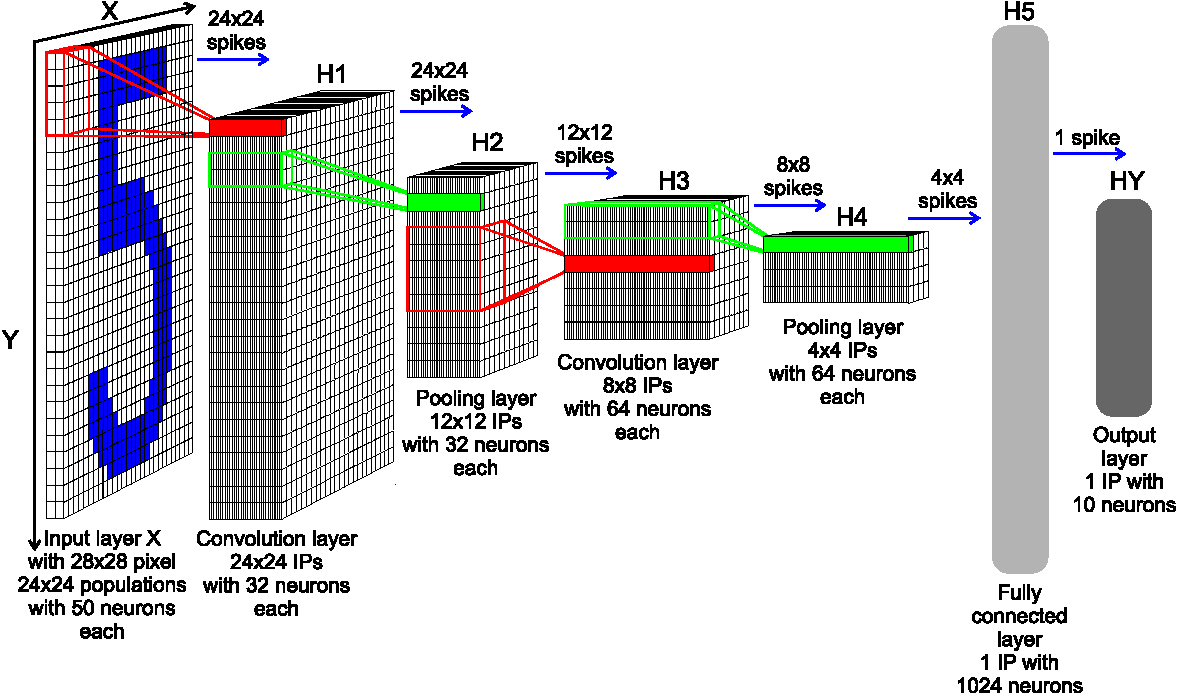
\includegraphics[width=0.5\columnwidth]{./chapters/sbs_accelerator/figures/sbs_network.pdf}
	\caption{\gls{sbs} network architecture for handwritten digit classification task.}
	\label{fig:sbs_network}
\end{figure*}


\begin{table}\centering
	\caption{\gls{sbs} network architecture for handwritten digit classification task.}
	\label{tab:sbs_network}
	\scriptsize
	\begin{tabular}{lrrrrrrr}\toprule
		&\multicolumn{3}{c}{\textbf{Layer size}} & &\multicolumn{2}{c}{\textbf{Kernel size}} \\\cmidrule{2-4}\cmidrule{6-7}
		\textbf{Layer} ($H^l$) &$N_X$ &$N_Y$ &$N_H$ & &$K_X$ &$K_Y$ \\\midrule
		Input ($HX$) &28 &28 &2 & &- &- \\
		Convolution ($H1$) &24 &24 &32 & &5 &5 \\
		Pooling ($H2$) &12 &12 &32 & &2 &2 \\
		Convolution ($H3$) &8 &8 &64 & &5 &5 \\
		Pooling ($H4$) &4 &4 &64 & &2 &2 \\
		Fully connected ($H5$) &1 &1 &1024 & &4 &4 \\
		Output ($HY$) &1 &1 &10 & &1 &1 \\
		\bottomrule
	\end{tabular}
\end{table}

\paragraph{Computational Cost}

The number of \gls{mac} operations required for inference of an \gls{sbs} layer is defined by $NOPS_{MAC}=N_{Spk} N_X N_Y K_X K_Y (3 N_H + 2)$, where $N_{Spk}$ is the number of spikes (iterations), $N_X N_Y$ is the size of the layer, $K_X K_Y$ is the size of the kernel for convolution/pooling, and $N_H$ is the length of $\vec{h}$. The computational cost of \gls{sbs} network models is higher compared to equivalent \gls{cnn} models and lower compared to regular \gls{snn} models (e.g., \gls{lif}) \mbox{\cite{izhikevich2004model}}.


\begin{figure*}
	\centering
	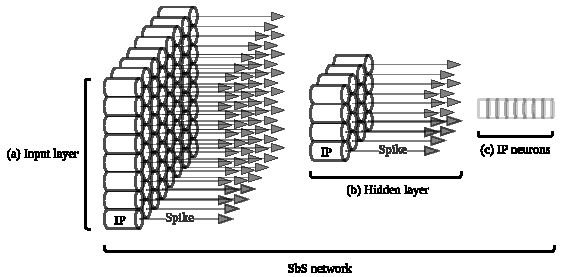
\includegraphics[width=0.5\columnwidth]{./chapters/sbs_accelerator/figures/SbS_layer.pdf}
	\caption{\gls{sbs} \glspl{ip_sbs} as independent computational entities, (a) illustrates an input layer with a massive amount of \glspl{ip_sbs} operating as independent computational entities, (b) shows a hidden layer with an arbitrary amount of \glspl{ip_sbs} as independent computational entities, (c) exhibits a set of neurons grouped in an \gls{ip_sbs}.}
	\label{fig:SbS_layer}
\end{figure*}


\paragraph{Error Tolerance}

To illustrate the error tolerance of \gls{sbs} networks, it is presented a classification performance under positive additive uniformly distributed noise as external disturbance. \fig{fig:robustnes_sbs} presents a comparison of the classification performance of an \gls{sbs} network and a standard \gls{cnn}, with the same amount of
neurons per layer as well as the same layer structure. Both neural networks are trained for handwritten digit classification on MNIST dataset \cite{lecun1998mnist} (see \cite{rotermund2019Backpropagation} for details). The figure shows the correctness for the MNIST test set with its \num[group-separator={,}]{10000} patterns in dependency of the noise level for positive additive
uniformly distributed noise. The blue curve shows the performance for
the \gls{cnn}, while the red curve shows the performance for
the \gls{sbs} network with \num[group-separator={,}]{1200} spikes (iterations). Beginning
with a noise level of 0.1, the respective performances are different
with a p - level of at least $10^{-6}$ (tested with the Fisher exact
test). Increasing the number of spikes per \gls{sbs} population to \num[group-separator={,}]{6000}
(performance values shown as black stars), shows that more spikes can
improve the performance under noise even more.

\begin{figure*}
	\centering
	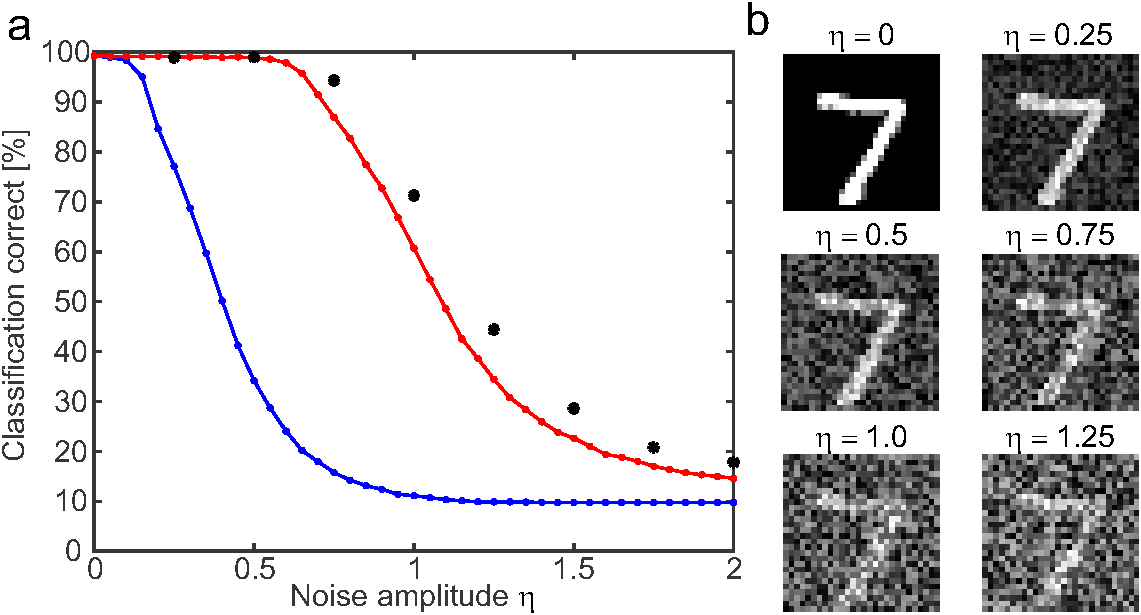
\includegraphics[width=0.5\columnwidth]{./chapters/sbs_accelerator/figures/sbs_robustnes.pdf}
	\caption{(a) Performance classification of \gls{sbs} NN versus equivalent \gls{cnn}, and (b) example of the first pattern in the MNIST test data set with different amounts of positive additive uniformly distributed noise.}
	\label{fig:robustnes_sbs}
\end{figure*}
\FloatBarrier

\section{Conventional Artificial Neural Networks}
\glspl{ann} represent the main pillar in the \gls{ai}/\gls{ml} domain. Drawing inspiration from the networks of neurons in the human brain, \glspl{ann} have been designed to process information through interconnected nodes or "neurons". The concept of neural networks traces its roots back to the 1950s with the introduction of the perceptron by Frank Rosenblatt. The perceptron, a single-layer feedforward neural network, was among the first models capable of binary classifications~\cite{rosenblatt1958perceptron}. However, the limitations of perceptrons, including their inability to solve non-linearly separable functions, led to diminished interest in neural networks until the backpropagation algorithm emerged in the 1980s~\cite{rumelhart1986learning}. \glspl{ann} are designed to learn from data, allowing them to perform tasks without being explicitly programmed. Following this introduction, this section explores \glspl{ann}, with a particular focus on the specifics of \glspl{cnn}.

\subsection{Architecture}

Neural networks are computational models designed to extract patterns, interpret data, and approximate complex functions. Their architecture comprises interconnected nodes (neurons) organized into layers. Each connection possesses a weight value, which is adjusted during training. The primary components include:

\subsubsection{Layers}

\begin{itemize}
	\item \textbf{Input Layer}: Receives data. Given input data vector \( \mathbf{x} \) of dimension \( d \), the number of neurons is \( d \).
	\[
	\mathbf{x} = [x_1, x_2, ..., x_d]^\intercal
	\]
	
	\item \textbf{Hidden Layer(s)}: Transform the input using weighted connections. The output \( h \) of a neuron in a hidden layer is:
	\[
	h = f(\mathbf{w^\intercal} \cdot \mathbf{x} + b)
	\]
	where \( \mathbf{w} \) is the weights vector, \( b \) is a bias, and \( f \) is an activation function.
	
	\item \textbf{Output Layer}: Produces the predictions. The architecture depends on the task (e.g., regression, classification).
\end{itemize}

\subsubsection{Weights and Bias}

For each neuron, input data is transformed using weights and biases, adjusted during training. The weighted sum for neurons is defined as:
\[
z = \mathbf{w^\intercal} \cdot \mathbf{x} + b
\]

\subsubsection{Activation Functions}

The activation functions introduce non-linearities, enabling neural networks to capture complex relationships. Common functions include:

\begin{itemize}
	\item \textbf{Sigmoid}: 
The sigmoid function, denoted as \( \sigma(z) \), is especially used in binary decision tasks. Mathematically, the sigmoid function is defined as:

\[
\sigma(z) = \frac{1}{1 + e^{-z}}
\]

Here, \( z \) represents the input to the function. The function outputs a value between 0 and 1, making it especially useful for models where the output is a probability. 

The curve of the sigmoid function is S-shaped or sigmoidal. One of its properties is that its derivative (used in the backpropagation step of training neural networks) can be expressed in terms of the sigmoid function itself:

\[
\sigma'(z) = \sigma(z)(1 - \sigma(z))
\]

However, the sigmoid function is not without drawbacks. For very large or very small values of \( z \), the function becomes saturated, leading to small gradients and, consequently, slow convergence during training~\cite{glorot2010understanding}. This phenomenon is often referred to as the "vanishing gradient" problem.
	
	\item \textbf{Tanh}: 
The hyperbolic tangent function, denoted as \( \tanh(z) \), serves as an activation function in many neural network architectures. It scales and shifts the output of the sigmoid function to produce outputs in the range \([-1, 1]\). The mathematical expression for \( \tanh \) is:

\[
\tanh(z) = \frac{e^{z} - e^{-z}}{e^{z} + e^{-z}}
\]

Alternatively, it can be expressed in terms of the sigmoid function, \( \sigma(z) \), as:

\[
\tanh(z) = 2\sigma(2z) - 1
\]

The derivative of \( \tanh \), which is used during the backpropagation phase of neural network training, is given by:

\[
\frac{d}{dz}\tanh(z) = 1 - \tanh^2(z)
\]

Compared to the sigmoid function, \( \tanh \) is often preferred because its outputs are zero-centered, making it less likely to get stuck during training. However, it still suffers from the vanishing gradient problem for very large or very small values of \( z \).
	
	\item \textbf{ReLU}: 
The Rectified Linear Unit, commonly referred to as ReLU, has become one of the default activation functions, particularly for deep learning architectures. Mathematically, the ReLU function is defined as:

\[
f(z) = \max(0, z)
\]

In essence, the function returns \( z \) if \( z \) is greater than or equal to zero, and returns zero otherwise. This can be visualized as a linear function that will output the input directly if it is positive; otherwise, it will output zero.

The gradient of the ReLU function is binary:

\[
f'(z) = 
\begin{cases} 
1 & \text{if } z > 0 \\
0 & \text{otherwise}
\end{cases}
\]

One noted benefit of the ReLU function is its computational efficiency, given that it only requires a simple thresholding at zero. This allows models to train faster and requires less computational resources compared to other activation functions like sigmoid or tanh.

However, a potential drawback of the ReLU function is that units can sometimes get "stuck" during training and cease updating, leading to what's known as "dying ReLUs." The dying ReLU phenomenon can be viewed as a specific type of the vanishing gradient problem, where ReLU neurons become non-responsive and consistently output a value of zero, regardless of the input they receive. This is due to the fact that for inputs less than 0, the gradient is 0, which can cause weights to not update during backpropagation. To counteract this, variants like Leaky ReLU~\cite{maas2013rectifier} and Parametric ReLU~\cite{he2015delving} have been proposed.
\item \textbf{Softmax}:
In a neural network for multiclass classification tasks, the softmax function is a common choice for the activation function in the output layer. Given an input vector \( \mathbf{z} \) of length \( K \), representing the raw output (logits) of the \( K \) nodes in the output layer, the softmax function transforms these logits into a probability distribution over \( K \) classes. For each component \( i \) (where \( i = 1, 2, \ldots, K \)), the softmax function \( S(\mathbf{z}) \) is computed as:
\[
S(\mathbf{z})_i = \frac{{\exp(z_i)}}{{\sum_{j=1}^{K} \exp(z_j)}}
\]
where \( S(\mathbf{z})_i \) represents the \( i \)-th component of the output vector \( S(\mathbf{z}) \), \( \exp \) denotes the exponential function, and \( z_i \) is the \( i \)-th component of the input vector \( \mathbf{z} \). After applying the softmax function, each component of \( S(\mathbf{z}) \) is in the interval \( (0, 1) \), and the components sum to 1, allowing them to be interpreted as probabilities associated with each of the \( K \) classes. This makes the softmax function particularly useful for producing the final output in a neural network designed for classification tasks, as it ensures that the outputs are normalized and can be interpreted as class probabilities.

\end{itemize}

\subsection{Training Process}

Neural networks learn by adjusting weights and biases in response to training data. The goal is to minimize the difference between predictions and target values (the loss), often optimized using gradient-based methods.

\subsubsection{Stochastic Gradient Descent}

\gls{sgd} is an iterative optimization algorithm used to minimize an objective function that is defined as a sum of differentiable functions. This is particularly well-suited for problems with a large number of training samples~\cite{bottou2010large}.

Given an objective function \( J(\theta) \) which we aim to minimize, the objective is often defined as:
\[
J(\theta) = \frac{1}{N} \sum_{i=1}^{N} J_i(\theta)
\]
where \( J_i(\theta) \) is the loss associated with the \( i^{th} \) training example and \( \theta \) represents the parameters of the model.

The basic update rule for \gls{sgd} is:
\[
\theta \leftarrow \theta - \eta \nabla J_i(\theta)
\]
where:
\begin{itemize}
	\item \( \eta \) is the learning rate, a positive scalar determining the size of steps in the parameter space.
	\item \( \nabla J_i(\theta) \) is the gradient of the loss with respect to the parameters for the \( i^{th} \) training example.
\end{itemize}

In each iteration, a single training example \( (x_i, y_i) \) is picked randomly, and the model parameters are updated with the gradient of the loss \( J_i(\theta) \) with respect to that single example.

The iterative nature and use of only a single training example at each step make \gls{sgd} computationally more efficient compared to batch gradient descent, especially for large datasets~\cite{bottou2010large}. However, due to its stochastic nature, the trajectory of the parameters through the parameter space can be noisy, leading to a non-stable convergence to the minimum~\cite{bottou2018optimization}. Variants and improvements, like momentum~\cite{sutskever2013importance} or adaptive learning rates~\cite{duchi2011adaptive}, have been introduced to combat this instability and accelerate convergence.

\subsection{Multi-Layer Perceptron}

A \gls{mlp} is a type of feedforward artificial neural network, consisting of multiple layers of interconnected neurons~\cite{goodfellow2016deep}.

\subsubsection{Key Components}

\begin{itemize}
	\item An \textbf{input layer} that receives the data. The number of neurons in this layer corresponds to the dimensionality of the input data.
	
	\item One or more \textbf{hidden layers} that transform the input data. Each neuron in a hidden layer computes a weighted sum of its inputs, adds a bias term, and then applies an activation function.
	
	\item An \textbf{output layer} that provides the final prediction or classification results. The number of neurons in the output layer and their activation functions are tailored to the specific task.
\end{itemize}

Mathematically, the output \( o_{j} \) of the \( j^{th} \) neuron in any layer can be defined as:

\[
o_{j} = f\left( \sum_{i=1}^{N} w_{ij} x_{i} + b_{j} \right)
\]

where:
\begin{itemize}
	\item \( x_{i} \) is the output of the \( i^{th} \) neuron from the previous layer.
	\item \( w_{ij} \) is the weight associated with the connection between the \( i^{th} \) neuron from the previous layer and the \( j^{th} \) neuron of the current layer.
	\item \( b_{j} \) is the bias term for the \( j^{th} \) neuron.
	\item \( f \) is the activation function, which introduces non-linearity into the network.
\end{itemize}

The weights and biases of an \gls{mlp} are adjusted during the training phase.


\subsection{Convolutional Neural Networks}

\glspl{cnn} represent a specialized architecture in the deep learning domain, predominantly optimized for image and video processing tasks. Drawing inspiration from the human visual cortex structure and function, \glspl{cnn} are adept at automatically and adaptively discerning spatial hierarchies and patterns inherent in visual data~\cite{lecun1998gradient}.

\subsubsection{Key Components}

\begin{itemize}
	\item \textbf{Input Layer}: Responsible for ingesting raw pixel values from the image. The size is typically dictated by the resolution and depth (e.g., RGB channels) of the input.
	
	\item \textbf{Convolutional Layer}: At its core, the convolution operation involves sliding a filter over the input matrix to produce feature maps. Each filter aims to detect specific features, like edges or textures, in the input. Mathematically, a convolutional layer applies a set of learnable filters (or kernels) to the input data, where each filter is convolved across the width and height of the input volume, computing the dot product between the entries of the filter and the input, resulting in a two-dimensional activation map. This operation captures local dependencies in the input through spatial relationships.
	
	\item \textbf{Activation Function}: Following the convolution operation, it is common to introduce non-linearity into the system. The ReLU is popularly employed in \glspl{cnn}.
	
	\item \textbf{Pooling Layer}: To reduce the spatial dimensions and computational load, the pooling layer down-samples feature maps. Max pooling is a widely adopted strategy. Given an input matrix \(X\) with dimensions \(W \times H\), max pooling operates over non-overlapping subregions defined by a \(n \times m\) window and stride \(S\). Each element \(Y_{ij}\) in the output matrix \(Y\) is computed as \(Y_{ij} = \max \{X_{kl}\}\), where the maximum is taken over the elements \(X_{kl}\) from the pooling window. This procedure reduces the dimensions of the output to \(\left\lceil \frac{W - n}{S} + 1 \right\rceil \times \left\lceil \frac{H - m}{S} + 1 \right\rceil\), assuming no padding.
	
	\item \textbf{Fully Connected Layer}: This layer sees each neuron connected to every activation from the previous layer, effectively acting as a standard multi-layer perceptron. It linearizes the features extracted from preceding layers and approximates a function, which commonly is an image classification or regression task.
	
	\item \textbf{Output Layer}: For classification tasks, a common approach is to employ a fully connected layer with a softmax activation function, transforming the output into probability distributions across the classes, in binary classification scenarios a single neuron with sigmoid activation is commonly utilized. For regression tasks, to predict continuous values, it is typically used an output layer with a single neuron (or multiple neurons corresponding to the dimensionality of the output) without an activation function or with a linear one. 
\end{itemize}

A relevant characteristic of \glspl{cnn} is weight sharing, this substantially reduces the number of parameters, thus diminishing the risk of overfitting. Through their capacity to hierarchically discern two-dimensional patterns, \glspl{cnn} have been relevant in furthering advancements in a variety of fields, spanning from sensor analytics to medical image analysis and autonomous vehicle vision systems.

\subsubsection{Conv2D Tensor Operation}
A convolutional layer aims to learn and extract feature representations from a given input. Each unit of a feature map is connected to a region of neighboring units on the input maps (from the previous layer). This neighborhood in the previous layer is known as the receptive field of such unit. A new feature map can be obtained by first convolving the input maps with a learned kernel and then applying a nonlinear elementwise activation function to the convolved results. All spatial locations on the input maps share a kernel to generate a feature map. All feature maps are obtained by convolving several different kernels~\cite{gu2018recent}.


The 2D convolution process is performed by the \emph{Conv2D} tensor operation, described in \Equ{eq:conv2D}, where $W$ is the convolution kernels (known as filters), $b$ is the bias vector for the output feature maps, and $h$ is the input tensor containing the feature maps~\cite{goodfellow2016deep}. $K\times L\times M$ is the receptive field size, $K\times L$ is the convolution kernel, and $M$ is the number of input channels/feature maps. Mathematically, the \emph{Conv2D} operator is defined as:
\begin{eqnarray} \label{eq:conv2D}
Conv2D\left(W,b,h\right)_{i,j,o}=\sum_{k,l,m}^{K,L,M} h_{(i+k,j+l,m)} W_{(o,k,l,m)}+b_{o}
\end{eqnarray}

\subsubsection{Computational Cost of a Convolution Layer}

The computational cost of a convolution layer primarily depends on the spatial dimensions of the input and the kernel, the number of input and output channels, and the stride (slide step) with which the kernel is applied. A list of definitions and concepts is presented:

\paragraph{Definitions}
\begin{itemize}
	\item \( W_i \): Width of the input feature map.
	\item \( H_i \): Height of the input feature map.
	\item \( D_i \): Depth (number of channels) of the input feature map.
	\item \( W_k \): Width of the kernel.
	\item \( H_k \): Height of the kernel.
	\item \( D_k \): Depth of the kernel. Typically, \( D_k = D_i \).
	\item \( N_o \): Number of output feature maps (number of kernels in the layer).
	\item \( S \): Stride of the convolution.
\end{itemize}

\paragraph{Computations Per Output Element}

For each kernel position on the input feature map, the number of multiply and accumulate operations is defined by:
\begin{equation}
2 \times W_k \times H_k \times D_k
\end{equation}

\paragraph{Output Dimensions}

Given the stride \( S \), the dimensions of the output feature map are:
\begin{align}
W_o &= \frac{W_i - W_k}{S} + 1 \\
H_o &= \frac{H_i - H_k}{S} + 1
\end{align}

\paragraph{Total Computations}

For each output feature map, the total operations are:
\begin{equation}
W_o \times H_o \times 2 \times W_k \times H_k \times D_k
\end{equation}

Given \( N_o \) output feature maps, the computational cost of an entire convolution layer becomes:
\begin{equation}
N_o \times W_o \times H_o \times 2 \times W_k \times H_k \times D_k
\end{equation}

This represents the number of multiply-accumulate operations in a convolution layer. Other considerations might include biases and employed activation functions, but the above calculation primarily signifies the computational burden of the convolution operation.

\subsubsection{Error Tolerance in Convolution Layers}

Deep neural networks, especially \glspl{cnn}, have exhibited an advantageous property: they possess a significant degree of robustness to various perturbations in their computations, including reduced-precision arithmetic and the introduction of noise. This error tolerance has been exploited for various optimization techniques with the goal of reducing computational and storage overhead without sacrificing too much performance~\cite{han2015deep}.

\paragraph{Sources of Error}

Errors in convolution layers can arise from various sources:
\begin{itemize}
	\item \textbf{Quantization:} Converting \gls{fp} precision weights and activations to a lower bit-width representation.
	\item \textbf{Pruning:} Setting certain weights to zero to reduce the total number of weights.
	\item \textbf{Approximate Computing:} Techniques that purposefully introduce computational errors by simplifying compute hardware to improve power efficiency, area, and speed.
\end{itemize}

\paragraph{Error Compensating Mechanisms}

There are several hypotheses and mechanisms that explain the error tolerance:

\begin{itemize}
	\item \textbf{Overparameterization:} Many deep models have more parameters than necessary for the task. This data redundancy can help the network adapt to small errors.
	\item \textbf{Re-training:} After introducing errors (like in quantization), the network can be fine-tuned to recover some of the lost performance.
	\item \textbf{Regularization Effect:} Some error introduction techniques, like quantization, can act as a form of regularization, potentially helping to prevent overfitting.
\end{itemize}

\paragraph{Exploiting Error Tolerance for Optimization}

Leveraging the error resilience of convolution layers can lead to several benefits:

\begin{itemize}
	\item \textbf{Reduced Precision:} Weights and activations can be represented with fewer bits, leading to a reduced memory footprint and computation savings.
	\item \textbf{Energy Efficiency:} Approximate computing techniques can yield significant power savings.
	\item \textbf{Faster Computations:} Reduced precision arithmetic can be faster, requiring reduced computational hardware requirements, and can allow higher parallelism.
\end{itemize}

Understanding and harnessing the error tolerance properties of convolution layers present opportunities for designing more efficient and compact neural network implementations, especially vital for low-power devices and real-time applications. While errors can be introduced to an extent, it remains crucial to ensure that the network accuracy does not degrade beyond acceptable levels.


\section{Neural Network Accelerators}
Neural network accelerators are specialized hardware components or platforms designed to accelerate the computationally intensive tasks associated with neural networks. Their primary goal is to enhance performance, reduce power consumption, and provide real-time processing capabilities for \gls{ai}/\gls{ml} applications~\cite{sze2017efficient}.

\subsection{The Need for Accelerators}
Neural networks come with intensive computational and memory demands due to their deep architectures and vast numbers of parameters:

\begin{itemize}
	\item \textbf{Compute Cost}: \gls{ai}/\gls{ml} models, especially \glspl{cnn} and transformers, are characterized by their deep architectures. Each layer involves a large number of weights and activations. In the forward pass (inference), for each neuron, the input activations are multiplied by corresponding weights, and then all these products are accumulated to produce the neuron output. Similarly, during training, the backpropagation algorithm is also computation-costly.
	
	\item \textbf{Memory Cost}: \gls{ai}/\gls{ml} models, especially those with millions or even billions of parameters, require elevated memory footprint for model storage. During computation, the frequent access to weights, along with the need to read and write intermediate activations, can stress the memory bandwidth. Memory access is also energy-expensive, often more than the actual arithmetic operations.
	
	As illustration, the memory requirements for an \gls{mlp} are:
	\begin{enumerate}
		\item \textbf{Weights Storage}: Given a deep neural network with \(L\) layers, where each layer \(l\) has \(n_l\) neurons and receives input from \(n_{l-1}\) neurons, the number of weights (excluding biases) is:
		\begin{align*}
		W &= \sum_{l=2}^{L} n_l \times n_{l-1}
		\end{align*}
		
		\item \textbf{Activations Storage}: Activations need to be stored for the forward pass and are particularly crucial during training for the backpropagation process. For a given layer \(l\), activations storage requirement is proportional to \(n_l\), and the total for the entire network is:
		\begin{align*}
		A &= \sum_{l=1}^{L} n_l
		\end{align*}
	\end{enumerate}
	Considering both weights and activations, the memory access pattern becomes a bottleneck, especially when the model size exceeds the on-chip memory capacity, leading to frequent off-chip accesses which are both time and energy-consuming.
	
	\item \textbf{Real-time Requirements}:
	Many contemporary applications demand instantaneous or near-instantaneous processing due to their interactive or safety-critical nature. Hence, the computational backend supporting such applications, often driven by deep neural networks, must be optimized for low-latency and high-throughput to meet the real-time requirements.
	
	\item \textbf{Energy Efficiency}: Many modern devices, from smartphones to \gls{iot} sensors, operate on constrained power budgets, such as batteries. For these devices, the power-hungry computations of \gls{ai}/\gls{ml} models can quickly drain the power sources, limiting usability, applicability, and functionality. Given that neural network computations are becoming pervasive, even in these power-constrained devices, energy efficiency is of vital importance.
	
	The proliferation of \gls{ai}/\gls{ml} applications in low-power devices imposes strict constraints on energy consumption. Factors driving this need include:
	
	\begin{enumerate}
		\item \textbf{Constrained Power Sources}: Most low-power devices rely on battery power. High energy consumption due to intensive computations can drastically reduce operational time between charges, affecting applicability.
		
		\item \textbf{Form Factor and Heat Dissipation}: Smaller devices have smaller batteries and reduced space for cooling mechanisms, making them susceptible to overheating. Hence, energy-efficient computations are not only related to battery longevity but also about device temperature, safety, and size.
		
		\item \textbf{Operational Continuity in Low-Power Devices}: Many edge devices, such as sensors, are expected to operate continuously. These devices might be located in hard-to-reach places, making frequent battery replacements impractical. Thus, energy efficiency is crucial for operational viability and application feasibility.
	\end{enumerate}
	
\end{itemize}

Given these challenges, it is needed to optimize neural network deployments on such devices at both software and hardware levels to achieve desired performance within the power constraints.

\subsection{Types of Accelerators}

In the dynamic field of \gls{ai}/\gls{ml}, various hardware accelerators, including \glspl{gpu}, \glspl{asic}, \glspl{fpga}, and \glspl{npu}, have emerged to optimize and facilitate neural network computations.
\begin{itemize}
	\item \textbf{\glspl{gpu}}: Historically designed for the purpose of graphics rendering, \glspl{gpu} have architecture that naturally perform parallel computing. This parallelism is especially beneficial for neural network computations involving repetitive and simultaneous operations. As a result, \glspl{gpu} have become essential for deep learning training and inference.
	
	The success of \glspl{gpu} in the \gls{ai}/\gls{ml} domain is evident from the rise of \gls{gpu}-optimized deep learning frameworks and the continuous evolution of \gls{gpu} architectures tailored for neural network computations.
	
	
	\item \textbf{\glspl{asic}}: These can provide significant benefits in terms of power, performance, and area over general-purpose processors. One of the most notable \glspl{asic} designed for neural network computations is Google's \gls{tpu}. Neuromorphic chips, like IBM's TrueNorth or Intel's Loihi, are \glspl{asic} designed to mimic the synapse-neuron connections in the human brain, potentially offering more efficient ways to handle neural network tasks, especially for real-time processing and low-power scenarios.
	
	\item \textbf{\glspl{fpga}}: \glspl{fpga} represent a bridge between general-purpose processors and \glspl{asic} in terms of adaptability and performance:
	
	\begin{enumerate}
		\item \textbf{Reconfigurability}: Unlike \glspl{asic}, which are fixed in their functionality post-manufacture, \glspl{fpga} can be reconfigured to adopt different logic functions. This means they can be tailored to accelerate specific neural network operations or configured to perform certain computational patterns.
		
		\item \textbf{Parallelism}: \glspl{fpga} excel in parallel processing, with their array of logic blocks and interconnects. Neural network computations, which often involve concurrent operations on data, can be accelerated by exploiting this parallelism.
		
		\item \textbf{Prototyping and Evolution}: Given their reconfigurable nature, \glspl{fpga} are excellent platforms for prototyping neural network architectures. Furthermore, in environments where neural network models evolve or are frequently updated, \glspl{fpga} can adapt without requiring new hardware, even during an ongoing operation.
		
		\item \textbf{Trade-offs}: While \glspl{fpga} offer flexibility, they might not achieve the same level of performance or energy efficiency as a highly-optimized \gls{asic} for a specific task. However, their adaptability can outweigh this in certain scenarios.
	\end{enumerate}
	
	In the context of the rapidly evolving field of \gls{ai}/\gls{ml}, \glspl{fpga} provide a compelling balance of adaptability and performance, especially when agility in hardware is desired.
	
	\item \textbf{\glspl{npu}}: These are dedicated hardware accelerators optimized for neural network computation. \glspl{npu} streamline both training and inference processes by focusing on operations and data flow patterns typically found in neural networks, resulting in enhanced energy efficiency and performance compared to general-purpose processors.
	
\end{itemize}

\subsection{Design Considerations}
For neural network accelerator design, it is important to address key considerations such as precision, memory hierarchy, scalability, and flexibility, each of which plays a crucial role in ensuring optimal performance and adaptability in the evolving \gls{ai}/\gls{ml} domain.

\begin{itemize}
	\item \textbf{Precision}: In neural network accelerator design, the precision of arithmetic operations plays an important role. Employing reduced precision arithmetic offers dual advantages: it can markedly accelerate computations and simultaneously diminish power consumption. However, it is crucial to preserve a balance to ensure that the reduced precision does not compromise the accuracy and reliability of the neural network model.
	
	\item \textbf{Memory Hierarchy and Dataflow}: Memory hierarchy and dataflow are tightly coupled in the design of efficient neural network accelerators. Dataflow refers to the way data is passed and processed between different memory hierarchies and computation units. The choice of dataflow can dramatically impact the energy efficiency, latency, and throughput of the accelerator.
	
	For neural networks, especially deep learning models, the memory access pattern plays a significant role in determining overall performance. This is because fetching data (e.g., weights, activations) from memory often consumes more energy and time than the arithmetic computations themselves.
	\item \textbf{Scalability}: The capability of a neural network accelerator to extend its computational capacity to handle larger neural networks or to elevate existing hardware performance. This extension can be achieved by either increasing the resources within a single chip (vertical scaling) or by distributing the computation across multiple chips or processing units (horizontal scaling).
	
	As neural network models become more complex and demand more computational resources, it is crucial for accelerators to be scalable. This ensures that they can continue to provide accelerated performance for newer and larger models without requiring a complete redesign.
	A modular approach facilitates easy addition of processing units or modules to address scalability needs.
	\item \textbf{Flexibility}: Flexibility remains a cornerstone in the design of neural network accelerators. While tailoring hardware for specific tasks or models can yield substantial performance boosts, it is imperative that these accelerators retain the versatility to accommodate a diverse range of neural network models and operations. This ensures a balance between optimized performance and broad applicability, allowing for both efficiency and adaptability in an ever-evolving field.
	
\end{itemize}

\section{Precision and Effect in Training}

Conventional neural networks typically rely on standard \gls{fp} arithmetic. However, to elevate computational speed, minimize memory footprint, and reduce energy consumption, hardware accelerators adopt lower precision formats. While this can speed up operations and reduce resource demands, there is a trade-off as reduced precision might affect the model accuracy. Therefore, balancing precision and performance is crucial, with techniques such as mixed-precision and dynamic/custom arithmetic being employed to navigate these trade-offs~\cite{micikevicius2017mixed}.
\subsection{Fixed-Point}

Fixed-point arithmetic represents numbers with a fixed number of digits before and after the decimal point, in contrast to floating-point where the decimal point can "float". Leveraging fixed-point arithmetic offers distinct advantages. Specifically, fixed-point operations are more resource-efficient, leading to accelerated computations. Additionally, their inherent simplicity in arithmetic operations often translates to diminished power consumption. 


However, while fixed-point arithmetic offers efficiencies in many neural network applications, there are situations where it may not be ideal:

\begin{enumerate}
	\item \textbf{Training}: During training, the need to represent small weight updates and gradient values is critical. \gls{fp} arithmetic is often preferred to ensure effective backpropagation, whereas fixed-point might impede convergence or acceptable model accuracy~\cite{courbariaux2014training}.
	
	\item \textbf{High-Precision}: For precision-critical tasks, such as medical, fixed-point arithmetic might compromise prediction accuracy, especially when using fewer bits.
	
	\item \textbf{Transfer Learning and Fine-Tuning}: In scenarios such as fine-tuning pre-trained models, small gradient values are crucial. The reduced precision of fixed-point might neglect these refined updates.
	
	\item \textbf{Normalizing and Batch Normalization}: Operations involving a diverse range of values, like normalization, might introduce significant quantization errors when using fixed-point representations~\cite{jacob2018quantization}.
	
	\item \textbf{\glspl{rnn}}: Due to their sequential nature and sensitivity to numerical precision, these models are particularly prone to amplified errors from precision loss during the sequential processing of data. This issue is especially prominent in tasks involving long sequences or those requiring high precision.
	
	\item \textbf{Activation Functions with Exponential Ranges}: Functions such as softmax, which operate over a wide range, might be susceptible to quantization errors in a fixed-point context.
\end{enumerate}

While quantization techniques continue to evolve, it remains essential to rigorously evaluate fixed-point representations in the above contexts to ensure desired performance and accuracy.



\subsection{Floating-Point}
\gls{fp} arithmetic offers distinct advantages due to its capability to represent numbers with both high precision and a wide dynamic range. However, while it provides granular accuracy, it typically demands more computational resources and power compared to fixed-point arithmetic. The inherent robustness of neural networks to numerical perturbations implies a potential avenue for exploring custom reduced-precision \gls{fp} arithmetic.

The representation of every numerical value, in any numerical system, is made of an integer and a fractional part. The border that delimits them is called the radix point. The fixed-point format for representing numeric values derives its name from the fact that in this format, the base point is fixed at a certain position. For integer numbers, this position is at the right of the least significant digit.

In scientific computation, it is often necessary to represent very large and very small values. This is difficult to achieve using the fixed-point format because the bit size required to maintain both the desired precision and the desired range are very large. In such situations, \gls{fp} formats are used to represent real numbers. Each \gls{fp} number can be divided into three fields: sign $S$, exponent $E$, and mantissa $M$. Using the binary number system, it is possible to represent any \gls{fp} number as:

\begin{eqnarray} \label{eq:float}
(-1)^{S} \times 1.M \times 2^{E-B}
\end{eqnarray}

In \gls{fp} representations the exponent is biased. This bias depends on the bit size of the exponent field. This exponent bias is defined by \Equ{eq:float_bias}, where $E_{size}$ is the exponent bit size.

\begin{eqnarray} \label{eq:float_bias}
B=2^{E_{size}-1}-1
\end{eqnarray}

There is a natural trade-off between small bit size requiring fewer hardware resources and larger bit size providing higher precision. Within a given total bit size, it is possible to assign various combinations of sizes to the exponent and mantissa fields, with wider exponents resulting in a higher range and wider mantissa resulting in better precision.

The most widely used format for \gls{fp} arithmetic is the IEEE 754 standard \cite{zuras2008ieee}. The IEEE single-precision format (32-bit) is expressed by \Equ{eq:float} with $B$ = 127, 8 bits for the exponent and 23 bits for the mantissa, see \Fig{fig:floating}(a). In \gls{fp} formats, the numbers are normalized, the leading one is an implicit bit, and only the fractional part is explicitly stored in the mantissa field.

\begin{figure*}
	\centering
	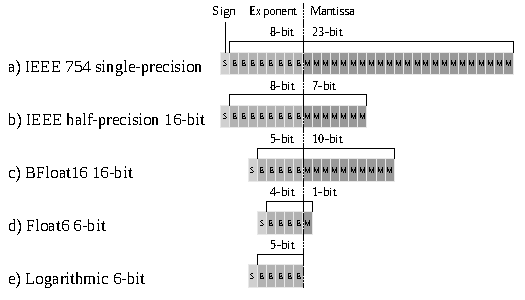
\includegraphics[width=0.5\columnwidth]{./chapters/cnn_accelerator/figures/power_breakdown/floating_point.pdf}
	\caption{Floating-point number representation.}
	\label{fig:floating}
\end{figure*}

Reduced bit size than those specified in the IEEE 754 standard are often sufficient to provide the desired precision. Reduced designs require fewer hardware resources enabling low-power implementations. In custom hardware designs, it is possible to customize the \gls{fp} format implemented. In later sections, the term E$a$M$b$ is used to denote \gls{fp} formats, where $a$ and $b$ are the exponent and mantissa bit size, respectively. For example, E4M1 means 4-bit exponent and 1-bit mantissa, see \Fig{fig:floating}(d).

There are three special definitions in IEEE 754 standard. The first is subnormal numbers when $E=0$, then \Equ{eq:float} is modified to \Equ{eq:float_subnorm}. Infinity and \gls{nan} are the other two special cases but are not used in this research. Infinite and \gls{nan} values often indicate undefined operations or errors in calculations (such as division by zero, logarithm of a negative number, etc.). These values do not represent meaningful information that can be used for learning patterns from data. Consequently, this can lead to simplified hardware complexity in custom \gls{fp} neural network accelerators by streamlining the control logic.

\begin{eqnarray} \label{eq:float_subnorm}
(-1)^{S} \times 0.M \times 2^{1-B}
\end{eqnarray}

\subsection{Post-Training Quantization}
Transitioning a neural network model from high-precision to lower-precision computations presents a set of challenges. One of the most critical of these challenges lies in preserving the accuracy of the model while it operates under conditions of reduced numerical precision. This balance requires thoughtful consideration and strategic implementation to ensure that the benefits of computational efficiency do not come at the cost of significant degradation in model performance.

In \gls{ptq}, a neural network, once fully trained, undergoes a conversion process wherein its \gls{fp} weights and activations are mapped to a lower precision~\cite{krishnamoorthi2018quantizing}.

Given the full precision weights \( W \) of a neural network, they can be quantized to a lower precision using the quantization function:
\begin{equation}
Q(W) = \text{round}\left(\frac{W}{\Delta}\right) \times \Delta
\end{equation}
where \( \Delta \) is a quantization step size, often derived from the range of the weights or activations and the target precision.

One challenge of \gls{ptq} is to ensure minimal loss of accuracy after the conversion. Techniques such as fine-tuning the quantized model, applying regularization during initial training, or using advanced quantization schemes (e.g., mixed precision) can help to preserve the model accuracy.

While \gls{ptq} offers the benefit of simplicity, the resultant quantized model might not be as robust or accurate as models trained with \gls{qat} techniques. However, for many applications, especially those on resource-constrained devices, the slight trade-off in accuracy is often outweighed by the benefits in computational efficiency, memory usage, and power consumption.


\subsection{Quantization-Aware Training}

This quantization maps weights to a lower precision \( Q(W) \), similarly as in \gls{ptq}; moreover, \gls{qat} integrates this process into the training phase, ensuring that the resultant model is resilient to potential accuracy degradation~\cite{krishnamoorthi2018quantizing}. Such adaptations are relevant when targeting resource-constrained devices or specialized hardware accelerators that rely on reduced precision for improved computational efficiency and accuracy.

For neural networks with custom reduced \gls{fp} formats, \gls{qat} exhibits even greater versatility. Such custom formats, often denoted as \( FP_{M,E} \), allocate specific bit-lengths for the mantissa \( M \) and the exponent \( E \). The function for this quantization format is detailed in \Algo{alg:quantizr}. This algorithm converts full-precision values into their corresponding quantized \gls{fp} representation using custom-defined exponent and mantissa bit lengths.

\begin{algorithm}[h!]
	\caption{Custom floating-point quantizer.}
	\label{alg:quantizr}
	\begin{algorithmic}
		\SetAlgoLined
		\renewcommand{\algorithmicrequire}{\textbf{input:}}
		\renewcommand{\algorithmicensure}{\textbf{output:}}
		\REQUIRE $X_{FP}$ as the \gls{fp} value.
		\REQUIRE $E_{size}$ as the target exponent bit size.
		\REQUIRE $M_{size}$ as the target mantissa bits size.
		\REQUIRE $STDM_{size}$ as the IEEE 754 mantissa bit size.
		\ENSURE $X_{CFP}$ as the custom \gls{fp} value.
		
		\STATE $sign \gets GetSign(X_{FP})$
		\STATE $exp \gets GetExponent(X_{FP})$
		\STATE $fullexp \gets 2^{E_{size}-1}-1$ // Get full range value
		\STATE $cman \gets GetCustomMantissa(X_{FP}, M_{size})$
		\STATE $leftman \gets GetLeftoverMantissa(X_{FP}, M_{size})$
		\IF {$exp <-fullexp$}
		\STATE$X_{CFP}\gets0$
		\ELSIF{$exp > fullexp$}
		\STATE$X_{CFP}\gets (-1)^{sign}\cdot2^{fullexp}\cdot(1+(1-2^{-M{size}}))$
		\ELSE
		\IF {$2^{STDM_{size}-M_{size}-1}-1<leftman$}
		\STATE $cman \gets cman+1$ // Above halfway
		\IF{$2^{M_{size}}-1<cman$}
		\STATE $cman \gets 0$ // Correct mantissa overflow
		\STATE $exp \gets exp + 1$
		\ENDIF
		\ENDIF
		\STATE // Build custom \gls{fp} representation
		\STATE$X_{CFP}\gets (-1)^{sign}\cdot2^{exp}\cdot(1+cman\cdot2^{-M_{size}})$
		\ENDIF
	\end{algorithmic}
\end{algorithm}

During training, each forward pass applies the aforementioned quantization, simulating the operational conditions of the reduced precision. The backward pass, essential for gradient-based optimization, is conducted with a higher precision. If \( \nabla W \) symbolizes the computed gradients, the weight update rule in gradient descent is typically:
\begin{equation}
W_{t+1} = W_t - \eta \nabla W
\end{equation}
Here, \( \eta \) represents the learning rate. However, with \gls{qat}, the model remains cognizant of \( Q(W) \) or \( Q_{FP}(W) \) during forward computations, a factor that influences gradient dynamics. Post-\gls{qat} calibration using a validation dataset helps to refine scaling factors or biases, this improves the model for optimal performance in its intended deployment environment. Assessments against a full-precision baseline are important to ensure that the trade-offs in precision do not compromise the model accuracy.

\section{Dataflow Taxonomy}
Dataflow taxonomy refers to the classification of various schemes that determine how data (weights, activations, and partial results) moves through the accelerator during computation. The way data is moved and reused can have an impact on the energy efficiency and throughput of the accelerator. These strategies aim to maximize performance and energy efficiency by optimizing data movement, which is often more energy-intensive than computation itself. When choosing or designing a dataflow, it is essential to consider the specific neural network workload, the memory hierarchy, and the architectural details of the hardware to ensure an optimal match~\cite{sze2017efficient}.

\subsection*{Weight Stationary (WS)}
In this dataflow, weights are kept stationary in the processing elements. As different input activations come in, they are multiplied with these stationary weights. This approach maximizes the reuse of weights, which can be beneficial when processing a large number of activations, such as during a convolution operation.
Characteristics:
\begin{align*}
\textbf{Fixed:} & \quad \text{Weights} \\
\textbf{Moving:} & \quad \text{Activations, Partial Sums}
\end{align*}

\subsection*{Output Stationary (OS)}
Here, the partial results (output activations) are kept stationary. Weights and input activations move through the processing elements and the partial sums are accumulated in place. This scheme tries to maximize the reuse of the output from the computation, which is beneficial when a given output is the result of multiple accumulations. Characteristics:
\begin{align*}
\textbf{Fixed:} & \quad \text{Partial Sums} \\
\textbf{Moving:} & \quad \text{Weights, Activations}
\end{align*}

\subsection*{Input Stationary (IS)}
In this scheme, input activations remain stationary, while weights move through and are multiplied with these stationary activations. This can be beneficial when a single activation is used in multiple computations. Characteristics:
\begin{align*}
\textbf{Fixed:} & \quad \text{Activations} \\
\textbf{Moving:} & \quad \text{Weights, Partial Sums}
\end{align*}

\subsection*{No Local Reuse (NLR)}
As the name suggests, in this dataflow, there is minimal local data reuse. All data types (weights, activations, and partial sums) move through the processing elements. This is often not as efficient in terms of energy consumption since there is a lack of reuse; however, it is simpler in terms of control and design. Characteristic:
\begin{align*}
\textbf{Moving:} & \quad \text{Weights, Activations, Partial Sums}
\end{align*}

\subsection*{Row Stationary (RS)}
This is a specialized dataflow developed for systolic array architectures. In RS, a row of the systolic array holds the activations stationary while weights are propagated horizontally and partial sums propagate vertically.


\section{Flynn's Taxonomy}

In the quest to comprehend the various computational architectures, especially when focusing on neural network accelerators and their efficiency, it is important to grasp the foundational classification of computer architectures. Flynn's Taxonomy, introduced by Michael J. Flynn in 1966, provides a categorical breakdown of architectures based on their simultaneous instruction and data streams handling capability.

\subsection*{SISD (Single Instruction, Single Data)}

This category represents the classic sequential computer architecture, where a single instruction operates on a single data stream. Most basic \glspl{cpu} can be categorized here; modern designs often include multiple cores (making them multiprocessors).

\subsection*{SIMD (Single Instruction, Multiple Data)}

Under \gls{simd}, a single instruction processes multiple data streams concurrently. This design is prevalent in vector processors and \glspl{gpu}. Given the parallel nature of neural network computations, \gls{simd} architectures, particularly \glspl{gpu}, have gained popularity for deep learning and neural network tasks due to their ability to process multiple data points in parallel using the same operation.

\subsection*{MISD (Multiple Instruction, Single Data)}

This architecture is less common and represent systems where multiple instructions operate on a single data stream. Some fault-tolerant machines adopt this strategy, applying different operations to replicate the data to ensure reliability.

\subsection*{MIMD (Multiple Instruction, Multiple Data)}

These systems are where multiple processors operate independently on different instructions and different data. Multi-core \glspl{cpu}, clusters, and many supercomputers belong to this category. Each processor can be assigned a unique task, making them suitable for a broader range of applications compared to \gls{simd}.

\subsection*{Relevance to Neural Network Accelerators}

When discussing low-power neural network accelerators with custom reduced \gls{fp} computation, \gls{simd} architectures often stand out. The parallel nature of neural networks leverages the capabilities of \gls{simd} to handle multiple data points concurrently.

\section{Multiply-Accumulate Unit}

In the context of this dissertation, the terms 'dot-product' and '\gls{mac}' are used interchangeably, reflecting their deeply associated roles in computational processes. The dot-product, an essential operation in neural network computation, entails a sequence of multiplications culminating in a summation. This procedure aligns with the series of \gls{mac} operations, fundamental in the field of digital signal processing. The \gls{mac} operation, with its inherent structure and efficiency, stands as a central point in the architecture and optimization of neural network accelerators. Formally, the \gls{mac} operation can be expressed as:
\begin{equation}
\text{ACC} = \text{ACC} + (A \times B)
\end{equation}
Where:
\begin{itemize}
	\item \( \text{ACC} \): Represents an accumulator accumulating the results of the products.
	\item \( A \) and \( B \): Operands subjected to multiplication.
\end{itemize}

In neural computations, a substantial number of \gls{mac} operations are executed. To illustrate, consider the convolutional layer in a \gls{cnn}. This layer predominantly requires \gls{mac} operations to compute the weighted sum of inputs and respective weights. If we denote \( x[i] \) as a data array or vector of input values and \( w[i] \) as the weights, an output \( y \) for a specified filter and input position can be delineated as:
\begin{equation}
y = \sum_{i} x[i] \cdot w[i]
\end{equation}
This summation is fundamentally a sequence of \gls{mac} operations.

\subsection{Design Considerations}
Several considerations come into play to ensure optimal performance, efficiency, and versatility of \gls{mac} hardware modules.

\begin{enumerate}
	\item \textbf{Computational Efficiency}: Contemporary neural network models, particularly those under the deep learning paradigm, necessitate executing billions of \gls{mac} operations. Well engineered hardware \gls{mac} units can amplify the computation speed. The number of clock cycles it takes to complete a \gls{mac} operation can impact the overall performance. High performance is often achieved using parallelism techniques, pipelining, and array-based hardware architectures.
	
	\item \textbf{Power Dynamics}: The magnitude of \gls{mac} operations in neural networks means that even marginal inefficiencies can escalate into significant power consumption. A carefully designed \gls{mac} unit, potentially integrating advanced techniques such as quantization or approximation, can reduce power requirements.
	
	\item \textbf{Precision Dynamics}: Neural networks, in certain architectures, can accommodate reduced precision. However, the essence of a dynamic \gls{mac} unit design is to navigate the balance between computational efficiency and precision.
	
	\item \textbf{Scalability Factors}: The ever-evolving domain of neural networks is marked by models growing in complexity and depth. A \gls{mac} unit, based on modular design principles, can be scaled across extensive accelerator architectures, serving to the spectrum of models.
	
	\item \textbf{Adaptive Flexibility}: The dynamism inherent in neural network architectures necessitates a \gls{mac} unit enriched with the capacity to adapt to diverse operations, varied data typologies (e.g., floating-point, fixed-point), and a range of hybrid/custom precisions.
\end{enumerate}

The \gls{mac} operation holds an essential role in the field of neural network accelerator design. The \gls{mac} design directly influences the accelerator performance, power efficiency, and overall effectiveness.



\section{Related Work}
For efficient neural network computation, two main optimization strategies are used, namely network compression and classical approximate computing~\cite{bouvier2019spiking}. Researchers focusing on low-power embedded applications started lowering the precision of weights and activation maps to compress the memory footprint of the large number of parameters representing \glspl{ann}, a method known as network compression or quantization. This practice takes advantage of the intrinsic error-tolerance of neural networks, as well as their ability to compensate for approximation while training. In this way, reduced bit precision causes a small accuracy loss~\cite{courbariaux2015binaryconnect, han2015deep, hubara2017quantized, rastegari2016xnor}.


In addition to quantization, network pruning reduces the model size by removing structural portions of the parameters and its associated computations~\cite{lecun1989optimal,hassibi1992second}. This method has been identified as an effective technique to improve the efficiency of \gls{dnn} for applications with limited computational budget~\cite{molchanov2016pruning,li2016pruning, liu2018rethinking}.


\subsection{Aggressive Quantization}
In hardware development, \gls{wq} has shown up to $2\times$ improvement in energy consumption with an accuracy degradation of less than $1\%$ \cite{moons20160, whatmough201714}. Some advanced quantization methods yield to \glspl{bnn} allowing the use of \glspl{xnor} instead of the conventional costly \glspl{mac}~\cite{rastegari2016xnor}. In~\cite{sun2018xnor}, Sun \textit{et al.} report an accuracy of $98.43\%$ on handwritten digit classification (MNIST) with a simple \gls{bnn}. Hence, quantization is a powerful tool for improving the energy efficiency and memory requirements of \gls{ann} accelerators, with limited accuracy degradation.

\subsection{Spiking Neural Network Accelerators}

The aforementioned methods can be used for \glspl{snn} as well. In~\cite{rathi2018stdp}, Rathi \textit{et al.} report up to $3.1\times$ improvement in energy consumption with an accuracy of $90.1\%$ on handwritten number recognition while pruning noncritical connections and quantizing the weights of critical synapses. Weight quantization allows the designer to realize a trade-off between the accuracy of the \gls{snn} application and efficiency of resources. Approximate computing can also be applied at the neuron level, where irrelevant units are deactivated to reduce the computation cost of the \glspl{snn}~\cite{sen2017approximate}. This computation skipping can be applied randomly on synapses, training conventional \glspl{ann} with stochastic synapses improves generalization, resulting in a better accuracy~\cite{srivastava2014dropout, wan2013regularization}. Such methods are compatible with \glspl{snn} and have been tested both during training~\cite{neftci2016stochastic, srinivasan2016magnetic} and operation \cite{buesing2011neural}, and even to define the connectivity between layers \cite{bellec2017deep, chen20184096}. Implementations of spiking neuromorphic systems in \gls{fpga}~\cite{sheik2016synaptic} and hardware~\cite{jerry2017ultra} demonstrated that synaptic stochasticity allows to increase the final accuracy of the networks while reducing memory footprint.

Quantization is therefore a powerful technique to improve energy efficiency and memory requirements of \gls{ann} and \gls{snn} accelerators, with small accuracy degradation. However, this approach requires \gls{qat} methods that, in some cases, are problematic, particularly in emerging deep \gls{snn} algorithms~\cite{zhang2018survey}.

\subsubsection{Classical Approximate Computing}
Approximate computing has been used in a wide range of applications to increase the computational efficiency in hardware~\cite{han2013approximate}. This approach consists of designing processing elements that approximate their computation by employing modified algorithmic logic units~\cite{han2013approximate}. In~\cite{kim2013energy}, Kim \textit{et al.} have shown \glspl{snn} using carry skip adders achieving $2.4\times$ latency enhancement and $43\%$ more energy efficiency, with an accuracy degradation of 0.97\% on a handwritten digit classification task. Therefore, approximate computing provides important enhancement in energy efficiency and processing speed.

However, as the complexity of the dataset increases, as well as the depth of the network topology, such as ResNet~\cite{he2016deep} on ImageNet~\cite{russakovsky2015imagenet}, the accuracy degradation becomes more important and may not be negligible anymore~\cite{rastegari2016xnor}, especially for critical applications such as autonomous driving. Therefore, it is not certain that network compression techniques and approximate computing are suitable for all applications.

\subsubsection{Spike-by-Spike Neural Network Accelerators}
Rotermund \textit{et al.} demonstrated the feasibility of a neuromorphic \gls{sbs} \gls{ip_sbs} on a Xilinx Virtex 6 \gls{fpga}~\cite{rotermund2018massively}. It provides a massively parallel architecture, optimized to reduce memory access and suitable for \gls{asic} implementations. Nonetheless, this design is considerably resource-demanding if implemented as a full \gls{sbs} network in embedded reconfigurable technology.

\subsection{Convolutional Neural Network Accelerators with Custom Floating-Point Computation on \gls{fpga}
}
\label{sec:related_work}
In the literature we find plenty of hardware architectures for \gls{cnn} accelerators implemented in \gls{fpga}. Most of the research work implements fixed-point quantization, and very limited research focuses on \gls{fp}. These studies concentrate on low-precision \gls{fp}; however, their applicability for inference on low-power embedded devices is restricted by their size, power consumption, and cost. To the best of my knowledge, there is no research work related to \gls{fp} inference for low-power embedded applications.

One research work has presented a \gls{cnn} hardware accelerator implemented on the XC7Z007S, this design focuses on fixed-point computation. The XC7Z007S stands out as the most resource-limited and energy-efficient device within the Zynq-7000 \gls{soc} \gls{fpga} family. Its associated development board, MiniZed, is priced at USD 89.00. This device serves as the central target of this dissertation for low-power \gls{cnn} acceleration.


\subsubsection{High-Performance FPGA-Based CNN Accelerator With Block-Floating-Point Arithmetic}
In \cite{lian2019high}, Xiaocong Lian \textit{et al.} proposed a hardware accelerator with optimized block floating-point (BFP). In this design the activations and weights are represented by 16-bit and 8-bit \gls{fp} formats, respectively. This design is demonstrated on Xilinx VC709 evaluation board. This implementation achieves throughput and power efficiency of \unit[760.83]{GOP/s} and \unit[82.88]{GOP/s/W}, respectively. However, this design is not suitable for low-power resource-constrained embedded \glspl{fpga}.

\Fig{fig:lian2019high}(a) presents the high-level block diagram of the \gls{cnn} accelerator. This accelerator is composed of three main components: a Processing Element Array (PEA), an on-chip buffer, and external memory. During initialization, both input images and network parameters are transferred from the host computer to the on-board DDR3 modules through PCIe3.0x8.

\Fig{fig:lian2019high}(b) depicts the comprehensive architecture of the convolution PEA. Here, sixteen PEs are tailored for the convolution of respective input channels. Input pixels \(i_m\) and convolution kernels \(K_m\) are channeled into \(PE_m\). The 64 PUs in one PE share the same input pixels, while they use the kernels of the corresponding output channels. The outputs from the 16 PUs --- namely PU\(_{1\_n}\), PU\(_2\_n\), \ldots, PU\(_{16\_n}\) --- are added in accumulator \(A_n\). These outputs are then combined with the partial sum \(s_n\) from earlier input channels. The PU\(_{m\_n}\) manages calculations for kernel \(\vec{k}_{mn}\). Each PU convolution operation adheres to a two-stage pipeline, which involves multiplication and accumulation. During each cycle, pixels from the input feature map receptive field are sequentially sourced from the DSP Port A and are multiplied with the relevant weights. The subsequent cycle accumulates the result from the multiplier. The convolutional product of a singular filter is then produced after \(K_W \times K_H\) cycles.


\begin{figure}[h!]
	\centering
	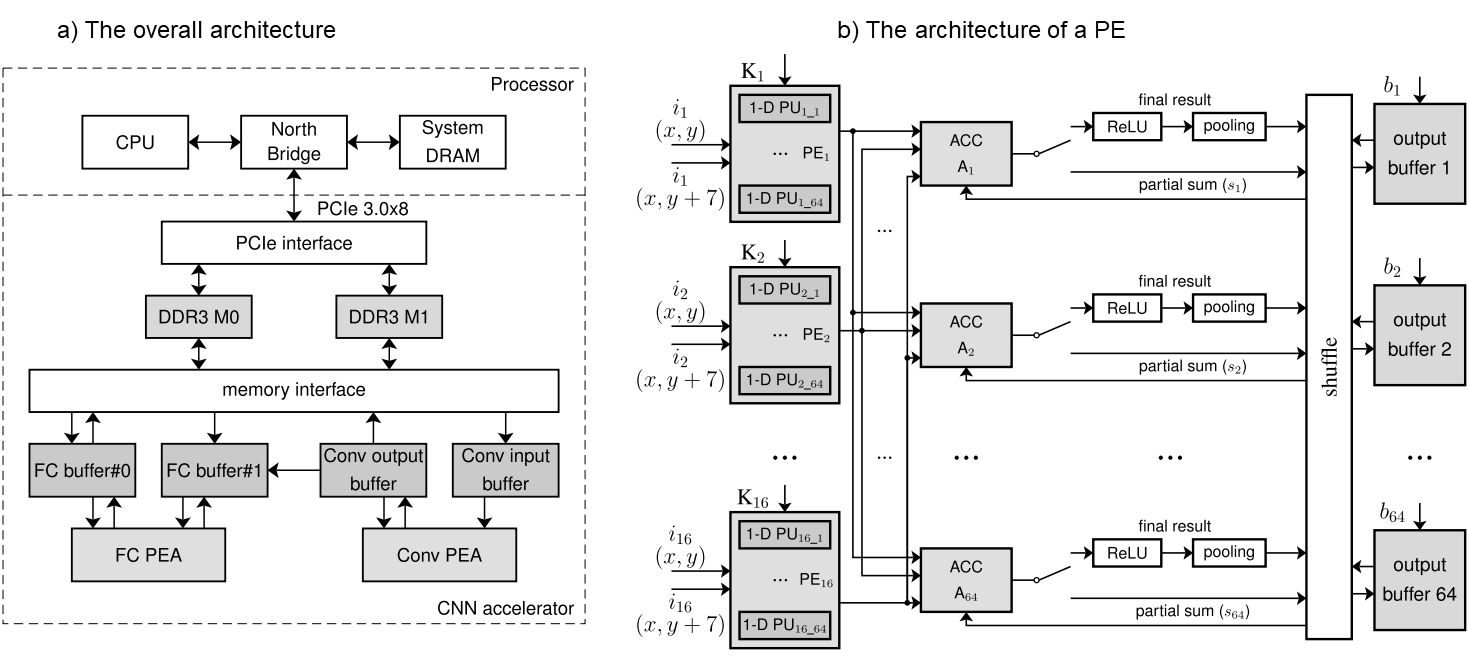
\includegraphics[width=\textwidth]{./figures/3_g.png}
	\caption{(a) System architecture. (b) Processing element array.}
	\label{fig:lian2019high}
\end{figure}
\FloatBarrier

\subsubsection{A 200MHZ 202.4GFLOPS@10.8W VGG16 Accelerator in Xilinx VX690T}
In \cite{mei2017200mhz}, Chunsheng Mei \textit{et al.} presented a hardware accelerator for VGG16 model using half-precision \gls{fp} (16-bit). This design is demonstrated on Xilinx Virtex-7 (XC7VX690T) with PCIe interface. This implementation achieves throughput and power efficiency of \unit[202.4]{GFLOP/s} and \unit[18.72]{GFLOP/s/W}, respectively.

\Fig{fig:mei2017200mhz}(a) presents the block diagram of system architecture. Initially, both the network model and input images are transferred to the on-board DDR3 modules (DDR3 M0 and DDR3 M1) using PCle3.0x8. For forward processing, distinct accelerators are allocated for the convolution and fully-connected layers. An image-grain pipeline is scheduled for both the Fully-Connected Layer Accelerator (FLAcc) and the Convolution Layer Accelerator (CLAcc). While FLAcc processes the fully-connected layers of the current image, CLAcc concurrently processes the convolutional computations for the next image. This heterogeneous architecture is constructed on the condition that the convolution layers are suitable for parallelism, while the fully-connected layer are not. To maximize the use of on-board resources, two sets of CLAcc, Convolution Layer Input Buffer (CLIB), Convolution Layer Output Buffer (CLOB), FLAcc, and Fully-Connected Layer Buffer (FLB) were designed to handle two input images simultaneously. The network parameters are consistently shared between these two system accelerators.

\Fig{fig:mei2017200mhz}(b) shows the CLAcc architecture. The design incorporates two CLAccs, both functionally mirroring each other to process two tasks in tandem. A pingpong storage scheme is utilized for input tiles and kernels, reducing the overhead associated with loading them. Bias parameters are stored in CLOB. When convolution or fully-connected layer operation commences, bias data are taken as the initial accumulation value. Notably, instead of opting for single-precision \gls{fp} (32-bit) arithmetic, the design uses half-precision \gls{fp} (16-bit) arithmetic, which suffices for the VGG16 model accuracy requirements.

Without necessitating network retraining, this design accommodates the model parameters and input maps. Furthermore, the half-precision data format enhances deployment efficiency, reducing off-chip bandwidth and on-chip resources compared to the single-precision format.

\begin{figure}[h!]
	\centering
	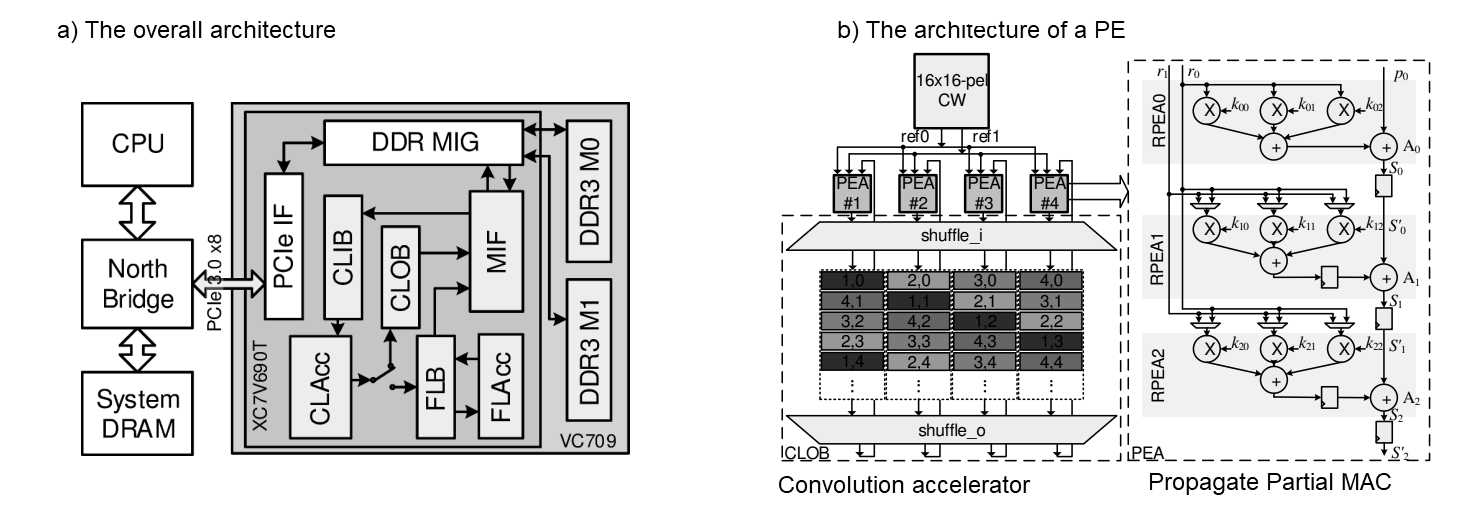
\includegraphics[width=\textwidth]{./figures/1_g.png}
	\caption{(a) System architecture. (b) Convolution accelerator.}
	\label{fig:mei2017200mhz}
\end{figure}
\FloatBarrier

\subsubsection{Low-precision Floating-point Arithmetic for High-performance FPGA-based CNN Acceleration}
In \cite{wu2021low}, Chen Wu \textit{et al.} proposed a low-precision (8-bit) floating-point (LPFP) quantization method for \gls{fpga}-based acceleration. This design is demonstrated on Xilinx Kintex 7 and Ultrascale/Ultrascale+. This implementation achieves throughput and power efficiency of \unit[1086.8]{GOP/s} and \unit[115.4]{GOP/s/W}, respectively.

\Fig{fig:wu2021low}(a) depicts the overarching system architecture. At its core lies the Floating-Point Function Unit (FPFU), containing an array of Processing Elements (PEs). These PEs are designed to compute layer outputs in parallel. Specifically, each PE within the FPFU is optimized to efficiently handle dot-products using the LPFP data format. The on-chip Memory System (MS) incorporates three distinct buffers: the Input Feature Map Buffer (IFMB), Weight Buffer (WB), and Output Feature Map Buffer (OFMB). Utilizing a ping-pong mechanism, these buffers are designed to mitigate the communication latency between on-chip and off-chip memories, a process facilitated by the \gls{dma} module. Additionally, the Central Control Module (CCM) functions as a arbiter for the different modules, translating instructions from the Instruction RAM (IR) into specific signals for associated modules.

\Fig{fig:wu2021low}(b) presents the PE architecture, conceived as a fully pipelined data-flow structure. Upon receiving two vectors, a PE distributes the data among its $N_m$ multipliers. These multipliers then transfer their full precision \gls{fp} results to the Alignment Module (AM). Without truncating any bits, these full precision \gls{fp} products are aligned and transformed into fixed-point numbers. Post alignment, these products are transferred to four fixed-point adder trees, completing four parallel dot-product operations. This simultaneous processing exemplifies the feed-forward mechanism for four pixels across two output channels. The accumulation of partial results (including bias), pooling and activation processes are performed in series inside the Post Process Module (PPM).

\begin{figure}[h!]
	\centering
	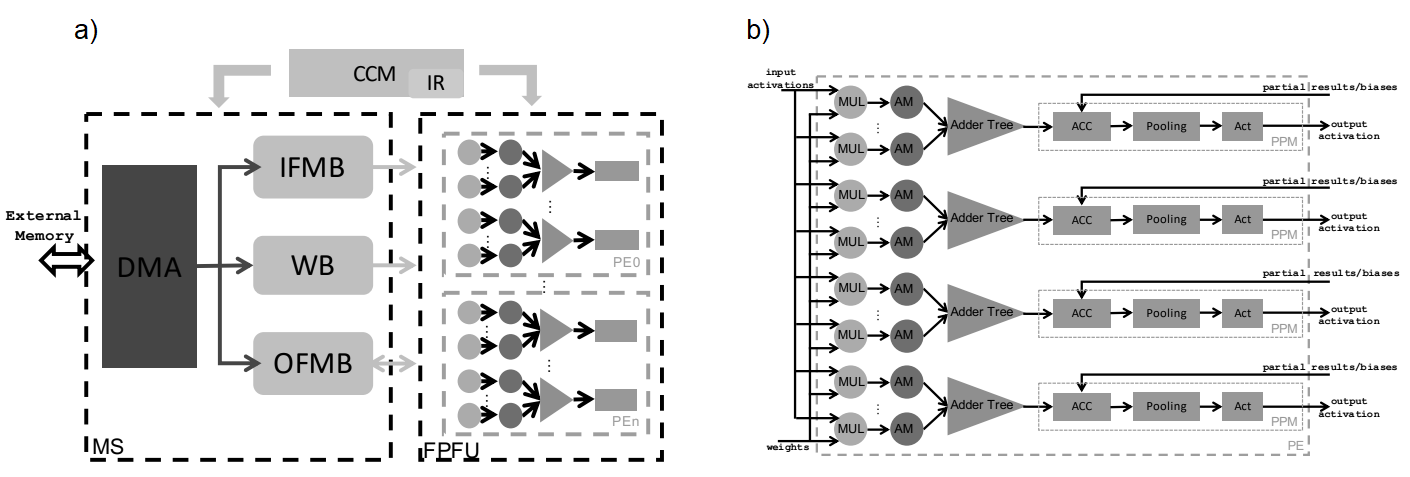
\includegraphics[width=\textwidth]{./figures/2_g.png}
	\caption{(a) System architecture. (b) Processing element.}
	\label{fig:wu2021low}
\end{figure}

\FloatBarrier

\subsubsection{CNN Hardware Acceleration on a Low-Power and Low-Cost APSoC}
In \cite{meloni2019cnn}, Paolo Meloni \textit{et al.} presented a \gls{cnn} inference accelerator for compact and cost-optimized devices. However, this implementation uses fixed-point to process light-weight \gls{cnn} architectures with a power efficiency between \unit[2.49] to \unit[2.98]{GOPS/s/W}.

\Fig{fig:meloni2019cnn}(a) depicts the system architecture, which is a hybrid hardware-software design tailored for the Zynq XC7Z007S \gls{soc}. In this configuration, an ARM Cortex-A9 single-core processor collaborates with a convolution engine situated on the \gls{pl}. This accelerates both compute-bound and memory-bound operations. The \gls{ps} incorporates a memory interface unit, facilitating communication to an off-chip \gls{ddr} memory, which is the storage space for input features, weights, biases, and output features.

\Fig{fig:meloni2019cnn}(b) presents the convolution engine specifics. The compute-intensive convolution operations are handed over to the convolution engine Sum-of-Product (SoP) module, which utilizes 54 \gls{dsp} slices (based on the Xilinx DSP48E1 primitives). The SoP module simultaneously processes three 3x3 weight filters on three input features (denoted as x\_in) acquired by the line buffer. This action determines their cumulative effect on a single output feature. These convolutional partial results are then accumulated using a specialized adder module.

\begin{figure}[h!]
	\centering
	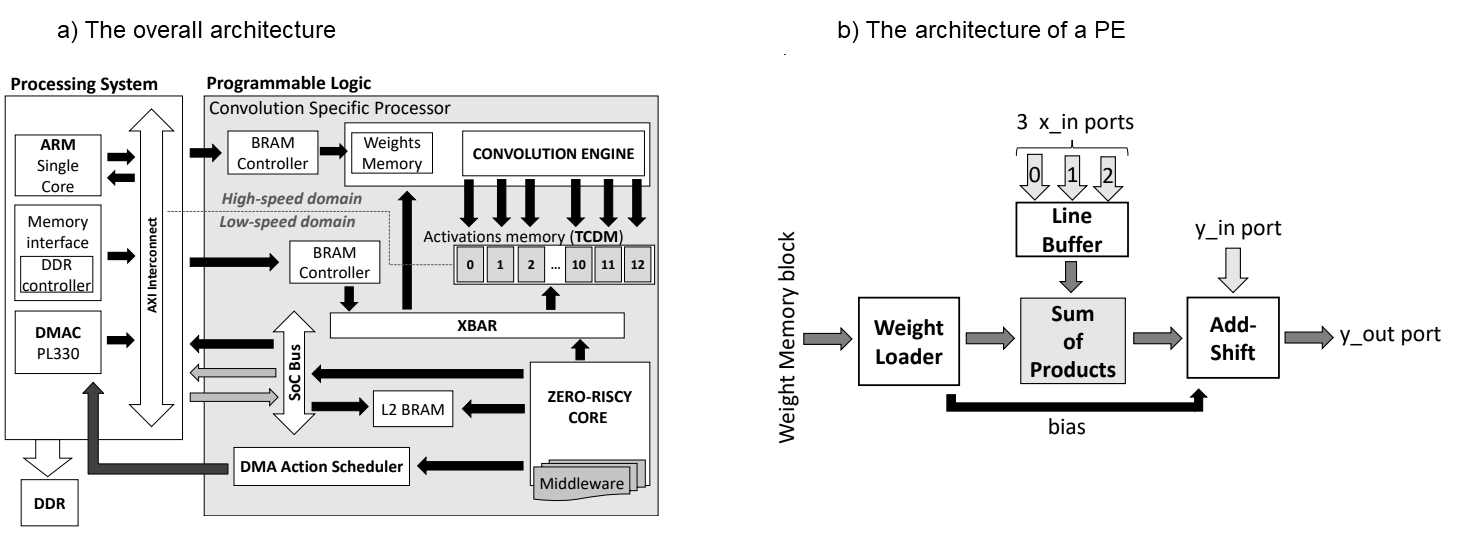
\includegraphics[width=\textwidth]{./figures/4_g.png}
	\caption{(a) System architecture. (b) Convolution engine.}
	\label{fig:meloni2019cnn}
\end{figure}
\FloatBarrier
%%%%%%%%%%%%%%%%%%%%%%%%


\subsection{Neural Network Accelerators for Training and Inference with 8-bit Floating-Point Computation on \gls{asic}
}
State-of-the-art low-power neural network accelerators have demonstrated significant improvements in both energy efficiency and computational performance using 8-bit \gls{fp} arithmetic for training and inference. The studies presented in this subsection uniformly explore the advantages of 8-bit \gls{fp} quantization, specifically with a composition of a 4-bit exponent and 3-bit mantissa for high-accuracy inference, and a 5-bit exponent with a 2-bit mantissa for training.

In \cite{wu2020phoenix}, Chen Wu \textit{et al.} presented proposes the Phoenix architecture implementing 8-bit \gls{fp} quantization. Key findings suggest that this method incurs less error than its fixed-point counterpart. Normalization prior to quantization aids in further error reduction (less than 0.5\% for top-1 and 0.3\%
for top-5 accuracy degradation). Phoenix outperforms other state-of-the-art accelerators when benchmarked with AlexNet and VGG16. The circuit placement and routing results show that Phoenix achieves peak performance of \unit[2.048]{TMAC/s} with \unit[1.44]{mm$^2$} and \unit[1091.2]{mW} at TSMC \unit[28]{nm} technology, respectively. Compared with a state-of-the-art accelerator, Phoenix achieves 3.32$\times$ and 7.45$\times$ better performance with
the same core area for AlexNet and VGG-16, respectively.
Compared with Nvidia TITAN Xp \gls{gpu}, Phoenix consumes
151$\times$ less energy with single image inference.

In \cite{park2021neural}, Jeongwoo Park \textit{et al.} reported an 8-bit \gls{fp} neural network training processor that leverages shared exponent bias (FP8-SEB) for non-sparse neural networks. This implementation uses multiple-way fused multiply-add (FMA) trees for maintaining high numerical precision and reducing energy consumption, demonstrating improved efficiency against conventional neural network training processors. Fabricated in \unit[40]{nm} LP CMOS, the processor consumes
\unit[13.1]{mW} at \unit[0.75]{V}, \unit[20]{MHz} with the maximum energy efficiency of \unit[4.81]{TFLOPS/W}, and \unit[230]{mW} at \unit[1.1]{V}, \unit[180]{MHz} with the maximum performance of \unit[567]{GFLOPS} and area efficiency of \unit[90.7]{GFLOPS/mm$^2$}   .

In \cite{venkataramani2021rapid}, Swagath Venkataramani \textit{et al.} demonstrated a 4-core \gls{ai} chip, called RaPiD, an accelerator that supports various precisions. Notably, the accelerator can handle 16 and 8-bit \gls{fp} computations, as well as 4 and 2-bit fixed-point calculations. Measurements show INT4 inference for batch size of 1 yields 3 - 13.5 (average 7) TOPS/W and FP8 training for a mini-batch of 512 achieves a sustained 102 - 588 (average 203) TFLOPS across a wide range of applications.

Lastly, in \cite{venkataramanaiah202228nm}, Shreyas Kolala Venkataramanaiah \textit{et al.} presented an 8-bit \gls{fp} tensor core-based CNN training processor. This processor incorporates highly parallel tensor cores, ensuring high utilization throughout various phases of the training process. With the integration of dynamic output activation sparsity and other efficiency-enhancing features, this 28nm prototype chip showcases energy efficiency of \unit[16.4]{TFLOPS/W}.



\subsection{Advancements in Neural Network Training: Industrial Research on 8-bit Floating-Point Quantization Techniques}
In the continued pursuit of refining neural network training, the application of 8-bit \gls{fp} quantization -- employing a 5-bit exponent with 2-bit mantissa for training, and a 4-bit exponent with 3-bit mantissa for inference -- has been demonstrated as a common key strategy, as reported by the subsequent studies.

In one of the early explorations into this field, as reported by Michal Gallus \textit{et al.} in \cite{gallus2018handwritten}, 8-bit \gls{fp} numbers were utilized for training the LeNet-5 model for handwritten digit classification achieving $97.10\%$ accuracy (2\% degradation) while reducing space complexity by 75\%. In a study by Naigang Wang \textit{et al.}, referenced in \cite{wang2018training} from IBM T. J. Watson Research Center, the feasibility of using 8-bit \gls{fp} numbers for training deep neural networks was demonstrated. This work introduced innovative techniques such as chunk-based accumulation and \gls{fp} stochastic rounding, showing potential for up to a fourfold increase in throughput on future hardware platforms.

In a notable advancement detailed in \cite{sun2019hybrid} by Xiao Sun \textit{et al.} from IBM T. J. Watson Research Center, the hybrid 8-bit \gls{fp} (HFP8) format was introduced, tailored for a broad spectrum of deep learning applications including image classification and language processing. This format, tested on various architectures such as AlexNet, ResNet, MobileNetV2, DenseNet121, LSTMs, Transformer, MaskRCNN, and SSD-Lite, and datasets like ImageNet, PennTreeBank, WMT14 En-De, SWB300, COCO, and VOC, demonstrated minimal accuracy loss when shifting from baseline FP32 to HFP8 training. Building upon this work, Naveen Mellempudi \textit{et al.}, as reported in \cite{mellempudi2019mixed} from Parallel Computing Lab, Intel Labs, explored a mixed precision training approach. This approach, integrating enhanced loss scaling and stochastic rounding to counteract gradient noise, yielded improved accuracies compared to full precision across various datasets, including ImageNet-1K and WMT16, and a range of models like ResNet-18/34/50, GNMT, and Transformer.

In \cite{liu2021improving}, Fangxin Liu \textit{et al.} adopted a distinct approach by introducing adaptive floating-point (AFP) post-training quantization, which enhances compression rates and inference efficiency without relying on the computationally demanding \gls{qat}. Their work introduces a framework that automatically optimizes and selects the appropriate AFP configuration for each layer, hence maximizing compression effectiveness. This approach results in minimal accuracy degradation (only 0.04\% for ResNet-50 and 0.6\% for MobileNet-v2) compared to their full-precision counterparts.

In conclusion, the adoption of 8-bit floating-point quantization marks a significant advancement in meeting the industry growing demand for compatibility, efficiency, compactness, and precision in neural network training and inference.
\chapter{Accelerating Spike-by-Spike Neural Networks: Hybrid 8-bit Floating-Point and 4-bit Logarithmic Computation} \label{chap.sbs}
\minitoc
\section*{Abstract}
\begin{quote}
In the domain of \glspl{snn}, this chapter explores into the design methodology tailored for low-power inference of \gls{sbs} neural networks in embedded applications. Notably, while \gls{sbs} networks stand out for their reduced model complexity and superior noise robustness compared to conventional \glspl{snn} utilizing the \gls{lif} mechanism, they come with inherent challenges. Particularly, their computational cost and memory footprint have been barriers for deployment on resource-limited devices.

Addressing these challenges, this research capitalizes on the intrinsic error resilience of \gls{sbs} models to improve performance and minimize hardware resources while avoiding model quantization procedures. Central to this approach is the introduction of a novel \gls{mac} module. This module is designed to harmonize computational accuracy and resource efficiency in \gls{fp} operations. This \gls{mac} module provides configurable quality via a hybrid mechanism: it merges standard \gls{fp} representations with a custom 8-bit \gls{fp} format and a 4-bit logarithmic representation. This design excludes the use of a sign bit, which further contributes to the compact and efficient representation of numbers. This design enables the \gls{mac} module to be tailored to the specific resource constraints and performance requirements of a given application. This research makes \gls{sbs} neural networks possible for deployment in resource-constrained environments.
\end{quote}
\section{Introduction}
\label{sec:introduction}
%%% General intro
The exponential improvement in computing performance and the availability of large amounts of data are boosting the use of \gls{ai} applications in our daily lives. Among the various algorithms developed over the years, neural networks have demonstrated remarkable performance in a variety of image, video, audio, and text analytics ~\cite{schmidhuber2015deep,Taigman_2014_CVPR}. 

Historically, \glspl{ann} can be classified into three different generations \cite{Design_Exploration_SbS_Trans20}: the first one is represented by the classical McCulloch and Pitts neuron model using discrete binary values as outputs; the second one is represented by more complex architectures as \gls{mlp} and \gls{cnn} using continuous activation functions; while the third generation is represented by \gls{snn} using spikes as means for information exchange between groups of neurons. Although the \gls{ai} research is currently dominated by \glspl{dnn} from the second generation, the \glspl{snn} belonging to the third generation are receiving considerable attention \cite{Spinnaker_Trans13,ernst2007efficient,Design_Exploration_SbS_Trans20, SNN_Survey_Trans19}.

\glspl{snn} offer advantageous robustness and the potential to achieve power efficiency closer to that of the human brain.
%%%
\glspl{snn} operate reliably using stochastic elements that are inherently non-reliable mechanisms \cite{mcdonnell2011benefits}.
This provides superior resistance against adversary attacks
\cite{ernst2007efficient, Dapello2020.06.16.154542}. Beside
robustness, \glspl{snn} have further advantages like the possibility of a more efficient asynchronous parallelization and higher
energy efficiency than \glspl{dnn}. For
example, Loihi \cite{davies2018loihi}, a \gls{snn} developed by Intel, can
solve LASSO optimization problems with an over three orders of
magnitude better energy-delay product than conventional
approaches. These advantages are motivating large research programs by
major companies (e.g., Intel \cite{davies2018loihi} and IBM
\cite{TrueNorth_Trans15}) as well as pan-european projects in the
domain of spiking neural networks \cite{Spinnaker_Trans13}.


\glspl{snn} emulate the real behavior of neurons in different levels of detail. The more detailed the biological part is emulated, the greater the computational complexity \cite{izhikevich2004model,amunts2019human}. For example, \gls{lif} is a widely used model; however, this model is relatively more complex for emulation in low-power embedded applications.
	
	Alternatively, the \gls{sbs} neural network is a remarkable model for its reduced complexity, which is on the less realistic side of the \gls{snn} scale of biological realism~\cite{rotermund2019Backpropagation,ernst2007efficient}. Consequently, the hardware complexity of \gls{sbs} network implementations is reduced
	\cite{nevarez2020accelerator,rotermund2018massively}. In spite of this, \gls{sbs} still uses stochastic spikes as a means of transmitting information between populations of neurons and thus retains the advantageous robustness of \glspl{snn}.


%%% SbS intro
%SbS neural networks \cite{rotermund2019back,ernst2007efficient} are inspired by the %natural information processing of the mammalian brain.
The conceptual model in \gls{sbs} (see Chapter~\ref{sec:sbs} for a review) differs fundamentally from conventional \glspl{ann} since (a) the building blocks of the network are \glspl{ip_sbs} which are an optimized generative representation with non-negative values, (b) time progresses from one spike to the next, preserving the property of stochastically firing neurons, and (c) a network has only a small number of parameters, which is a noise-robust stochastic version of \gls{nnmf}. The \gls{sbs} network is placed between non-spiking \glspl{nn} and stochastically spiking \glspl{nn}, which offers advantages from both structures \cite{rotermund2019Backpropagation}. On one hand, the \gls{sbs} model incorporates the inherent robustness of \glspl{snn}, which gives the possibility of more efficient asynchronous parallelization and resilience against disturbances based on the synaptic stochasticity; on the other hand, the \gls{sbs} model incorporates the regular flow of information from \glspl{cnn}.  


%%%%%%% Problem statement
As computational demanding algorithms, \glspl{cnn} and \glspl{snn} in particular, must be addressed by specialized hardware architectures. A significant research effort has been performed in \gls{snn} accelerators, see e.g.~\cite{roy2019towards,bouvier2019spiking, young2019review,TrueNorth_Trans15,Spinnaker_Trans13,davies2018loihi}.
  However, hardware accelerators that focus on \gls{sbs} have only been partially investigated so far~\cite{rotermund2018massively}.
  Enhancing \gls{sbs} accelerators will contribute to the deployment of robust neural networks in resource-constrained devices~\cite{nevarez2020accelerator,ernst2007efficient,rotermund2019recurrentsbs, dayan2001theoretical}.

A central point that can be optimized in current \gls{sbs} accelerators
is the use of approximation techniques.
Most \gls{snn} models use \gls{fp}  numerical representation, which imposes high complexity of the required circuits for \gls{fp} operations. Quantization has the potential to improve computational performance; however, this solution is often accompanied by quantization-aware training methods that, in some cases, are problematic or even inaccessible, particularly in deep \gls{snn} algorithms~\cite{zhang2018survey}.

As an alternative, based on the relaxed need for fully precise or deterministic computation of neural networks, approximate computing techniques allow substantial enhancement in processing efficiency with moderated accuracy degradation. Some research papers have shown the feasibility of applying approximate computing to the inference stage of neural networks~\cite{lotrivc2012applicability, sarwar2016multiplier, mrazek2016design, du2014leveraging}. Such techniques usually demonstrated small inference accuracy degradation, but significant enhancement in computational performance, chip-area, and energy consumption. Hence, by taking advantage of the intrinsic error-tolerance of neural networks, approximate computing is positioned as a promising approach for inference on resource-limited devices.

\begin{figure*}[b!]
	\centering
	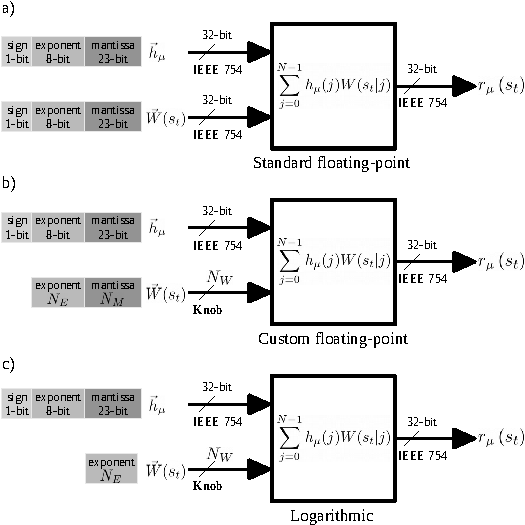
\includegraphics[width=0.5\columnwidth]{./chapters/sbs_accelerator/figures/dot-product_unit.pdf}
	\caption{Dot-product hardware module with (a) standard floating-point (IEEE 754) arithmetic, (b) hybrid custom floating-point approximation, and (c) hybrid logarithmic approximation.}
	\label{fig:dot_product_unit}
\end{figure*}

%%%%%%% Contributions
In this chapter, it is presented an accelerator for \gls{sbs} neural networks with a hardware \gls{mac} unit based on approximate computing with hybrid custom \gls{fp}  and logarithmic number representation. The hardware \gls{mac} unit performs the vector dot-product, which widely used in machine learning algorithms. This hardware unit has a quality configurable scheme based on the exponent and mantissa bit-size of the synaptic-weight vector. \Fig{fig:dot_product_unit} illustrates the \gls{mac} with standard \gls{fp} (IEEE 754) arithmetic, and the proposed approach with hybrid custom \gls{fp}  as well as logarithmic approximation. As a design parameter, the mantissa bit-width of the weight vector provides a tunable knob to trade-off between efficiency and \gls{qor}~\cite{park2009dynamic, han2013approximate}. Since the lower-order bits have smaller significance than the higher-order bits, bit-truncation strategy represents a minor impact on \gls{qor}~\cite{gupta2011impact, mittal2016survey}. Further on, the mantissa bits can be completely removed in order to use only the exponent of a \gls{fp} representation. This configuration becomes a logarithmic representation, which consequently leads to significant architectural-level optimizations using only hardware adders and shifters. Moreover, since approximations and noise have qualitatively the same effect~\cite{venkataramani2015approximate}, it is proposed the noise tolerance plot as an intuitive visual measure to provide insights into the quality degradation and resilience budget of \gls{sbs} networks under approximation effects.

The main contributions presented in this chapter are as follows:

\begin{itemize}
	\item A hardware module for \gls{mac} approximation. To perform the sum of pairwise products of two vectors, this hardware module has the following three design features: (1) the pairwise product is approximated by adding integer exponents and multiplying truncated mantissas, and the sum of products is done by accumulating denormalized integer products with barrel shifters, this increases computational throughput; (2) the synaptic weight vector uses either reduced custom \gls{fp} or logarithmic representation, this reduces memory footprint; and (3) the neuron vector uses either standard or custom \gls{fp} representation, this preserves \gls{qor} and overall inference accuracy.
	\item A hardware design exploration with the proposed dot-product approximation using synaptic weight vectors with custom \gls{fp} and logarithmic representation as shown in \Fig{fig:dot_product_unit}. It is presented the inference run-time, accuracy degradation, resource utilization and power dissipation. Experimental results demonstrate $20.5\times$ run-time enhancement versus embedded CPU (ARM Cortex-A9 at \unit[666]{MHz}), and less than $0.5\%$ of accuracy degradation without retraining on a handwritten digit recognition task (MNIST). This machine learning task simply provides a proof of concept to demonstrate the feasibility of our approximation technique for \gls{sbs} neural network accelerators.
	\item A noise tolerance plot is proposed as quality monitor, which serves as an intuitive visual model to provide insights into the accuracy degradation and noise resilience-budget of \gls{sbs} networks under approximate processing effects.
	\item The present design for dot-product approximation is adaptable as a building block for other error resilient applications (e.g., image/video processing).
\end{itemize}

To promote the research on \gls{sbs} networks, the design exploration framework is made available to the public as an open-source project at:

 \url{https://github.com/YaribNevarez/sbs-framework.git}


\section{Related Work}
\label{sec:related_work}
%%%%%%%%%%%%%%%%%%%%%%%%%%%%%%%%%%%%%%%%%%%%%%%%%%%%%%
For efficient neural network computation, two main optimization strategies are used, namely network compression and classical approximate computing~\cite{bouvier2019spiking}.

\subsection{Network Compression}
Researchers focusing on embedded applications started lowering the precision of weights and activation maps to shrink the memory footprint of the large number of parameters representing \glspl{ann}, a method known as network compression or quantization. This practice takes advantage of the intrinsic error-tolerance of neural networks, as well as their ability to compensate for approximation while training. In this way, reduced bit precision causes a small accuracy loss~\cite{courbariaux2015binaryconnect, han2015deep, hubara2017quantized, rastegari2016xnor}.

In hardware development, \gls{wq} has shown up to $2\times$ improvement in energy consumption with an accuracy degradation of less than $1\%$ \cite{moons20160, whatmough201714}. Some advanced quantization methods yield to \glspl{bnn} allowing the use of \glspl{xnor} instead of the conventional costly \glspl{mac}~\cite{rastegari2016xnor}. In~\cite{sun2018xnor}, Sun et al. report an accuracy of $98.43\%$ on handwritten digit classification (MNIST) with a simple \gls{bnn}. Hence, quantization is a powerful tool for improving the energy efficiency and memory requirements of \gls{ann} accelerators, with limited accuracy degradation.

In addition to quantization, network pruning reduces the model size by removing structural portions of the parameters and its associated computations~\cite{lecun1989optimal,hassibi1992second}. This method has been identified as an effective technique to improve the efficiency of \gls{dnn} for applications with limited computational budget~\cite{molchanov2016pruning,li2016pruning, liu2018rethinking}.

These methods can be used for \glspl{snn} as well. In~\cite{rathi2018stdp}, Rathi et al. report up to $3.1\times$ improvement in energy consumption with an accuracy loss of around $3\%$. Weight quantization allows the designer to realize a trade-off between the accuracy of the \gls{snn} application and efficiency of resources. Approximate computing can also be applied at the neuron level, where irrelevant units are deactivated to reduce the computation cost of the \glspl{snn}~\cite{sen2017approximate}. This computation skipping can be applied randomly on synapses, training \glspl{ann} with stochastic synapses improves generalization, resulting in a better accuracy~\cite{srivastava2014dropout, wan2013regularization}. Such methods are compatible with \glspl{snn} and have been tested both during training~\cite{neftci2016stochastic, srinivasan2016magnetic} and operation \cite{buesing2011neural}, and even to define the connectivity between layers \cite{bellec2017deep, chen20184096}. Implementations of spiking neuromorphic systems in \gls{fpga}~\cite{sheik2016synaptic} and hardware~\cite{jerry2017ultra} demonstrated that synaptic stochasticity allows to increase the final accuracy of the networks while reducing memory footprint.

Quantization is therefore a powerful technique to improve energy efficiency and memory requirements of \gls{ann} and \gls{snn} accelerators, with small accuracy degradation. However, this approach requires quantization-aware training methods that, in some cases, are problematic or even inaccessible, particularly in emerging deep \gls{snn} algorithms~\cite{zhang2018survey}.

\subsection{Classical Approximate Computing}
Approximate computing has been used in a wide range of applications to increase the computational efficiency in hardware~\cite{han2013approximate}. This approach consists of designing processing elements that approximate their computation by employing modified algorithmic logic units~\cite{han2013approximate}. In~\cite{kim2013energy}, Kim et al. have shown \glspl{snn} using carry skip adders achieving $2.4\times$ latency enhancement and $43\%$ more energy efficiency, with an accuracy degradation of 0.97\% on a handwritten digit classification task (MNIST). Therefore, approximate computing provides important enhancement in energy efficiency and processing speed.

However, as the complexity of the dataset increases, as well as the depth of the network topology, such as ResNet~\cite{he2016deep} on ImageNet~\cite{russakovsky2015imagenet}, the accuracy degradation becomes more important and may not be negligible anymore~\cite{rastegari2016xnor}, especially for critical applications such as autonomous driving. Therefore, it is not certain that network compression techniques and approximate computing are suitable for all applications.

\subsection{Spike-by-Spike Neural Networks Accelerators}
Rotermund et al. demonstrated the feasibility of a neuromorphic \gls{sbs} \gls{ip_sbs} on a Xilinx Virtex 6 \gls{fpga}~\cite{rotermund2018massively}. It provides a massively parallel architecture, optimized to reduce memory access and suitable for \gls{asic} implementations. Nonetheless, this design is considerably resource-demanding if implemented as a full \gls{sbs} network in today's embedded technology.
%%%%%%%%%%%%%%%%%%%%%%%%%%%%%%%%%%%%%%%%%%%%%%%%%%%%%%
\section{System Design}
\label{sec:system_design}

	In this section, it is presented a hardware architecture composed of specialized heterogeneous \glspl{pu} with hybrid custom floating-point and logarithmic dot-product approximation. This approach represents an advantageous design for error resilient applications in resource-constrained devices due to the reduced hardware utilization and memory footprint. Furthermore, the proposed approach allows the implementation of stationary synaptic weight matrices as internal accelerator storage based on the reduced memory footprint.
	

Regarding the software architecture, this is structured as a
layered object-oriented application framework written in the C programming language. This offers a comprehensive high level embedded software \gls{api} that allows the construction of scalable sequential \gls{sbs} networks with configurable hardware acceleration. Conceptually this design is modular, reusable, and extensible. The overall structure is depicted in \Fig{fig:sbs_sw_stack}.

\begin{figure*}[b!]
	\centering
	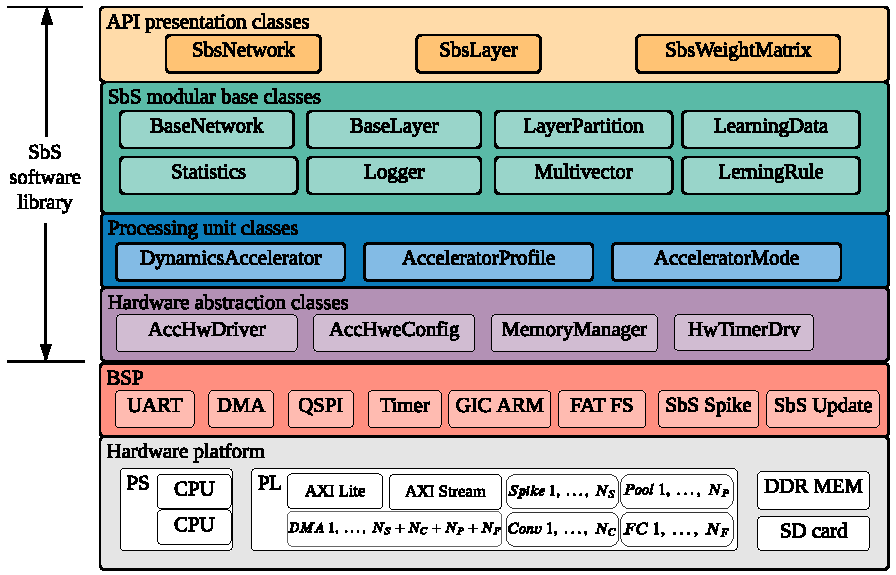
\includegraphics[width=0.5\columnwidth]{./chapters/sbs_accelerator/figures/sbs_software_component.pdf}
	\caption{System-level overview of the embedded software architecture.}
	\label{fig:sbs_sw_stack}
\end{figure*}

\subsection{Hardware Architecture} \label{Hardware_architecture}
As a hardware/software co-design, the system architecture is an embedded \gls{cpu}+\gls{fpga}-based platform, where the acceleration of \gls{sbs} network computation is based on asynchronous\footnote{The system is synchronous at the circuit level, but the execution is asynchronous in terms of jobs.} execution of parallel heterogeneous processing units: \emph{Spike} (input layer), \emph{Conv} (convolution), \emph{Pool} (pooling), and \emph{FC} (fully connected). \Fig{fig:hw_sbs} illustrates the system overview as a scalable structure. For hyperparameter configuration, each \gls{pu} uses AXI-Lite interface. For data transfer, each \gls{pu} uses AXI-Stream interfaces via \gls{dma} allowing data movement with high transfer rate. Each \gls{pu} asserts an interrupt flag once the job or transaction is complete. This interrupt event is handled by the embedded \gls{cpu} to collect results and start a new transaction.

The hardware architecture can resize its resource utilization by changing the number of \gls{pu} instances prior to the hardware synthesis, this provides scalability with a good trade-off between area and throughput. The dedicated \glspl{pu} for \emph{Conv} and \emph{FC} implement the proposed dot-product approximation as a system component. The \glspl{pu} are written in System C using Xilinx Vivado \gls{hls}. In this research, we illustrate the integration of the approximate dot-product component on the \emph{Conv} \gls{pu}.

\begin{figure*}[b!]
	\centering
	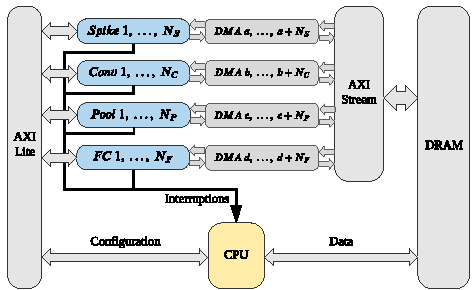
\includegraphics[width=0.5\columnwidth]{./chapters/sbs_accelerator/figures/sbs_hw.pdf}
	\caption{System-level hardware architecture with scalable number of heterogeneous \glspl{pu}: \emph{Spike}, \emph{Conv}, \emph{Pool}, and \emph{FC}}
	\label{fig:hw_sbs}
\end{figure*}

\subsection{Conv Processing Unit}
This hardware module computes the dynamics of the \gls{ip_sbs} defined by \Equ{eq:sbs_update} and offers two modes of operation: \emph{configuration} and \emph{computation}.

\subsubsection{Configuration Mode}
In this mode of operation, the \gls{pu} receives and stores in on-chip memory (BRAM) the hyperparameters to compute the \gls{ip_sbs} dynamics: $\epsilon$ as the epsilon, $N$ as the length of $\vec{h}_\mu\in\mathbb{R}^{N}$, $K\in\mathbb{N}$ as the size of the convolution kernel, and $H\in\mathbb{N}$ as the number of \glspl{ip_sbs} to process per transaction. $H$ is the number of \glspl{ip_sbs} forming a layer or a partition.

Additionally, the processing unit also stores in on-chip memory (BRAM) the synaptic weight matrix using a number representation with a reduced memory footprint. Fundamentally, the synaptic weight matrix is defined by $W\in\mathbb{R}^{K\times K\times M\times N}$ with $0\le W(s_t|j)\le1$ and $\sum_{s_t=0}^{M-1}W(s_t|j)=1$ \cite{rotermund2019Backpropagation}. Hence, $W$ employs only positive normalized real numbers. Therefore, $W$ is deployed using a reduced floating-point or logarithmic representation as follows:

\begin{itemize}
	\item{Custom floating-point representation}.
	In this case, $W$ is deployed with a reduced floating-point representation using the designer defined bit-width for the exponent and for the mantissa. For example, 4-bit exponent, 1-bit mantissa; as a result: 5-bit custom floating-point. The proposed method to determine the required bit-width is described in Section~{\ref{sec:dot-product_hardware_module}}.
	\item{Logarithmic representation}.
	In this case, the synaptic weight matrix is $W\in\mathbb{N}^{K\times K\times M\times N}$ with positive natural numbers. Since $0\le W(s_t|j)\le1$ and $\sum_{s_t=0}^{M-1}W(s_t|j)=1$, $W$ has only negative values in the logarithmic domain. Hence, the sign bit is omitted, and the values are represented as natural numbers. Therefore, $W$ is deployed with a representation using the necessary bit-width for the exponent according to the given application. For example, 4-bit exponent. The method to determine the required bit-width is described in Section~{\ref{sec:dot-product_hardware_module}}.
\end{itemize}

In order to deploy different \gls{sbs} models, the \emph{Conv} processing units can load different hyperparameters and synaptic weight matrices as required via the embedded software.

\subsubsection{Computation Mode}
In this mode of operation, the \gls{pu} executes a transaction to process a group of \glspl{ip_sbs} using the previously given hyperparameters and synaptic weight matrix. This process operates in six stages as shown in \fig{fig:hw_conv}. In the first two stages, the \gls{pu} receives $\vec{h}_\mu\in\mathbb{R}^{N}$, then the \gls{pu} calculates the emitted spike and stores it in $S^{new}\in\mathbb{N}^{H}$ (output spike vector). From the third to the fifth stage, the \gls{pu} receives $S_t\in\mathbb{N}^{K\times K}$ (input spike matrix), then it computes the update dynamics, and then it dispatches $\vec{h}_\mu^{new}\in\mathbb{R}^{N}$ (updated \gls{ip_sbs}). This process repeats for $H$ number of loops (for each \gls{ip_sbs} of the layer or partition). Finally, $S^{new}$ is dispatched.

The computation of the update dynamics (see \fig{fig:hw_conv}(d)) operates in two stages or hardware modules: \emph{dot-product} and \emph{neuron update}. First, the \emph{dot-product} module calculates the sum of pairwise products of $\vec{h}_{\mu}$ and $\vec{W}(s_t)$, each pairwise product is stored as intermediate results. Subsequently, the \emph{neuron update} module calculates \equ{eq:sbs_update} reusing parameters and previous intermediate results.


The calculation of the dot-product of \equ{eq:sbs_update} represents a considerable computational cost using standard floating-point in non-quantized network models. Fortunately, the pair product of $h_{\mu}(j)$ and $W(s_t|j)$ was defined by us as an approximable factor in the dot-product of \equ{eq:sbs_update}. In the following section, we focus on an optimized dot-product hardware design based on approximate computing.


\begin{figure*}[b!]
	\centering
	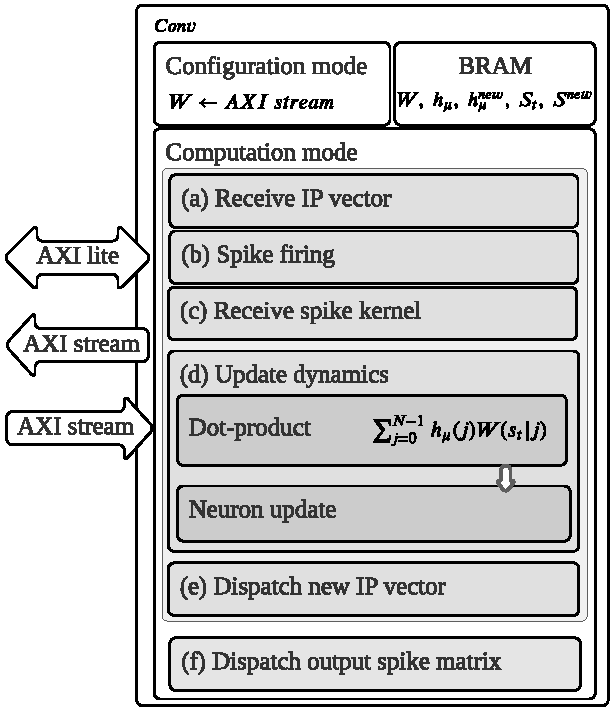
\includegraphics[width=0.5\columnwidth]{./chapters/sbs_accelerator/figures/sbs_conv.pdf}
	\caption{The \emph{Conv} processing unit and its six stages: (a) receive \gls{ip_sbs} vector, (b) spike firing, (c) receive spike kernel, (d) update dynamics, (e) dispatch new \gls{ip_sbs} vector, (f) dispatch output spike matrix.}
	\label{fig:hw_conv}
\end{figure*}

\subsection{Dot-Product Hardware Module}
\label{sec:dot-product_hardware_module}
The dot-product hardware module is part of an application-specific architecture optimized to approximate the dot-product of arbitrary length vectors, see \equ{eq:dot_product}. For quality configurability, we parameterized the mantissa bit-width of $\vec{W}(s_t)$, which provides a tunable trade-off between resource utilization and \gls{qor}. Since the lower-order bits have smaller significance than the higher-order bits, removing them may have only a minor impact on \gls{qor}. We designate this as hybrid custom floating-point approximation (see {\fig{fig:dot_product_unit}}(b)).

\begin{eqnarray} \label{eq:dot_product}
r_{\mu}\left(s_t\right)=\sum_{j=0}^{N-1}h_{\mu}(j)W(s_t|j)
\end{eqnarray}

Further on, we remove the mantissa bits completely in order to use only the exponent of a floating-point representation. Hence, the worst-case quality and yet the most efficient configuration becomes a logarithmic representation. Consequently, this structure leads to advantageous architectural optimizations using only adders and barrel shifters for dot-product approximation in hardware. We designate this as hybrid logarithmic approximation (see {\fig{fig:dot_product_unit}}(c)).

In order to determine the required bit-width for the number representation, we use {\equ{eq:exp_max}}, {\equ{eq:bits_exp}}, and {\equ{eq:bits_bitwidth}}.

\begin{eqnarray} \label{eq:exp_max}
E_{\min}=\log _2(\min_{\forall i}(W(i)))
\end{eqnarray}

\begin{eqnarray} \label{eq:bits_exp}
N_E=\lceil\log_2(|E_{\min}|)\rceil
\end{eqnarray}

\begin{eqnarray} \label{eq:bits_bitwidth}
N_W=N_E + N_M
\end{eqnarray}


The \equ{eq:exp_max} obtains the exponent of the minimum entry value in the synaptic weight matrix. Since $0\le W(s_t|j)\le1$ and $\sum_{s_t=0}^{M-1}W(s_t|j)=1$, $W$ has only negative values in the logarithmic domain; the smallest value is expressed by the biggest negative exponent ($E_{\min}$). Then, the {\equ{eq:bits_exp}} obtains the necessary bit-width to represent the exponent ($N_E$). Finally, we obtain the total bit-width by incorporating both exponent and mantissa bit-widths in {\equ{eq:bits_bitwidth}}. $N_M$ denotes the mantissa bit-width, this is a knob parameter that is tuned by the designer to trade-off between resource utilization and \gls{qor}. The bit-width concept is illustrated in {\fig{fig:dot_product_unit}}.

In this section, we will present three pipelined hardware modules with standard floating-point (IEEE 754) computation, hybrid custom floating-point approximation, and hybrid logarithmic approximation.

\subsubsection{Dot-Product with Standard Floating-Point Computation}
 The hardware module to calculate the dot-product with standard floating-point computation is shown in \Fig{fig:dot_product_float}. This diagram presents the hardware blocks and their clock cycle schedule. This module loads both $h_\mu(j)$ and $W(s|j)$ from BRAM, then the \gls{pu} executes the pairwise product (\Fig{fig:dot_product_float}(c)) and accumulation (\Fig{fig:dot_product_float}(d)). Intermediate results of $h_\mu(j) W(s_t|j)$ are stored in BRAM for reuse in the neuron update stage. The latency in clock cycles of this hardware module is defined by \Equ{eq:dot_standard_float_latency}, where $N$ is the vector length of the dot-product. This equation is obtained from the general pipelined hardware latency formula: $L=\left(N-1\right)II+IL$, where $II$ is the initiation interval (\Fig{fig:dot_product_float}(a)), and $IL$ is the iteration latency (\Fig{fig:dot_product_float}(b)). Both $II$ and $IL$ are obtained from the high-level synthesis analysis. The equation for the latency with standard 32-bit floating-point is:
 \begin{eqnarray} \label{eq:dot_standard_float_latency}
 L_{f32}=10N+9
 \end{eqnarray}
 
In this design, the high-level synthesis tool infers computational blocks with considerable latency cost for standard floating-point. In the case of floating-point multiplication (\Fig{fig:dot_product_float}(c)), the synthesis infers a hardware block with a latency cost of 5 clock cycles. This block executes addition of exponents, multiplication of mantissas, and mantissa correction (when needed). Moreover, in the case of floating-point addition (\ref{fig:dot_product_float}(d)), the synthesis infers a hardware block with a latency cost of 9 clock cycles. Seemingly, this block executes alignment of mantissas, addition, and correction (when needed). Therefore, the use of standard floating-point results in high computational cost, this represents unnecessary overhead in error tolerant applications.


\begin{figure*}[b!]
	\centering
	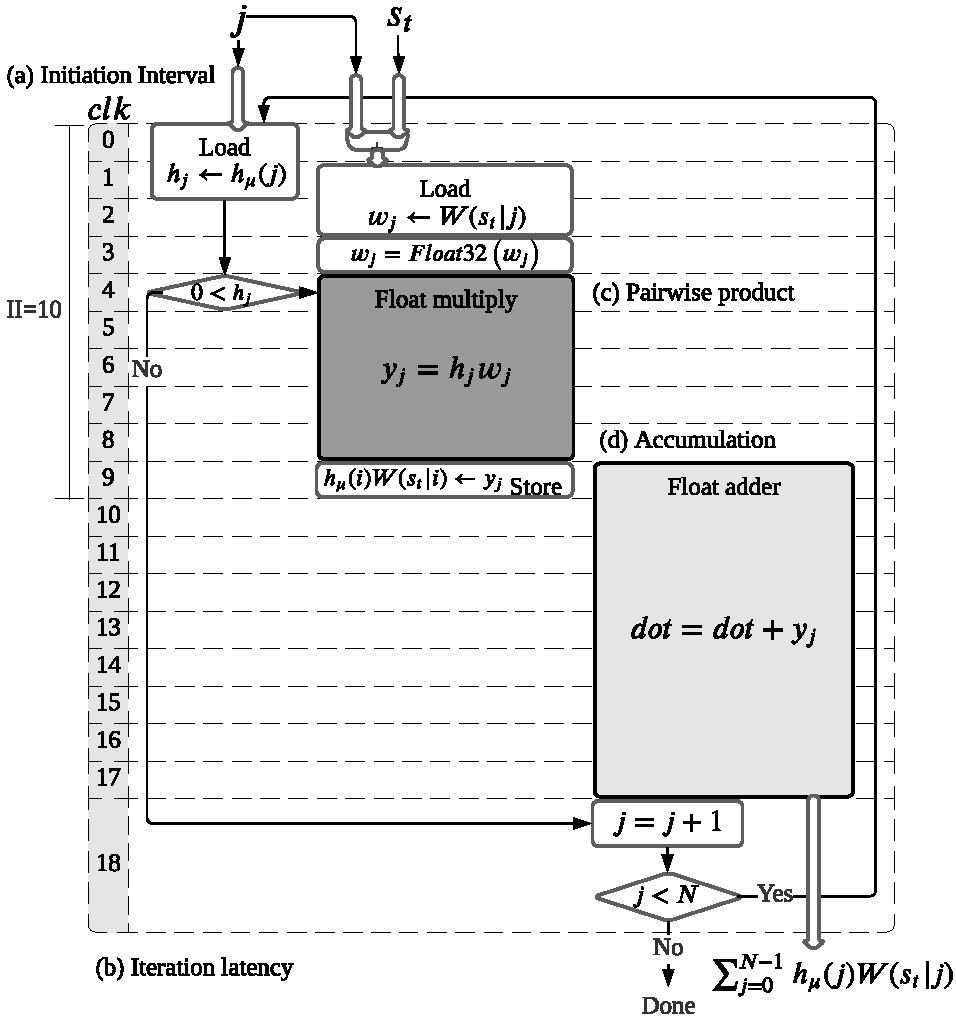
\includegraphics[width=0.5\columnwidth]{./chapters/sbs_accelerator/figures/dot_product_float.pdf}
	\caption{Dot-product hardware module with standard floating-point (IEEE 754) computation, (a) exhibits the initiation interval of 10 clock cycles, (b) presents the iteration latency of 19 clock cycles, (c) shows the pairwise product block in dark-gray, and (d) illustrates the accumulation block in light-gray.}
	\label{fig:dot_product_float}
\end{figure*}

\subsubsection{Dot-Product with Hybrid Custom Floating-Point and Logarithmic Computation}
 The hardware module to calculate dot-product with hybrid custom floating-point approximation is shown in \Fig{fig:dot_product_custom}. In this design, $h_\mu(j)$ uses standard 32-bit floating-point number representation, and $W(s|j)$ uses a positive reduced custom floating-point number representation, where the mantissa bit width is the quality configurability knob. This parameter is tuned by the designer to trade-off between QoR and resource utilization, thus, energy consumption.
 
 \begin{figure*}
 	\centering
 	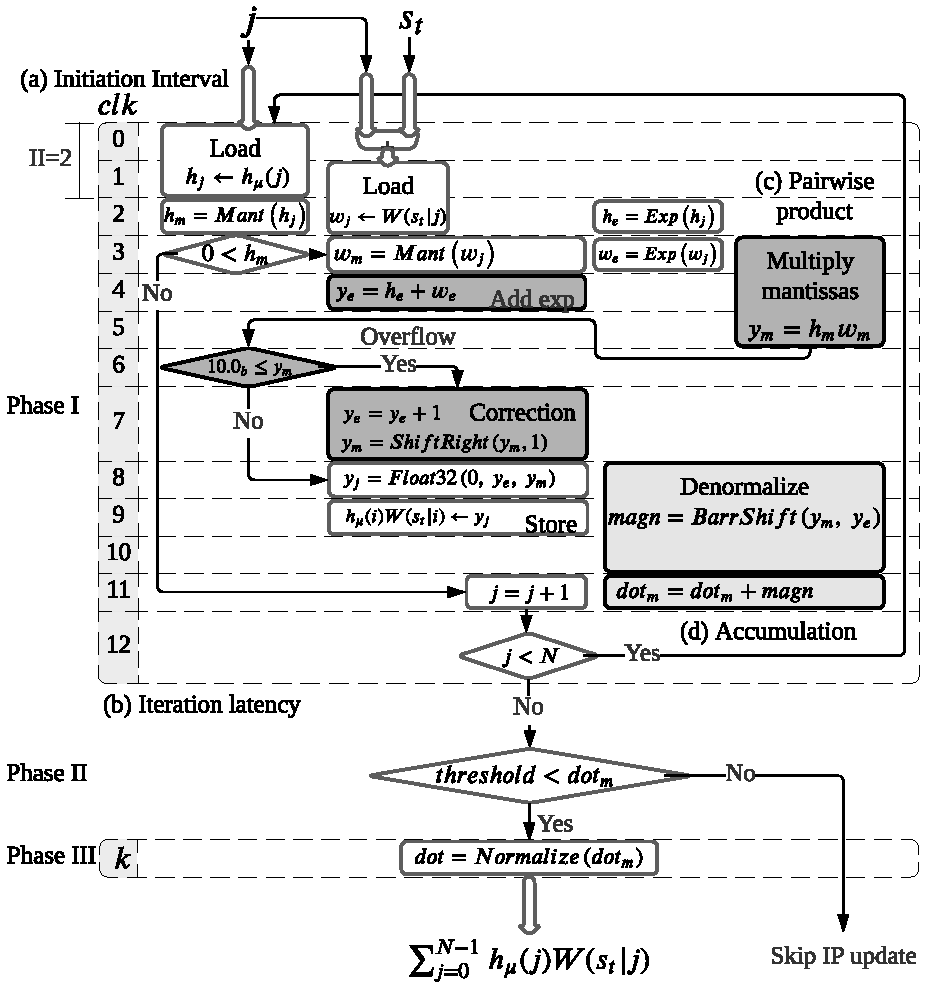
\includegraphics[width=0.5\columnwidth]{./chapters/sbs_accelerator/figures/dot_product.pdf}
 	\caption{Dot-product hardware module with hybrid custom floating-point approximation, (a) exhibits the initiation interval of 2 clock cycles, (b) presents the iteration latency of 13 clock cycles, (c) shows the pairwise product blocks in dark-gray, and (d) illustrates the accumulation blocks in light-gray.}
 	\label{fig:dot_product_custom}
 \end{figure*}
 
 As the most efficient setup, by completely truncating the mantissa of $W(s|j)$ leads to a slightly different hardware architecture using only adders and shifters, which computes the dot-product with hybrid logarithmic approximation. This is shown in \Fig{fig:dot_product_log}.
 
  \begin{figure*}
 	\centering
 	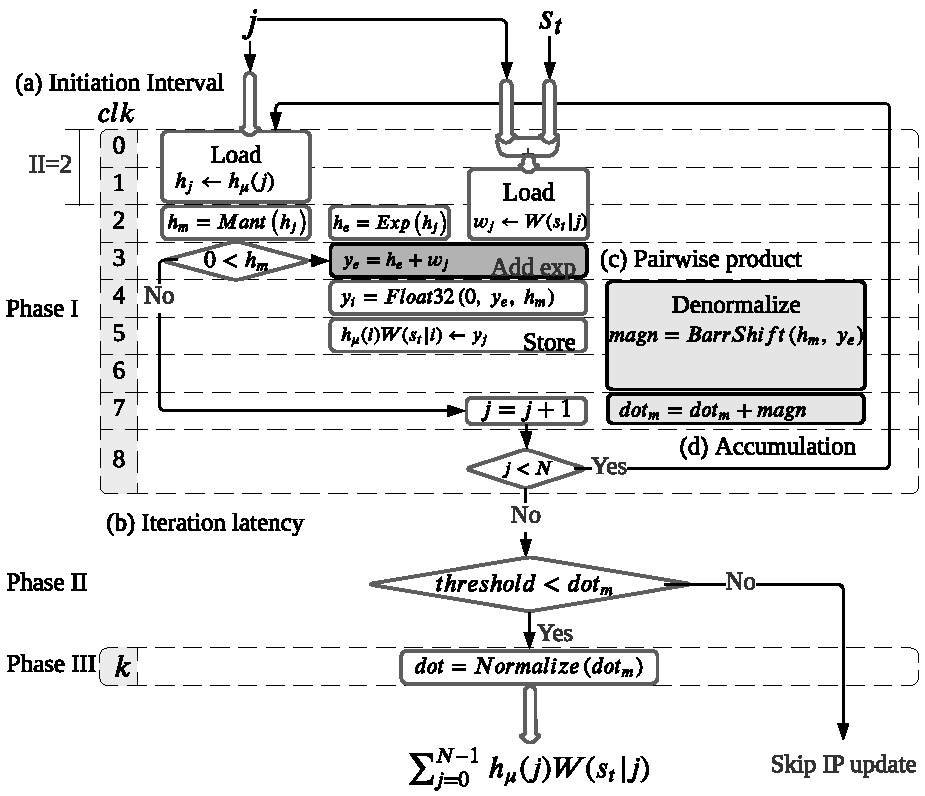
\includegraphics[width=0.5\columnwidth]{./chapters/sbs_accelerator/figures/dot_product_log.pdf}
 	\caption{Dot-product hardware module with hybrid logarithmic approximation, (a) exhibits the initiation interval of 2 clock cycles, (b) presents the iteration latency of 9 clock cycles, (c) shows the pairwise product block in dark-gray, and (d) illustrates the accumulation blocks in light-gray.}
 	\label{fig:dot_product_log}
 \end{figure*}
 
Additionally, the exponent bit-width of $W(s|j)$ is a design parameter for efficient resource utilization and it is defined based on the application and deployment needs.
 
 The hybrid custom floating-point and logarithmic approximation designs work in three phases: \emph{Computation}, \emph{Threshold-test}, and \emph{Result normalization}.
 
 \begin{itemize}
 	\item{Phase I, \emph{Computation}}: 
 	\\This phase approximates the magnitude of the dot-product in a denormalized representation. This is calculated in two iterative steps over each vector element: \emph{pairwise product} and \emph{accumulation}. \emph{Pairwise product} is executed either in hybrid custom floating-point or hybrid logarithmic approximation described below.
 	 \begin{itemize}[label={--}]
 	 	\item{Pairwise product}.
 	 	\begin{itemize} [label={--}]
	 		\item{Hybrid custom floating-point approximation}.
	 	 	As shown in \Fig{fig:dot_product_custom}(c) in dark-gray, the pairwise product is approximated by adding exponents and multiplying mantissas of $W(s|i)$ and $h_\mu(i)$. If the mantissa multiplication results in an overflow, then it is corrected by increasing the  exponent and shifting the resulting mantissa by one position to the right. Then, as intermediate result, $h_\mu(j) W(s_t|j)$ is stored for future reuse in the neuron update calculation. In this design, the pairwise product has a latency of 5 clock cycles.
	 	 	\item{Hybrid logarithmic approximation}.
	 	 	As shown in \Fig{fig:dot_product_log}(c) in dark-gray, the pairwise product is approximated by adding $W(s|i)$ to the exponent of $h_\mu(i)$, since the values of $W(s|j)$ are represented in the logarithmic domain and $h_\mu(j)$ in standard floating-point. In this design, the pairwise product has a latency of one clock cycle.
 	 	\end{itemize}
 		\item{Accumulation}. As shown in both \Fig{fig:dot_product_custom}(d) and \Fig{fig:dot_product_log}(d) in light-gray, first, it is obtained the denormalized representation of $h_\mu(j) W(s_t|j)$ by shifting its mantissa using its exponent as shifting parameter (barrel shifter). Then, this denormalized representation is accumulated to obtain the approximated magnitude of the dot-product.
 	 \end{itemize}
 	The process of pairwise product and accumulation iterates over each element of the vectors. The computation latency is given by \Equ{eq:dot_standard_custom_float_latency} for hybrid custom floating-point, and \Equ{eq:dot_log_latency} for hybrid logarithmic, where $N$ is the length of the vectors. Both pipelined hardware modules have the same throughput, since both have two clock cycles as initiation interval. 	
 	\begin{eqnarray} \label{eq:dot_standard_custom_float_latency}
 	L_{custom}=2N+11
 	\end{eqnarray} 	
	\begin{eqnarray} \label{eq:dot_log_latency}
 	L_{log}=2N+7
 	\end{eqnarray}
 	
 	\item{Phase II, \emph{Threshold-test}}: \\
	The accumulated denormalized magnitude is tested to be above of a predefined threshold, it must be above zero, since the dot-product is the denominator in \Equ{eq:sbs_update}.
 	If passing the threshold, then the next phase is executed. Otherwise the rest of update dynamics is skipped. The threshold-test takes one clock cycle.
 	\item{Phase III, \emph{Result-normalization}}: \\
 	In this phase, the dot-product is normalized to obtain the exponent and mantissa in order to convert it to standard floating-point for later use in the neuron update. The normalization is obtained by shifting the approximated dot-product magnitude in a loop until it is in the form of a normalized mantissa where the iteration count represents the exponent of the dot-product. Each iteration takes one clock cycle.
 	
 \end{itemize}

The total latency of the hardware module with hybrid custom floating-point and hybrid logarithmic approximation is the accumulated latency of the three phases.

The proposed architectures with approximation approach exceeds the performance of the design with standard floating-point. This performance enhancement is achieved by decomposing the floating-point computation into an advantageous handling of exponent and mantissa using intermediate accumulation in a denormalized representation and only one final normalization.



\section{Experimental Results}
\label{sec:experimental_results}
The proposed architecture is demonstrated on a Xilinx Zynq-7020. This device integrates a dual ARM Cortex-A9 based \gls{ps} and \gls{pl} equivalent to Xilinx Artix-7 (\gls{fpga}) in a single chip \cite{xilinx2015zynq}. The Zynq-7020 architecture conveniently maps the custom logic and software in the \gls{pl} and \gls{ps} respectively as an embedded system.

In this platform, the proposed hardware architecture is implemented to deploy the \gls{sbs} network structure shown in \ref{fig:sbs_network} for handwritten digit classification task for MNIST data set. The \gls{sbs} model is trained using standard floating-point. Matlab software is used for this \gls{sbs} network implementation. The resulting synaptic weight matrices are deployed on the embedded system as binary files stored in a micro SD memory card. In the embedded software, the \gls{sbs} network is built as a sequential model using the \gls{api} from the \gls{sbs} embedded software framework \cite{nevarez2020accelerator}. This \gls{api} allows to configure the computational workload of the neural network, this can be distributed among the hardware processing units and the embedded \gls{cpu}.

For the evaluation of this approach, it is presented a design exploration by reviewing the computational latency, inference accuracy, resource utilization, and power dissipation. First, the performance of the embedded \gls{cpu} is taken as benchmark, and then repeat the measurements on hardware processing units with standard floating-point computation. Afterwards, the dot-product architecture is evaluated addressing a design exploration with hybrid custom floating-point approximation, as well as the hybrid logarithmic approximation. Finally, a discussion of results is presented.


\subsection{Performance Benchmark}
\subsubsection{Benchmark on Embedded CPU}

The performance of the \gls{cpu} for \gls{sbs} network inference is examined. In this case, the embedded software builds the \gls{sbs} network as a sequential model mapping the entire computation to the \gls{cpu} (ARM Cortex-A9) at \unit[666]{MHz} and a power dissipation of \unit[1.658]{W}.

The \gls{sbs} network computation on the \gls{cpu} reaches a latency of \unit[34.28]{ms} per spike with accuracy of \unit[99.3]{\%} correct classification on the $10,000$ image test set with $1000$ spikes. The latency and schedule of the \gls{sbs} network computation are displayed in \Tab{tab:latency_sw} and \Fig{fig:latency_sw}, respectively.

\begin{table}[!t]\centering
	\caption{Computation on embedded CPU.}\label{tab:latency_sw}
	\scriptsize
\begin{tabular}{lrr}\toprule
	\textbf{Layer} &\textbf{Latency (ms)} \\\midrule
	HX\_IN &1.184 \\
	H1\_CONV &4.865 \\
	H2\_POOL &3.656 \\
	H3\_CONV &20.643 \\
	H4\_POOL &0.828 \\
	H5\_FC &3.099 \\
	HY\_OUT &0.004 \\
		
	TOTAL &34.279 \\
	\bottomrule
\end{tabular}
\end{table}

\begin{figure*}[b!]
	\centering
	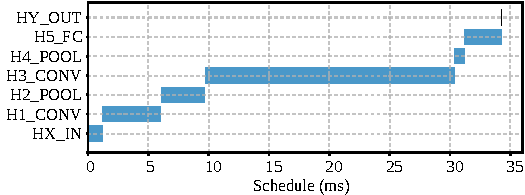
\includegraphics[width=0.5\columnwidth]{./chapters/sbs_accelerator/figures/latency_sw.pdf}
	\caption{Computation on embedded CPU.}
	\label{fig:latency_sw}
\end{figure*}

\subsubsection{Benchmark on Processing Units with Standard Floating-Point Computation}
The system architecture shown in \Fig{fig:hw_sbs_8_pu} is implemented to benchmark the computation on hardware \glspl{pu} with standard floating-point. The embedded software builds the \gls{sbs} network as a sequential model and delegates the network computation to the hardware processing units at \unit[200]{MHz} as clock frequency.

\begin{figure*}[b!]
	\centering
	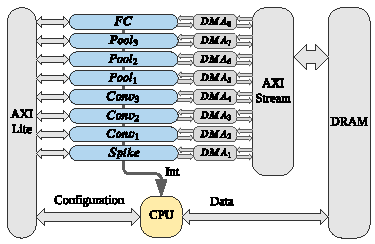
\includegraphics[width=0.5\columnwidth]{./chapters/sbs_accelerator/figures/sbs_hw_experimental.pdf}
	\caption{System overview of the top-level architecture with 8 processing units.}
	\label{fig:hw_sbs_8_pu}
\end{figure*}

The layers of the neural network with the most neurons are partitioned for asynchronous parallel processing. Since \emph{H2\_POOL} and \emph{H3\_CONV} are the layers with the most neurons, the computational workload is distributed between two \glspl{pu} for each one of these layers. The output layer \emph{HY\_OUT} is fully processed by the \gls{cpu}, since it is the layer with fewest neurons. The hardware mapping and the computation schedule of this deployment are displayed in \Tab{tab:latency_fp} and \Fig{fig:latency_pu_fp}, respectively.

\begin{table}[!t]\centering
	\caption{Performance of processing units with standard floating-point (IEEE 754) computation.}\label{tab:latency_fp}
	\scriptsize
	\begin{tabular}{llrrrrrr}\toprule
		\multicolumn{2}{c}{\textbf{Hardware mapping}} & &\multicolumn{4}{c}{\textbf{Computation schedule (ms)}} \\\cmidrule{1-2}\cmidrule{4-7}
		\textbf{Layer} &\textbf{PU} & &$t_s$ &$t_{CPU}$ &$t_{PU}$ &$t_f$ \\\midrule
		HX\_IN &Spike & &0 &0.056 &0.370 &0.426 \\
		H1\_CONV &Conv1 & &0.058 &0.598 &2.002 &2.658 \\
		\multirow{2}{*}{H2\_POOL}
		&Pool1 & &0.658 &0.126 &1.091 &1.875 \\
		&Pool2 & &0.785 &0.125 &1.075 &1.985 \\
		\multirow{2}{*}{H3\_CONV} 
		&Conv2 & &0.911 &0.280 &3.183 &4.374 \\
		&Conv3 & &1.193 &0.279 &3.176 &4.648 \\
		H4\_POOL &Pool3 & &1.473 &0.037 &0.481 &1.991 \\
		H5\_FC &FC & &1.512 &0.101 &1.118 &2.731 \\
		HY\_OUT &CPU & &1.615 &0.004 &0 &1.619 \\
		\bottomrule
	\end{tabular}
\end{table}

\begin{figure*}[b!]
	\centering
	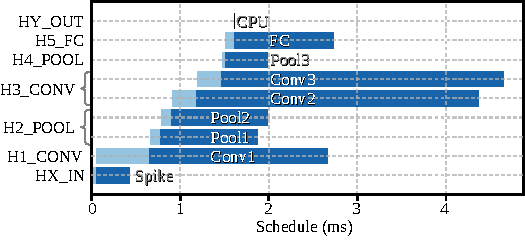
\includegraphics[width=0.5\columnwidth]{./chapters/sbs_accelerator/figures/latency_pu_fp.pdf}
	\caption{Performance of processing units with standard floating-point (IEEE 754) computation.}
	\label{fig:latency_pu_fp}
\end{figure*}

In the computation schedule, the following terms are defined as follows: $t_s(n)$ as the start time for the processing of the neural network layer (as a compute node) $n\in L$ where $L$ represents the set of layers; $t_{CPU}(n)$ as the \gls{cpu} preprocessing time; $t_{PU}(n)$ as the \gls{pu} latency; and $t_f(n)$ as the finish time. For data preparation, $t_{CPU}(n)$ is the duration in which the \gls{cpu} writes a DRAM buffer with $\vec{h}_\mu$ (vector of neuron latent variables) of the current processing layer and $S_t$ (input spike matrix) from its preceding layer. This buffer is streamed to the \gls{pu} via \gls{dma}.

The total execution time of the \gls{cpu} is defined by \Equ{eq:time_cpu}. In a cyclic spiking inference, the execution time of the network computation is the longest path among the processing units including the \gls{cpu}. This is denoted as the latency of an spike cycle and it is defined by \Equ{eq:time_spike}. The total execution time of the network computation is the last finish time ($t_f$) in the schedule defined by \Equ{eq:time_finish}.

\begin{figure*}[b!]
	\centering
	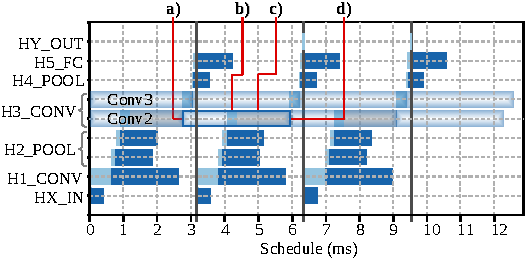
\includegraphics[width=0.5\columnwidth]{./chapters/sbs_accelerator/figures/latency_fp_cycle.pdf}
	\caption{Performance bottleneck of cyclic computation on processing units with standard floating-point (IEEE 754) arithmetic, (a) exhibits the starting of $t_{PU}$ of \emph{Conv2} on a previous computation cycle, (b) presents $t_{CPU}$ of \emph{Conv2} on the current computation cycle, (c) shows the CPU waiting time (in gray color) for \emph{Conv2} as a busy resource (awaiting for \emph{Conv2} interruption), and (d) illustrates the $t_{f}$ from the previous computation cycle, the starting of $t_{PU}$ on the current computation cycle (\emph{Conv2} interruption on completion, and start current computation cycle).}
	\label{fig:latency_pu_fp_cycle}
\end{figure*}

\begin{eqnarray} \label{eq:time_cpu}
T_{CPU} = \sum_{n\in L} t_{CPU}(n)
\end{eqnarray}

\begin{eqnarray} \label{eq:time_pu}
T_{PU} = \max_{n\in L}(t_{PU}(n))
\end{eqnarray}

\begin{eqnarray} \label{eq:time_spike}
T_{SC} =
\begin{cases}
T_{PU}, & \text{if}\ T_{CPU}\le T_{PU} \\
T_{CPU}, & \text{otherwise}
\end{cases}
\end{eqnarray}

\begin{eqnarray} \label{eq:time_finish}
T_{f} = \max_{n\in L}(t_{f}(n))
\end{eqnarray}

Using standard floating-point requires a high computational cost. As the largest layer, the computational workload of \emph{H3\_CONV} is evenly partitioned among two \glspl{pu}: \emph{Conv2} and \emph{Conv3}. However, in the cyclic schedule, \emph{Conv2} causes the performance bottleneck as shown in \Fig{fig:latency_pu_fp_cycle}. In this case, the \gls{cpu} awaits for \emph{Conv2} to finish the computation of the previous cycle in order to start the current computation cycle. In contrast, as the smallest layer, the computational workload of \emph{HY\_OUT} is fully processed by the \gls{cpu}. \Tab{tab:latency_fp} and \Fig{fig:latency_pu_fp} show \unit[4]{$\mu$s} as the processing latency of \emph{HY\_OUT}. This latency is negligible compared to the overall performance assessment. Accelerating \emph{HY\_OUT} would yield a negligible gain. Moreover, assigning a dedicated hardware \gls{pu} to \emph{HY\_OUT} would add unprofitable data transfer and hardware interruption handling overheads.

Applying \Equ{eq:time_spike}, it is obtained a latency of \unit[3.18]{ms} per spike cycle. This deployment achieves an accuracy of $98.98\%$ correct classification on the $10,000$ image test set with $1000$ spikes.

The post-implementation resource utilization and power dissipation are shown in \Tab{tab:resource_fp}. Each \emph{Conv} \gls{pu} instantiates an on-chip stationary weight matrix of $52,000$ entries, wish is sufficient to store $W\in\mathbb{R}^{5\times 5\times 2\times 32}$ and $W\in\mathbb{R}^{5\times 5\times 32\times 64}$ for \emph{H1\_CONV} and \emph{H3\_CONV}, respectively. In order to reduce BRAM utilization, we use a custom floating-point representation composed of 4-bit exponent and 4-bit mantissa (bit sign is omitted). Each 8-bit entry is promoted to its standard floating-point representation for the dot-product computation. The method to find the appropriate bit-width parameters for custom floating-point representation is presented in Section~\ref{sec:parameters}.

\begin{table}[!h]\centering
	\caption{Resource utilization and power dissipation of processing units with standard floating-point (IEEE 754) computation.}\label{tab:resource_fp}
	\scriptsize
	\begin{tabular}{lrrrrrrr}\toprule
		\textbf{PU} & &\textbf{LUT} &\textbf{FF} &\textbf{DSP} &\textbf{BRAM 18K} &\textbf{Power (mW)} \\\midrule
		Spike & &2,640 &4,903 &2 &2 &38 \\
		Conv & &2,765 &4,366 &19 &37 &89 \\
		Pool & &2,273 &3,762 &5 &3 &59 \\
		FC & &2,649 &4,189 &8 &9 &66 \\
		\bottomrule
	\end{tabular}
\end{table}

%\begin{figure}[!h]
%	\centering
%	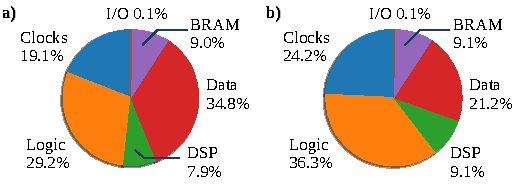
\includegraphics[width=1\columnwidth]{../figures/power_dissipation_breakdown_float-32.pdf}
%	\caption{Power dissipation breakdown of processing units with standard floating-point (IEEE 754), (a) \emph{Conv}, and (b) \emph{FC}.}
%	\label{fig:power_dissipation_breakdown_float_32}
%\end{figure}

The implementation of dot-product with standard floating-point arithmetic (IEEE 754) utilizes proprietary Xilinx multiplier and adder floating-point operator cores. Vivado \gls{hls} implements floating-point arithmetic operations by mapping them onto Xilinx LogiCORE IP cores, these floating-point operator cores are instantiated in the resultant \gls{rtl}\cite{hrica2012floating}. In this case, the implementation of the dot-product with the standard floating-point computation reuses the multiplier and adder cores already instantiated and used in other computation sections of {\emph{Conv}} and {\emph{FC}} processing units. The post-implementation resource utilization and power dissipation of the floating-point operator cores are shown in {\Tab{tab:LogiCORE}}.

\begin{table}[!h]\centering
	\caption{Resource utilization and power dissipation of multiplier and adder floating-point (IEEE 754) operator cores.}\label{tab:LogiCORE}
	\scriptsize
	\begin{tabular}{lrrrrrr}\toprule
		\textbf{Core operation} &\textbf{DSP} &\textbf{FF} &\textbf{LUT} &\textbf{Latency (clk)} &\textbf{Power (mW)} \\\midrule
		Multiplier &3 &151 &325 &4 &7 \\
		Adder &2 &324 &424 &8 &6 \\
		\bottomrule
	\end{tabular}
\end{table}

\subsubsection{Benchmark on Noise Tolerance Plot}
The purpose of the proposed noise tolerance plot is to serve as an intuitive visual model used to provide insights into accuracy degradation under approximate processing effects. This plot reveals inherent error resilience, and hence, approximation resilience. As an application-specific quality metric, this plot offers an effective method to estimate the overall quality degradation of the \gls{sbs} network under different approximate processing effects, since both approximations and noise have qualitatively the same effect~\cite{venkataramani2015approximate}.

In order to experimentally obtain the noise tolerance plot, the inference accuracy of the neural network with increasing number of spikes is measured. The measurements are retaken with uniformly distributed noise applied on the input. The levels of the noise amplitude are gradually ascended until accuracy degradation is detected. \Fig{fig:accuracy_vs_noise_pu_fp} demonstrates this method using 100 input samples.

As benchmark, the tolerance plot in \Fig{fig:accuracy_vs_noise_pu_fp} revels accuracy degradation having $50\%$ noise and convergence with $400$ spikes. In this case, the given \gls{sbs} network with precise processing demonstrates its inherent error resilience, hence, the resilience for approximate processing.


\begin{figure*}[b!]
	\centering
	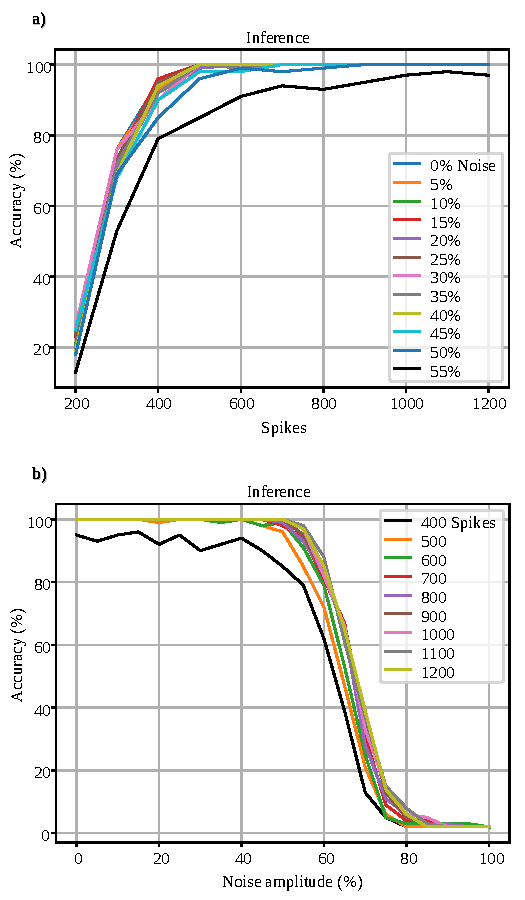
\includegraphics[width=0.5\columnwidth]{./chapters/sbs_accelerator/figures/accuracy_vs_noise_pu_fp.pdf}
	\caption{Noise tolerance on hardware PU with standard floating-point (IEEE 754) computation (benchmark/reference), (a) exhibits accuracy degradation applying $50\%$ of noise amplitude, and (b) illustrates convergence of inference with $400$ spikes.}
	\label{fig:accuracy_vs_noise_pu_fp}
\end{figure*}

\subsection{Design Exploration with Hybrid Custom Floating-Point and Logarithmic Computation}

In this section, it is presented a design exploration to evaluate the proposed approach for \gls{sbs} neural network inference using hybrid custom floating-point and logarithmic approximation. First, the synaptic weight matrix of each layer is examined in order to determine the minimum requirements for numeric representation and memory storage. Second, the proposed dot-product architecture is implemented using the minimal floating-point and logarithmic representation as design parameters. Finally, it is presented an evaluation of the overall performance, inference accuracy, resource utilization, and power dissipation.

\subsubsection{Parameters for Numeric Representation of Synaptic Weight Matrix}
\label{sec:parameters}

	The parameters for numerical representation of the synaptic weight matrices is obtained from their $\log_2$-histograms presented in {\Fig{fig:log2histogram}}. These histograms show the distribution of synaptic weight values in each matrix. The histograms show that the minimum integer exponent value is $-13$. Hence, applying {\Equ{eq:exp_max}} and {\Equ{eq:bits_exp}} to the given \gls{sbs} network, results $E_{\min}=-13$ and $N_E=4$, respectively. Therefore, 4-bits are used for the absolute binary representation of the exponents.


For quality configurability, the mantissa bit-width is a knob parameter that is tuned by the designer. This procedure leverages the builtin error-tolerance of neural networks and performs a trade-off between resource utilization and \gls{qor}. In the following subsection, a case study is presented with 1-bit mantissa. This corresponds to the custom floating-point approximation.

\begin{figure*}[b!]
	\centering
	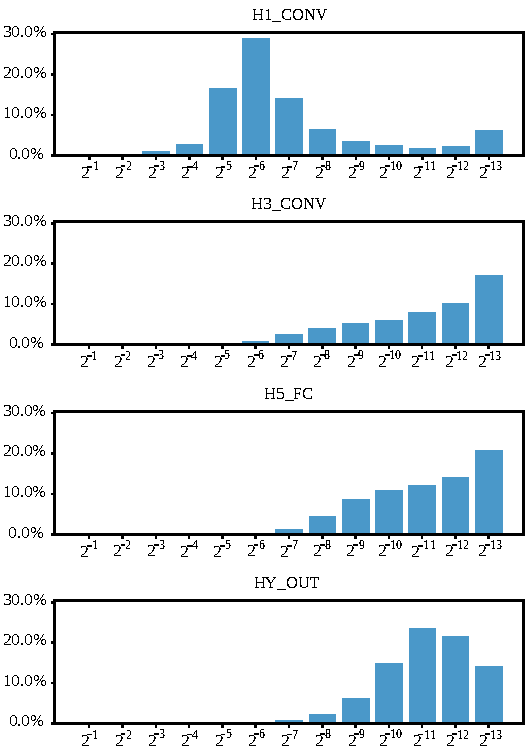
\includegraphics[width=0.5\columnwidth]{./chapters/sbs_accelerator/figures/log2_histogram.pdf}
	\caption{$\log_2$-histogram of each synaptic weight matrix showing the percentage of matrix elements with given integer exponent.}\label{fig:log2histogram}
\end{figure*}

\subsubsection{Design Exploration for Dot-product with Hybrid Custom Floating-Point Computation}
For this design exploration, a custom floating-point representation is composed of 4-bit exponent and 1-bit mantissa. This format is used for the synaptic weight vector on the proposed dot-product architecture. Each \emph{Conv} \gls{pu} instantiates an on-chip stationary weight matrix for $52,000$ entries of 5-bit. The available memory size is large enough to store $W\in\mathbb{R}^{5\times 5\times 2\times 32}$ and $W\in\mathbb{R}^{5\times 5\times 32\times 64}$ for \emph{H1\_CONV} and \emph{H3\_CONV}, respectively. The same dot-product architecture is implemented in the processing unit of the fully connected layer (\emph{FC}). However, due to lack of BRAM resources, this \gls{pu} can not instantiate on-chip stationary synaptic weight matrix. Instead, \emph{FC} receives the $\vec{W}(s_t)$ (weight vectors) during operation as well as $\vec{h}_\mu$ and $S_t$. The hardware mapping and the computation schedule of this implementation are displayed in \Tab{tab:latency_cfp} and \Fig{fig:latency_pu_cfp_cycle}.

As shown in the computation schedule in \Tab{tab:latency_cfp} and \Fig{fig:latency_pu_cfp_cycle}, this implementation presents a maximum hardware \gls{pu} latency of \unit[1.30]{ms} according to \Equ{eq:time_pu}, and \gls{cpu} latency of \unit[1.67]{ms}. Therefore, applying \Equ{eq:time_spike}, the total latency is \unit[1.67]{ms} per spike cycle as shown in \Fig{fig:latency_pu_cfp_cycle}. In this case, the cyclic bottleneck in each \gls{sbs} spike is in the \gls{cpu} performance.

This configuration achieves an accuracy of $98.97\%$ correct classification on the $10,000$ image test set with $1000$ spikes. This indicates an accuracy degradation of $0.33\%$. To monitoring output quality, the noise tolerance plot in \Fig{fig:accuracy_vs_noise_pu_cfp} revels accuracy degradation for noise higher than $50\%$ on the input images, and convergence of inference with $400$ spikes. Thus, the particular \gls{sbs} network implementation under approximate processing effects demonstrates a minimal impact on the overall accuracy. This reveals an inherent error resilience, and hence, remaining approximation budget.

The post-implementation resource utilization and power dissipation of this design are shown in \Tab{tab:resource_cfp}.

\begin{table}[h!]\centering
	\caption{Resource utilization and power dissipation of processing units with hybrid custom floating-point approximation.}\label{tab:resource_cfp}
	\scriptsize
	\begin{tabular}{lrrrrrrr}\toprule
		\textbf{PU} & &\textbf{LUT} &\textbf{FF} &\textbf{DSP} &\textbf{BRAM 18K} &\textbf{Power (mW)} \\\midrule
		Conv & &3,139 &4,850 &19 &25 &82 \\
		FC & &3,265 &5,188 &8 &9 &66 \\
		\bottomrule
	\end{tabular}
\end{table}


\begin{table}[t!]\centering
	\caption{Performance of hardware processing units with hybrid custom floating-point approximation.}\label{tab:latency_cfp}
	\scriptsize
	\begin{tabular}{llrrrrrr}\toprule
		\multicolumn{2}{c}{\textbf{Hardware mapping}} & &\multicolumn{4}{c}{\textbf{Computation schedule (ms)}} \\\cmidrule{1-2}\cmidrule{4-7}
		\textbf{Layer} &\textbf{PU} & &$t_s$ &$t_{CPU}$ &$t_{PU}$ &$t_f$ \\\midrule
		HX\_IN &Spike & &0 &0.055 &0.307 &0.362 \\
		H1\_CONV &Conv1 & &0.057 &0.654 &1.309 &2.020 \\
		\multirow{2}{*}{H2\_POOL} &Pool1 & &0.713 &0.131 &1.098 &1.942 \\
		&Pool2 & &0.845 &0.125 &1.098 &2.068 \\
		\multirow{2}{*}{H3\_CONV} &Conv2 & &0.972 &0.285 &1.199 &2.456 \\
		&Conv3 & &1.258 &0.279 &1.184 &2.721 \\
		H4\_POOL &Pool3 & &1.538 &0.037 &0.484 &2.059 \\
		H5\_FC &FC & &1.577 &0.091 &0.438 &2.106 \\
		HY\_OUT &CPU & &1.669 &0.004 &0 &1.673 \\
		\bottomrule
	\end{tabular}
\end{table}

\begin{figure*}[b!]
	\centering
	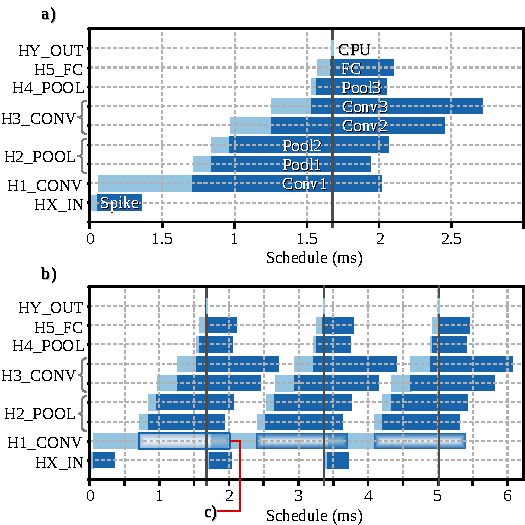
\includegraphics[width=0.5\columnwidth]{./chapters/sbs_accelerator/figures/latency_cfp_cycle.pdf}
	\caption{Performance on processing units with hybrid custom floating-point approximation, (a) exhibits computation schedule, (b) presents cyclic computation schedule, and (c) shows the performance of \emph{Conv2} from a previous computation cycle during the preprocessing of \emph{H1\_CONV} on the current computation cycle without bottleneck.}
	\label{fig:latency_pu_cfp_cycle}
\end{figure*}

\begin{figure*}[b!]
	\centering
	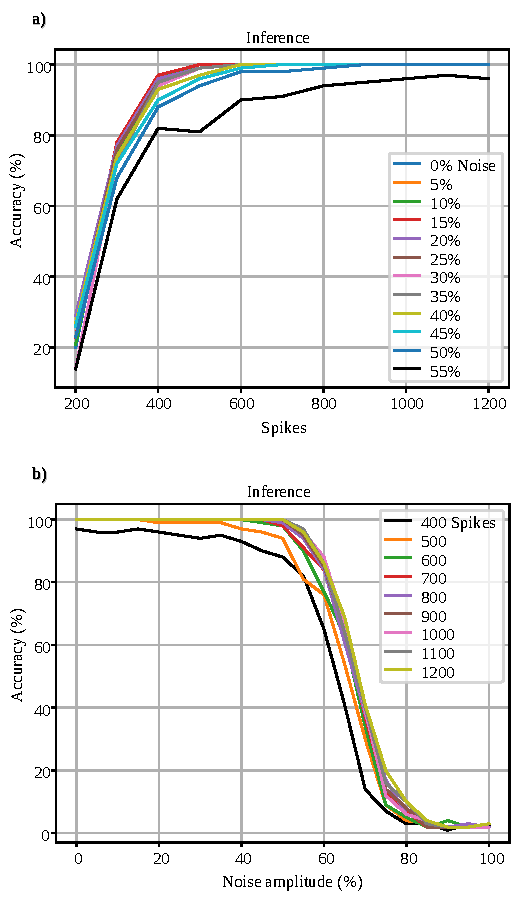
\includegraphics[width=0.5\columnwidth]{./chapters/sbs_accelerator/figures/accuracy_vs_noise_pu_cfp(4-bit-exponent_1-bit-mantissa).pdf}
	\caption{Noise tolerance on hardware PU with custom floating-point approximation, (a) exhibits accuracy degradation applying $50\%$ of noise amplitude, and (b) illustrates convergence of inference with $400$ spikes.}
	\label{fig:accuracy_vs_noise_pu_cfp}
\end{figure*}

\subsubsection{Design Exploration for Dot-Product whit Hybrid Logarithmic Computation}
For this design, 4-bit integer exponent are used for logarithmic representation of the synaptic weight matrix. Each \emph{Conv} processing unit implements the proposed dot-product architecture including an on-chip stationary weight matrix for $52,000$ entries of 4-bit integer each one to store $W\in\mathbb{N}^{5\times 5\times 2\times 32}$ and $W\in\mathbb{N}^{5\times 5\times 32\times 64}$ for \emph{H1\_CONV} and \emph{H3\_CONV}, respectively. The same dot-product architecture is implemented in the \emph{FC} processing unit without stationary synaptic weight matrix. The hardware assignment and the computation schedule of this implementation are displayed in \Tab{tab:latency_log} and \Fig{fig:latency_pu_log_cycle}.

As shown in the computation schedule in \Tab{tab:latency_log} and \Fig{fig:latency_pu_log_cycle}, this implementation presents a maximum hardware \gls{pu} latency of \unit[1.27]{ms} (according to \Equ{eq:time_pu}), and \gls{cpu} latency of \unit[1.67]{ms}. Therefore, applying \Equ{eq:time_spike}, gives \unit[1.67]{ms} as latency per spike cycle as shown in \Fig{fig:latency_pu_log_cycle}. In this case, the cyclic bottleneck is in the \gls{cpu} performance.

This quality configuration achieves an accuracy of $98.84\%$ correct classification on the $10,000$ image test set with $1000$ spikes. This indicates an accuracy degradation of $0.46\%$. To monitor output quality, the noise tolerance plot in \Fig{fig:accuracy_vs_noise_pu_log} revels accuracy degradation having $40\%$ noise on the input images, and convergence of inference with $600$ spikes. The particular \gls{sbs} network implementation under approximate processing demonstrates a minor impact on the overall accuracy. As the most efficient setup and yet the worst-case quality configuration, this exhibits remaining budget for further approximate processing approaches.

The post-implementation resource utilization and power dissipation are shown in \Tab{tab:resource_log}.

\begin{table}[t!]\centering
	\caption{Performance of hardware processing units with hybrid logarithmic approximation.}\label{tab:latency_log}
	\scriptsize
	\begin{tabular}{llrrrrrr}\toprule
		\multicolumn{2}{c}{\textbf{Hardware mapping}} & &\multicolumn{4}{c}{\textbf{Computation schedule (ms)}} \\\cmidrule{1-2}\cmidrule{4-7}
		\textbf{Layer} &\textbf{PU} & &$t_s$ &$t_{CPU}$ &$t_{PU}$ &$t_f$ \\\midrule
		HX\_IN &Spike & &0 &0.055 &0.264 &0.319 \\
		H1\_CONV &Conv1 & &0.057 &0.655 &1.271 &1.983 \\
		\multirow{2}{*}{H2\_POOL} &Pool1 & &0.714 &0.130 &1.074 &1.918 \\
		&Pool2 & &0.845 &0.126 &1.106 &2.077 \\
		\multirow{2}{*}{H3\_CONV} &Conv2 & &0.973 &0.285 &1.179 &2.437 \\
		&Conv3 & &1.258 &0.278 &1.176 &2.712 \\
		H4\_POOL &Pool3 & &1.538 &0.037 &0.488 &2.063 \\
		H5\_FC &FC & &1.577 &0.091 &0.388 &2.056 \\
		HY\_OUT &CPU & &1.669 &0.004 &0 &1.673 \\
		\bottomrule
	\end{tabular}
\end{table}

\begin{figure*}[b!]
	\centering
	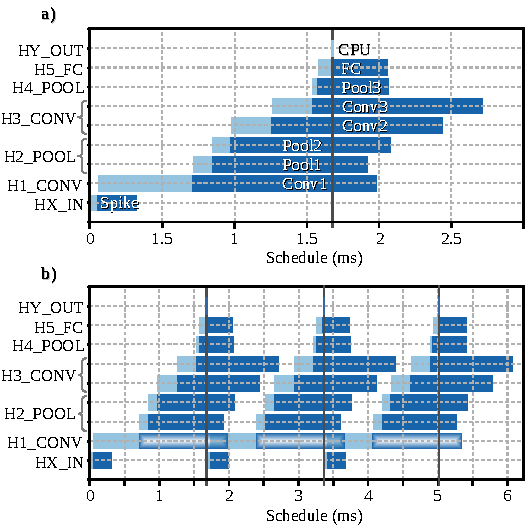
\includegraphics[width=0.5\columnwidth]{./chapters/sbs_accelerator/figures/latency_log_cycle.pdf}
	\caption{Performance of processing units with hybrid logarithmic approximation, (a) exhibits computation schedule, and (b) illustrates cyclic computation schedule.}
	\label{fig:latency_pu_log_cycle}
\end{figure*}

\begin{table}[!h]\centering
	\caption{Resource utilization and power dissipation of processing units with hybrid logarithmic approximation.}\label{tab:resource_log}
	\scriptsize
\begin{tabular}{lrrrrrrr}\toprule
	\textbf{PU} & &\textbf{LUT} &\textbf{FF} &\textbf{DSP} &\textbf{BRAM 18K} &\textbf{Power (mW)} \\\midrule
	Conv & &3,086 &4,804 &19 &21 &78 \\
	FC & &3,046 &4,873 &8 &8 &66 \\
	\bottomrule
\end{tabular}
\end{table}

%\begin{figure}[!h]
%	\centering
%	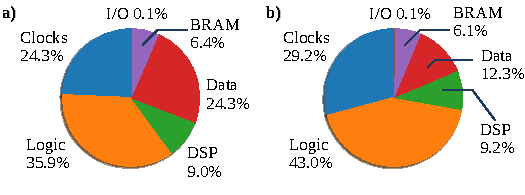
\includegraphics[width=1\columnwidth]{../figures/power_dissipation_breakdown_log-4.pdf}
%	\caption{Power dissipation breakdown of processing units with hybrid logarithmic approximation, (a) \emph{Conv}, and (b) \emph{FC}.}
%	\label{fig:power_dissipation_breakdown_log_4}
%\end{figure}



\begin{figure*}[b!]
	\centering
	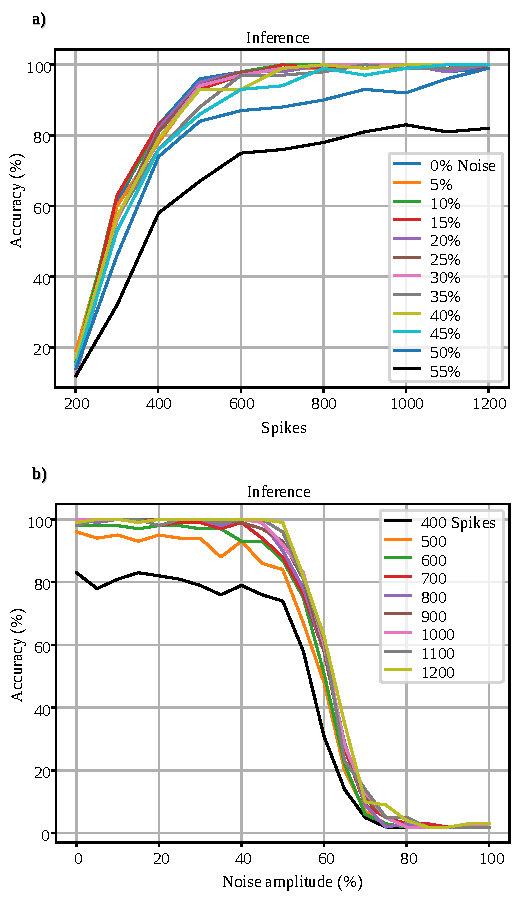
\includegraphics[width=0.5\columnwidth]{./chapters/sbs_accelerator/figures/accuracy_vs_noise_pu_log.pdf}
	\caption{Noise tolerance on hardware PU with hybrid logarithmic approximation, (a) exhibits accuracy degradation applying $40\%$ of noise amplitude, (b) illustrates convergence of inference with $600$ spikes.}
	\label{fig:accuracy_vs_noise_pu_log}
\end{figure*}


\subsection{Results and Discussion}
As benchmark, the \gls{sbs} network inference on embedded \gls{cpu} using standard 32-bit floating-point achieves an accuracy of $99.3\%$ with a latency of $T_{SC} = 34.28 ms$. As a second reference point, the network simulation on hardware processing units with standard floating-point achieves an accuracy of $98.98\%$ with a latency $T_{SC}=3.18 ms$. As result, this design get $10.7\times$ latency enhancement and an accuracy degradation of $0.32\%$. The tolerance plot in \Fig{fig:accuracy_vs_noise_pu_fp} reveals accuracy degradation having $50\%$ noise on the input images, and convergence of inference with $400$ spikes. In this case, the \gls{sbs} network deployment with precise computing proves extraordinary inherent error resilience, and hence, this represents a great potential for approximate processing.

As a demonstration of the proposed dot-product architecture, the \gls{sbs} network inference on hardware \glspl{pu} with synaptic representation using 5-bit custom floating-point (4-bit exponent, 1-bit mantissa) and 4-bit logarithmic (4-bit exponent) achieve $20.5\times$ latency enhancement and accuracy of $98.97\%$ and $98.84\%$, respectively. This results in accuracy degradation of $0.33\%$ and $0.46\%$, respectively. To monitor output quality, the noise tolerance plot in \Fig{fig:accuracy_vs_noise_pu_cfp} and \Fig{fig:accuracy_vs_noise_pu_log} reveal accuracy degradation when having $50\%$ and $40\%$ noise on the input images, and convergence of inference with $400$ and $600$ spikes, respectively. Therefore, the design exploration under the proposed approximate computing approach indicates sufficient inherent error resilience for further or more aggressive approximation approaches.

Regarding resource utilization and power dissipation with the proposed approach, \emph{Conv} processing units have a $43.24\%$ reduction of BRAM, and $12.35\%$ of improvement in energy efficiency over the standard floating-point implementation. However, the proposed approach does not reuse the available floating-point operator cores instantiated from other computational sections (see {\Tab{tab:LogiCORE}}). Therefore, the logic required for the dot-product must be implemented, which is reflected as additional utilization of \gls{lut} and \gls{ff} resources. The experimental results of the design exploration are summarized in \Tab{tab:results}. The platform implementations are summarized in \Tab{tab:platform_comparison}, and their power dissipation breakdowns are presented in \Fig{fig:platform_power_dissipation_breakdown}.

\begin{table*}[!t]
	\begin{threeparttable}
		\centering
		\caption{Experimental results.}\label{tab:results}
		\scriptsize
\begin{tabular}{lrrrrrrrrrrrr}\toprule
	\multirow{2}{*}{\textbf{Dot-product}} &\multirow{2}{*}{\textbf{PU}} &\multicolumn{4}{c}{\textbf{Post-implementation resource utilization}} &\multirow{2}{*}{\textbf{Power (mW)}} &\multicolumn{2}{c}{\textbf{Latency}} & &\multicolumn{2}{c}{\textbf{Accuracy (\%)\tnote{e}}} \\\cmidrule{3-6}\cmidrule{8-9}\cmidrule{11-12}
			& &\textbf{LUT} &\textbf{FF} &\textbf{DSP} &\textbf{BRAM 18K} & &(ms)&\textbf{Gain\tnote{d}} & &\textbf{Noise 0\%} &\textbf{50\%} \\\midrule
				\multirow{2}{*}{Standard \gls{fp}\tnote{a}} &Conv &2,765 &4,366 &19 &37 &89 &\multirow{2}{*}{3.183} &\multirow{2}{*}{10.77x} & &\multirow{2}{*}{98.98} &\multirow{2}{*}{98.63} \\
				&FC &2,649 &4,189 &8 &9 &66 & & & & & \\
				& & & & & & & & & & & \\
				\multirow{2}{*}{Hybrid custom \gls{fp}\tnote{b}} &Conv &3,139 &4,850 &19 &25 &82 &\multirow{2}{*}{1.673} &\multirow{2}{*}{20.49x} & &\multirow{2}{*}{98.97} &\multirow{2}{*}{98.47} \\
				&FC &3,265 &5,188 &8 &9 &66 & & & & & \\
				& & & & & & & & & & & \\
				\multirow{2}{*}{Hybrid log\tnote{c}} &Conv &3,086 &4,804 &19 &21 &78 &\multirow{2}{*}{1.673} &\multirow{2}{*}{20.49x} & &\multirow{2}{*}{98.84} &\multirow{2}{*}{95.22} \\
				&FC &3,046 &4,873 &8 &8 &66 & & & & & \\
				\bottomrule
			\end{tabular}
		\begin{tablenotes}
			\scriptsize
			\item[a] Reference with standard floating-point arithmetic (IEEE 754).
			\item[b] Synaptic weight with number representation composed of 4-bit exponent and 1-bit mantissa.
			\item[c] Synaptic weight with number representation composed of 4-bit exponent.
			\item[d] Acceleration with respect to the computation on embedded CPU (ARM Cortex-A9 at 666 MHz) with latency $T_{SC} = 34.28 ms$.
			\item[e] Accuracy on 10,000 image test set with 1000 spikes.
		\end{tablenotes}
	\end{threeparttable}
\end{table*}


\begin{table*}[!t]
	\begin{threeparttable}
		\centering
		\caption{Platform implementations.}\label{tab:platform_comparison}
		\scriptsize
		\begin{tabular}{lrrrrrrrrrr}\toprule
			\multirow{2}{*}{\textbf{Platform implementation}} &\multicolumn{4}{c}{\textbf{Post-implementation resource utilization}} &\multirow{2}{*}{\textbf{Power (W)}} &\multirow{2}{*}{\textbf{Clk (MHz)}} &\multicolumn{2}{c}{\textbf{Latency}} &\multirow{2}{*}{\textbf{Accu (\%)\tnote{f}}} \\\cmidrule{2-5}\cmidrule{8-9}
			&\textbf{LUT} &\textbf{FF} &\textbf{DSP} &\textbf{BRAM 18K} & & &\textbf{(ms)} &\textbf{Gain\tnote{e}} & \\\midrule
			\cite{nevarez2020accelerator}\tnote{a} &42,740 &57,118 &49 &92 &2.519 &250 &4.65 &7.4x &99.02 \\
			This work (standard \gls{fp})\tnote{b} &39,514 &56,036 &82 &180 &2.420 &200 &3.18 &10.7x &98.98 \\
			This work (hybrid custom \gls{fp})\tnote{c} &42,021 &58,759 &82 &156 &2.369 &200 &1.67 &20.5x &98.97 \\
			This work (hybrid log)\tnote{d} &41,060 &57,862 &82 &148 &2.324 &200 &1.67 &20.5x &98.84 \\
			\bottomrule
		\end{tabular}
		\begin{tablenotes}
			\scriptsize
			\item[a] Reference architecture with homogeneous AUs using standard floating-point arithmetic (IEEE 754).
			\item[b] Reference architecture with specialized heterogeneous PUs using standard floating-point arithmetic (IEEE 754).
			\item[c] Proposed architecture with specialized heterogeneous PUs using synaptic weight with number representation composed of 4-bit exponent and 1-bit mantissa.
			\item[d] Proposed architecture with specialized heterogeneous PUs using synaptic weight with number representation composed of 4-bit exponent.
			\item[e] Acceleration with respect to the computation on embedded CPU (ARM Cortex-A9 at 666 MHz) with latency $T_{SC} = 34.28 ms$.
			\item[f] Accuracy on 10,000 image test set with 1000 spikes.
		\end{tablenotes}
	\end{threeparttable}
\end{table*}

\begin{figure*}[b!]
	\centering
	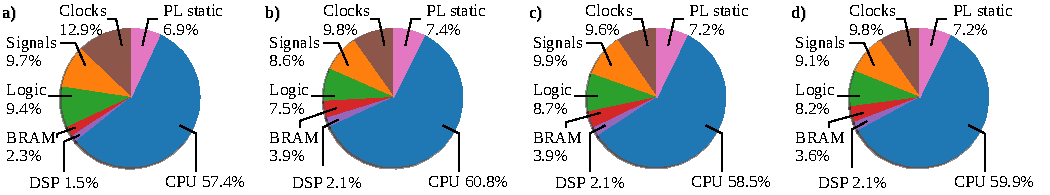
\includegraphics[width=\columnwidth]{./chapters/sbs_accelerator/figures/platform_power_dissipation_breakdown.pdf}
	\caption{Power dissipation breakdown of platform implementations, (a) \cite{nevarez2020accelerator} architecture with homogeneous AUs using standard floating-point arithmetic (IEEE 754), (b) reference architecture with specialized heterogeneous PUs using standard floating-point arithmetic (IEEE 754), (c) proposed architecture with hybrid custom floating-point approximation, and (d) proposed architecture with hybrid logarithmic approximation.}
	\label{fig:platform_power_dissipation_breakdown}
\end{figure*}
\section{Conclusions}
\label{sec:conclusions}
This chapter presents an accelerator for \gls{sbs} neural networks with a dot-product functional unit based on approximate computing that combines the advantages of custom floating-point and logarithmic representations. This approach reduces computational latency, memory footprint, and power dissipation while preserving accuracy. For output quality monitoring, noise tolerance plots are proposed as an intuitive visual measure to provide insights into the accuracy degradation of \gls{sbs} networks under different approximate processing effects. This plot revels inherent error resilience, hence, the possibilities for approximate processing.


The proposed approach is demonstrated with a design exploration flow on a Xilinx Zynq-7020 with a deployment of \gls{sbs} network for MNIST classification task. This implementation achieves up to $20.5\times$ latency enhancement, $8\times$ weight memory footprint reduction, and $12.35\%$ of energy efficiency improvement over the standard floating-point hardware implementation, this deployment incurs in less than $0.5\%$ of accuracy degradation. Furthermore, with noise amplitude of $50\%$ added on the input images, the \gls{sbs} network presents an accuracy degradation of less than $5\%$. To monitor the inference quality, the resulting noise tolerance plots demonstrate a sufficient \gls{qor} for minimal impact on the overall accuracy of the neural network under the effects of this approximation technique. These results suggest available room for further or more aggressive approximate processing approaches.


In summary, based on the relaxed need for fully accurate or deterministic computation of neural networks, approximate computing techniques allow substantial enhancement in processing efficiency with moderated accuracy degradation.

\chapter{Accelerating Convolutional Neural Networks: Hybrid 6-bit Floating-Point Computation}\label{chap.cnn}
\minitoc
\section{Abstract}
\begin{quote}
	This chapter introduces a novel hardware design methodology tailored for low-power \gls{cnn} inference in sensor analytics applications. Central to this approach is the \gls{hf6} quantization scheme, which utilizes a hybrid number representation that blends standard \gls{fp} with a 6-bit \gls{fp} format. This unique combination facilitates a more efficient \gls{fp} \gls{mac}, transforming the typical mantissa multiplication into a simplified multiplexer-adder operation. The custom \gls{fp} \gls{mac} is integrated in a dedicated hardware accelerator designed to function as a Conv2D tensor processor. To complement the benefits of the \gls{hf6} scheme, this research introduces a \gls{qat} method which, in certain cases, offers beneficial regularization effects. The efficacy of this approach is showcased through a regression model that achieves enhanced accuracy despite the applied quantization. Prioritizing \gls{ml} portability, this design encapsulates the custom \gls{fp} representation within a standard format, which is automatically processed by the proposed tensor processor. To validate interoperability of this approach, the hardware architecture is integrated with TensorFlow Lite, demonstrating compatibility with industry-standard \gls{ml} frameworks and affirming the potential for practical deployment in various applications while maintaining compliance with established \gls{ml} infrastructure.
\end{quote}

\section{Introduction}
\label{sec:introduction}
%%% General intro
There is a growing demand for sensor analytics based on \gls{ml} algorithms. Industry 4.0 and smart city infrastructure leverage \gls{ai} solutions to increase productivity and adaptability~\cite{lom2016industry}. These solutions are powered by advances in \gls{ml}, compute engines, and big data. Therefore, enhancement of these should be considered for research, as they are the machinery of the future.

\glspl{cnn} represent the essential building blocks in 2D pattern analytics. Sensor-based applications such as mechanical fault diagnosis~\cite{li2019sensor,dong2018rolling}, structural health monitoring~\cite{nagayama2007structural}, human activity recognition~\cite{wang2019deep}, hazardous gas detection~\cite{kim2017hazardous} have been powered by \gls{cnn} models in industry and academia. \gls{cnn}-based models, as one of the main types of \gls{ann}, have been widely used in sensor analytics with automatic learning from sensor data~\cite{ince2016real, janssens2016convolutional, abdeljaber2017real, guo2016hierarchical}. In this context, \gls{cnn} models are applied for automatic feature learning, usually, from 1D time series as well as for 2D time-frequency spectrograms. \gls{cnn} models provide advantages such as local dependency, scale invariance, and noise resilience in analytics~\cite{du2014leveraging}. However, \gls{cnn} models are computationally intensive and power-hungry. This is particularly challenging for low-power embedded applications, such as in the \gls{iot} field.

For \gls{ml} inference, dedicated hardware architectures are typically used to enhance compute performance and power efficiency. In terms of computational throughput, \glspl{gpu} offer the highest performance; in terms of power efficiency, \gls{asic} and \gls{fpga} solutions are more energy efficient~\cite{nurvitadhi2017can}. As a result, numerous commercial \gls{asic} and \gls{fpga} accelerators have been proposed, targeting both \gls{hpc} for data-centers and embedded systems applications.

However, most \gls{fpga} accelerators have been implemented to target mid- to high-range \glspl{fpga} for computationally intensive \gls{cnn} models such as AlexNet, VGG-16, and ResNet-18. The main drawbacks of these implementations are power supply demands, physical dimensions, heat sink requirements, air cooling, and high price. In some cases, these implementations are not feasible for ubiquitous low-power/resource-constrained applications.

To reduce hardware there are two types of research~\cite{wu2021low}: the first one is deep compression including weight pruning, weight quantization, and compression storage~\cite{han2015deep,han2015learning}; the second type of research corresponds to a more efficient data representation, also known as custom quantization for dedicated hardware implementation. In this group, hardware implementations with customized 8-bit floating-point computation have been proposed~\cite{mei2017200mhz, wu2021low, lian2019high}. However, these architectures are inadequate for embedded applications, the target devices are high-end \glspl{fpga} and PCIe devices.

Reducing the compute hardware with more aggressive quantization such as binary~\cite{courbariaux2015binaryconnect}, ternary~\cite{lin2015neural}, and mixed precision (2-bit activations and ternary weights)~\cite{colangelo2018exploration} typically incur significant accuracy degradation for very low precisions, especially for complex problems that require precision~\cite{faraone2019addnet}.

In this chapter, it is presented the Hybrid-Float6 quantization and its dedicated hardware design. In this approach, feature maps are represented by a standard \gls{fp} number representation and trainable parameters by 6-bit \gls{fp}. To preserve accuracy, a \gls{qat} method is proposed. For \gls{ml} compatibility/portability, the 6-bit FP can be wrapped into the standard \gls{fp} number representation. It is presented a parameterized tensor processor implementing a pipelined vector dot-product with \gls{hf6}. The proposed hardware extracts the 6-bit representation automatically from the standard \gls{fp} format and performs the computation. The 6-bit \gls{fp} representation uses 4-bit exponent and 1-bit mantissa. This approach enables optimizations in \gls{mac} design by reducing the mantissa multiplication to a multiplexer-adder operation. Moreover, the intrinsic error tolerance of \gls{ann} is leveraged to further reduce the hardware design with approximation. This approach reduces latency, resource utilization, and power dissipation. The embedded hardware/software architecture is integrated with TensorFlow Lite using delegate interface to accelerate \emph{Conv2D} tensor operations. We evaluate the applicability of our approach with a \gls{cnn}-regression model and hardware design exploration for sensor analytics of \gls{shm} for anomaly localization. The embedded hardware/software framework is demonstrated on XC7Z007S, this is the smallest and most inexpensive Zynq \gls{soc} device, see \Fig{fig:workflow}. To the best of my knowledge, this is the first research addressing 6-bit floating-point quantization on \gls{cnn} models and its dedicated hardware design.

\begin{figure}[t!]
	\centering
	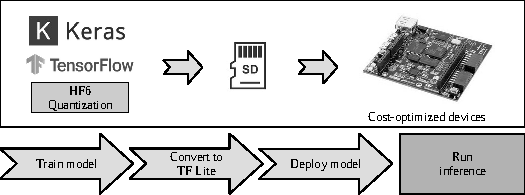
\includegraphics[width=0.5\textwidth]{./chapters/cnn_accelerator/figures/workflow.pdf}
	\caption{The workflow of our approach on embedded FPGAs.}
	\label{fig:workflow}
\end{figure}

The main contributions presented in this chapter are as follows:
\begin{enumerate}
	\item
	
	The Hybrid-Float6 quantization and its dedicated hardware design. It is proposed an optimized hardware \gls{mac} by reducing the mantissa multiplication to a multiplexer-adder operation. The intrinsic error tolerance of \gls{ann} is exploited to further reduce the hardware design with approximation. To preserve model accuracy, it is presented a quantization-aware training method, which provides regularization effects.
	
	\item A custom hardware/software co-design framework for low-power analytics on resource-constrained embedded \gls{fpga}. TensorFlow Lite micro is integrated in this framework.
	\item A customizable tensor processor as a dedicated hardware for \gls{hf6}. This design computes \emph{Conv2D} tensor operations employing a pipelined vector dot-product with parametrized on-chip memory utilization. For exploration purposes, the compute engine can be synthesized with the proposed \gls{hf6} hardware or with Xilinx LogiCORE IPs (for standard floating-point).
	\item The potential of this approach is demonstrated with a \gls{cnn}-regression model for anomaly localization in \gls{shm} based on \gls{ae}. A hardware design exploration is presented evaluating inference accuracy, compute performance, hardware resource utilization, and energy consumption.
\end{enumerate}

This work is available to the community as an open-source project at

https://github.com/YaribNevarez/tensorflow-lite-fpga-delegate.git.
%\section{Related work}
\label{sec:related_work}
In the literature we find plenty of hardware architectures for \gls{cnn} accelerators implemented in \gls{fpga}. Most of the research work implements fixed-point quantization, and very limited research focuses on \gls{fp}. Moreover, to the best of my knowledge, there is no research work related to \gls{fp} inference for low-power embedded applications.


\subsection{Hybrid Custom Floating-Point}
In \cite{lai2017deep}, Liangzhen Lai et al. proposed a mixed data representation with floating-point for weights and fixed-point for activations. This work demonstrated on SqueezeNet, AlexNet, GoogLeNet, and VGG-16 that 8-bit floating-point quantization (4-bit exponent and 3-bit mantissa) results in constant negligible accuracy degradation. Similarly, in \cite{settle2018quantizing}, Sean O. Settle et al. presented an 8-bit \gls{fp} quantization scheme, which needs an extra inference batch to compensate for quantization errors. However, \cite{lai2017deep} and \cite{settle2018quantizing} did not present a dedicated hardware architecture.

In \cite{lian2019high}, Xiaocong Lian et al. proposed a hardware accelerator with optimized block floating-point (BFP). In this design the activations and weights are represented by 16-bit and 8-bit \gls{fp} formats, respectively. This design is demonstrated on Xilinx VC709 evaluation board. This implementation achieves throughput and power efficiency of \unit[760.83]{GOP/s} and \unit[82.88]{GOP/s/W}, respectively. However, this design is not suitable for low-power resource-constrained embedded \glspl{fpga}.

\subsection{Low-Precision Floating-Point}
In \cite{mei2017200mhz}, Chunsheng Mei et al. presented a hardware accelerator for VGG16 model using half-precision \gls{fp} (16-bit). This design is demonstrated on Xilinx Virtex-7 (XC7VX690T) with PCIe interface. This implementation achieves throughput and power efficiency of \unit[202.8]{GFLOP/s} and \unit[18.72]{GFLOP/s/W}, respectively. In \cite{wu2021low}, Chen Wu et al. proposed a low-precision (8-bit) floating-point (LPFP) quantization method for \gls{fpga}-based acceleration. This design is demonstrated on Xilinx Kintex 7 and Ultrascale/Ultrascale+. This implementation achieves throughput and power efficiency of \unit[1086.8]{GOP/s} and \unit[115.4]{GOP/s/W}, respectively.

\subsection{Low-Power}
Two research papers have been reported hardware accelerators targeting XC7Z007S. This is the smallest and most inexpensive device from Zynq-7000 SoC family. In \cite{meloni2019cnn}, Paolo Meloni et al. presented a \gls{cnn} inference accelerator for compact and cost-optimized devices. This implementation uses fixed-point to process light-weight \gls{cnn} architectures with a power efficiency between \unit[2.49] to \unit[2.98]{GOPS/s/W}. In \cite{gao2020edgedrnn}, Chang Gao et al. presented EdgeDRNN, a \gls{rnn} accelerator for edge inference. This implementation adopts the \gls{snn} inspired delta network algorithm to exploit temporal sparsity in \glspl{rnn}.
\section{System Design}
\label{sec:system_design}
The system design is a hardware/software co-design framework for low-power \gls{ml} analytics. This architecture allows design exploration for dedicated hardware in embedded systems. For \gls{ml} compatibility, the proposed framework integrates TensorFlow Lite micro.

\subsection{Base embedded system architecture}
The embedded system architecture consists of a cooperative hardware-software platform. See \Fig{fig:system_architecture}. The embedded \gls{cpu} delegates low-level compute-bound tensor operations to the \glspl{tp}. The \glspl{tp} employ AXI-Lite interface for configuration and AXI-Stream interfaces via \gls{dma} for data movement from off-chip memory. Each \gls{tp} and \gls{dma} pair asserts interrupt flags once its compute job/transaction completes. Interrupt events are handled by the embedded \gls{cpu} to use the results and to start a new compute job/transaction. The hardware architecture can vary its resource utilization by customizing the \glspl{tp} prior to the hardware synthesis.
\begin{figure}[t!]
	\centering
	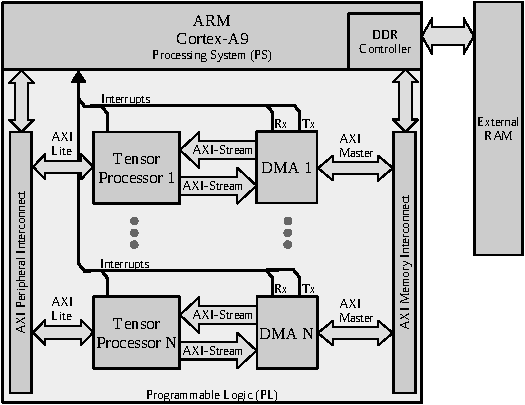
\includegraphics[width=0.5\textwidth]{./chapters/cnn_accelerator/figures/system_design.pdf}
	\caption{Base embedded system architecture.}
	\label{fig:system_architecture}
\end{figure}
\subsection{Tensor processor}
The \gls{tp} is a dedicated hardware module to compute tensor operations. This implements high performance communication with AXI-Stream, direct \gls{cpu} communication with AXI-Lite, and on-chip storage utilizing BRAM. This hardware architecture is implemented with \gls{hls}. The tensor operations are implemented based on the C++ TensorFlow Lite micro kernels. See \fig{fig:accelerator}. This research focuses on the \emph{Conv2D} tensor operation that computes 2D convolution layers.

\begin{figure}[t!]
	\centering
	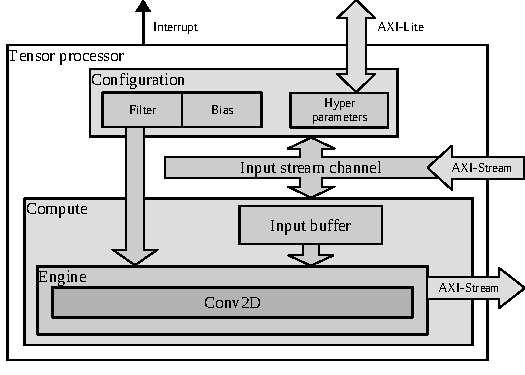
\includegraphics[width=0.5\textwidth]{./chapters/cnn_accelerator/figures/accelerator.pdf}
	\caption{High level hardware architecture of the proposed tensor processor.}
	\label{fig:accelerator}
\end{figure}
\subsubsection{Modes of operation}
The \gls{tp} has two modes of operation: \emph{configuration} and \emph{execution}.
\begin{itemize}
	\item In \emph{configuration} mode, the \gls{tp} receives the hyperparameters of the tensor operation: stride, dilation, padding, offset, activation, depth-multiplier, input shape, filter shape, bias shape, and output shape. Afterwards, in the same data stream, the \gls{tp} receives filter and bias tensors. These are locally stored in BRAM for data re-usage. The filter and bias tensors are transferred using standard \gls{fp} format wrapping the 6-bit \gls{fp} representation, which is extracted by the \gls{tp} for local on-chip storage.
	
	\item In \emph{execution} mode, the \gls{tp} executes the tensor operation according to the hyperparameters given in the configuration mode. During execution, the input and output tensors are moved via \gls{dma}.
\end{itemize}
\subsubsection{Dot-product with hybrid floating-point}
\label{sec:dot_product}
We implement the floating-point computation adopting the dot-product with hybrid custom floating-point~\cite{nevarez2021accelerating}. The hardware dot-product is illustrated in \Fig{fig:dot_product} and \Fig{fig:dot_product_loop}(a). This design instantiates a HF6 \gls{mac} with an internal accumulator register of 64-bit fixed-point with 23-bit fraction. During operation, the feature map and filter values are extracted from on-chip memory (BRAM). Both values have to be different than zero to enable the \gls{mac} operation. The result is biased by accumulating a denormalized bias value. Since the bias is stored with 6-bit \gls{fp}, its fractional part has to be aligned with the 23-bit fraction of the accumulator, see \Fig{fig:dot_product_loop}(b). The ReLu activation is applied to the accumulator and its result is normalized to convert it to IEEE 754 standard \gls{fp}, see \Fig{fig:dot_product_loop}(c).

Rather than a parallelized hardware structure, this approach is a pipelined hardware design suitable for resource-limited devices. The latency in clock cycles of this hardware module is defined by \equ{eq:dot_custom_float_latency}, where $N$ is the length for the vector dot-product. This latency equation is obtained from the general pipelined hardware latency formula: $L=\left(N-1\right)II+IL$, where $II$ is the initiation interval, and $IL$ is the iteration latency. Both $II$ and $IL$ are obtained from the \gls{hls} results. Both the exponent and mantissa bit widths of the filter and bias are set to 4-bit exponent and 1-bit mantissa (E4M1), which corresponds to float6 quantization.

\begin{eqnarray} \label{eq:dot_custom_float_latency}
L_{hf}=N+7
\end{eqnarray}

\begin{figure}[t!]
	\centering
	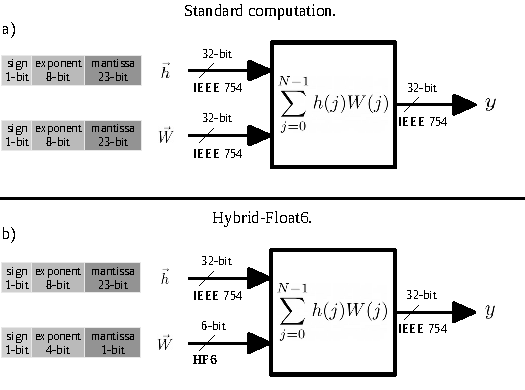
\includegraphics[width=0.5\textwidth]{./chapters/cnn_accelerator/figures/dot-product_unit.pdf}
	\caption{Dot-product hardware module with (a) standard floating-point and (b) Hybrid-Float6.}
	\label{fig:dot_product}
\end{figure}

\begin{figure}[t!]
	\centering
	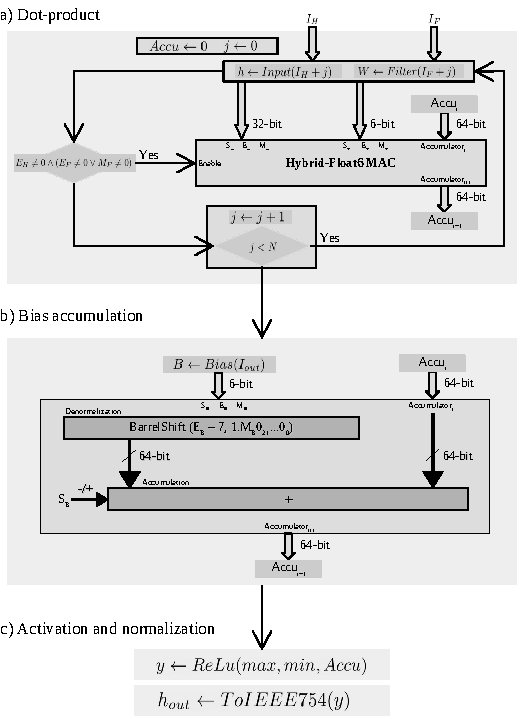
\includegraphics[width=0.5\textwidth]{./chapters/cnn_accelerator/figures/dot_product_hybrid.pdf}
	\caption{(a) Dot-product hardware module with Hybrid-Float6 MAC, (b) bias accumulation, (c) activation and normalization to IEEE754.}
	\label{fig:dot_product_loop}
\end{figure}

\subsubsection{Multiply-Accumulate}
The multiply-accumulate operation calculates the product of two numbers and adds the result to an accumulator. In \gls{fp} arithmetics, the area of a hardware multiplier scales with the bit size of the mantissas. In the case of \gls{hf6}, the 6-bit \gls{fp} representation allows a reduced hardware multiplicator for mantissas. The 1-bit mantissa enables optimized \gls{mac} implementations by reducing the mantissa multiplication to a multiplexed addition, see \fig{fig:multiplier}. This \gls{mac} produces denormalized results, which are accumulated in a fixed-point accumulator. This approach reduces latency, energy consumption, and hardware area/resource utilization.

\begin{figure}[t!]
	\centering
	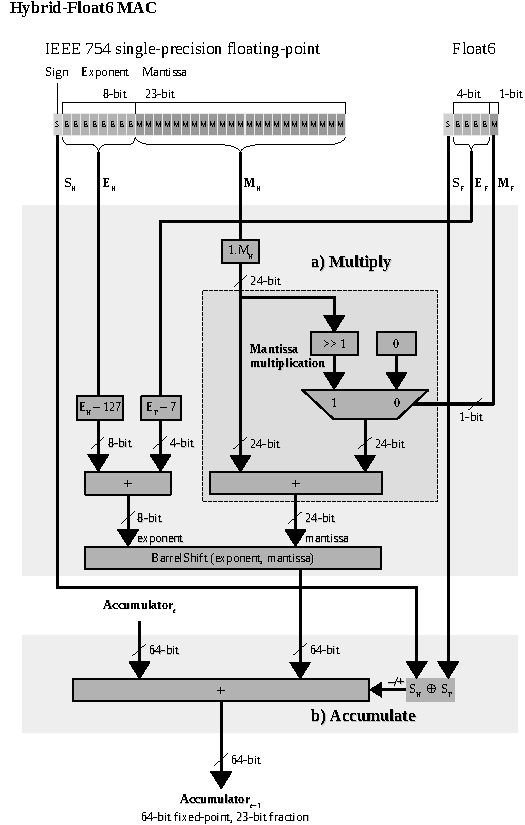
\includegraphics[width=0.5\textwidth]{./chapters/cnn_accelerator/figures/multiplier.pdf}
	\caption{Hybrid-Float6 multiply-accumulate hardware design.}
	\label{fig:multiplier}
\end{figure}

Special cases, such as Infinity and \gls{nan}, are not considered in this design for simplicity, since they are not expected for \gls{cnn} inference. For the subnormal case, the element-wise multiplication is disabled when having a zero entry and approximated when having subnormal mantissa. The feature map values are considered zero when the exponent is zero ($E_H=0$). The filter values are considered zero when both exponent and mantissa are zero ($E_F=0\land M_F=0$). See \Fig{fig:dot_product_loop}(a). In the 6-bit \gls{fp}, the 1-bit mantissa has one subnormal case, which is handled as a normalized case. This exploits the intrinsic error tolerance to reduce the hardware design.

The approximation error is defined by the difference between \Equ{eq:float} and \Equ{eq:float_subnorm} when $E=0$ and $M=2^{-1}$. The result defines the error as $e=2^{-B-1}$. Then, from \Equ{eq:float_bias} with $E_{size}=4$, gives $B=7$. Hence, $e=3.9\mathrm{e}{-3}$. This error is produced when having the subnormal case $E=0$ and $M=2^{-1}$, which corresponds to the value $\pm7.8\mathrm{e}{-3}$ deviated to $\pm1.17\mathrm{e}{-2}$. This approximation leverages the intrinsic error tolerance of \gls{cnn} to reduce hardware resource utilization and energy consumption~\cite{du2014leveraging}.


\subsubsection{On-chip memory utilization}
\label{sec:memory_utilization}
The total on-chip memory utilization on the \gls{tp} is defined by \Equ{eq:tp_memory}, where $TP_B$ and $V_{M}$ represent the tensor buffers required for \emph{Conv} operation and local registers required for the logic, respectively. \Equ{eq:tp_memory_buffer} defines the tensor buffers, where $Input_{M}$ is the \emph{input buffer}, $Filter_{M}$ is the \emph{filter buffer}, $Bias_{M}$ is the \emph{bias buffer}. These on-chip memory buffers are defined in bits. \fig{fig:accelerator_buffers} illustrates the convolution operation utilizing the on-chip memory buffers.
\begin{figure}[t!]
	\centering
	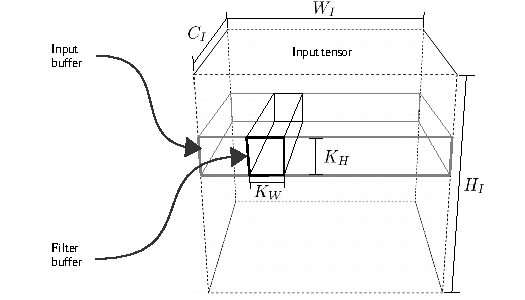
\includegraphics[width=0.5\textwidth]{./chapters/cnn_accelerator/figures/accelerator_buffers.pdf}
	\caption{Design parameters for on-chip memory buffers on the TP.}
	\label{fig:accelerator_buffers}
\end{figure}
\begin{eqnarray} \label{eq:tp_memory}
TP_{M}=TP_B+V_{M}
\end{eqnarray}
\begin{eqnarray} \label{eq:tp_memory_buffer}
TP_{B}=Input_{M}+Filter_{M}+Bias_{M}
\end{eqnarray}

The memory utilization of \emph{input buffer} is defined by \Equ{eq:input_memory}, where $K_{H}$ is the height of the convolution kernel, $W_{I}$ is the width of the input tensor (input feature maps), $C_{I}$ is the number of input channels, and $BitSize_{I}$ is the bit size representation used by the input tensor.
\begin{eqnarray} \label{eq:input_memory}
Input_{M}=K_{H}W_{I}C_{I}BitSize_{I}
\end{eqnarray}

The memory utilization of \emph{filter buffer} is defined by \Equ{eq:filter_memory}, where $K_{W}$ and $K_{H}$ are the width and height of the convolution kernel, respectively; $C_{I}$ and $C_{O}$ are the number of input and output channels, respectively; and $BitSize_{F}$ is the bit size representation used by filter values.
\begin{eqnarray} \label{eq:filter_memory}
Filter_{M}=C_{I}K_{W}K_{H}C_{O}BitSize_{F}
\end{eqnarray}

The memory utilization of \emph{bias buffer} is defined by \Equ{eq:bias_memory}, where $C_{O}$ is the number of output channels, and $BitSize_{B}$ is the bit size representation used by bias values.
\begin{eqnarray} \label{eq:bias_memory}
Bias_{M}=C_{O}BitSize_{B}
\end{eqnarray}

As a design trade-off, \Equ{eq:channel_in_memory} defines the capacity of output channels based on given design parameters. The total on-chip memory $TP_{M}$ determines the \gls{tp} storage capacity.
\begin{eqnarray} \label{eq:channel_in_memory}
C_{O}=\frac{TP_{M}-V_{M}-K_{H}W_{I}C_{I}BitSize_{I}}{C_{I}K_{W}K_{H}BitSize_{F}+BitSize_{B}}
\end{eqnarray}

The floating-point formats implemented in the \gls{tp} are defined by $BitSize_F$, $BitSize_B$ and $BitSize_I$. The HF6 defines 6-bit for $BitSize_F$ and $BitSize_B$, and 32-bit for $BitSize_I$. These are design parameters defined before hardware synthesis. This allows fine control of BRAM utilization, which is suitable for resource-limited devices.

\subsection{Training Method}
The training method consists of two separate stages: (1) training with iterative early stop and (2) quantization-aware training.
 
\subsubsection{Training with Iterative Early Stop}
To achieve better performance on \gls{cnn}-regression models, it implemented a training procedure with iterative early stop cycle. This allows to reach better local minima. This process consists of four steps:

\begin{enumerate}
	\item A model is obtained with an initial training with standard early stop monitoring.
	\item The model is iteratively re-trained with standard early stop. This process iteratively restarts the moving averages of the optimizer to search for better local minima.
	\item In case of a better local minimum, the model is saved and used as a base for subsequent search iterations, otherwise it is a discarded search.
	\item The cyclic process stops automatically with a given number of searches without a better local minimum, this is denoted as stop patience. This allows to set a maximum number of unsuccessful search trials before the stop.
\end{enumerate}

This method is described in \Algo{alg:training}.

\subsubsection{Quantization-Aware Training}
The \gls{qat} method is integrated into the training process, this operates as a callback on each mini-batch update. The quantization is applied on the trainable parameters of convolution layers. This method is implemented on the \gls{ml} framework (TensorFlow/Keras), see \Algo{alg:quantization_integration}.

The quantization method uses rounding strategy to reduce the \gls{fp} representation. This maps the full precision \gls{fp} values to the closest representable 6-bit \gls{fp} values, see \Algo{alg:quantize_training}. This method quantizes the filter and bias tensors of the convolution layers. The exponent bit size plays a more predominant influence on the model accuracy than the mantissa bit size. In \cite{lai2017deep}, Lai et al. demonstrated that 4-bit exponent and X-bit mantissa is adequate and consistent across different networks (SqueezeNet, AlexNet, GoogLeNet, VGG-16). In this research, the \gls{fp} representation with 4-bit exponent and 1-bit mantissa is investigated.

\begin{algorithm}[h!]
	\caption{Training with iterative early stop cycle.}
	\label{alg:training}
	\begin{algorithmic}
		\SetAlgoLined
		\renewcommand{\algorithmicrequire}{\textbf{input:}}
		\renewcommand{\algorithmicensure}{\textbf{output:}}
		\REQUIRE $MODEL$ as the input model.
		\REQUIRE $D_{train}$ as the training data set.
		\REQUIRE $D_{val}$ as the validation data set.
		\REQUIRE $N_{I}$ as the stop patience for iterative training cycle.
		\REQUIRE $N_{E}$ as the early stop patience (epochs) for training.
		\REQUIRE $B_{size}$ as the mini-batch size.
		\ENSURE $MODEL$ as the full-precision output model.
		\STATE $Train(MODEL, D_{train}, D_{val}, N_{E}, B_{size})$
		\STATE $mse_i \gets Evaluate(MODEL, D_{val})$ // Benchmark
		\STATE $n_I \gets 0$
		\WHILE {$n_I<N_I$}
		\STATE // Iterative early stop cycle
		\STATE $Train(MODEL, D_{train}, D_{val}, N_{E}, B_{size})$
		\STATE $mse_v \gets Evaluate(MODEL, D_{val})$
		\IF{$mse_v < mse_i$}
			\STATE $Update(MODEL)$
			\STATE $mse_i \gets mse_v$
		\ELSE
			\STATE $MODEL  \gets LoadPreviousWeights()$
			\STATE $n_I \gets n_I + 1$
		\ENDIF
		\ENDWHILE
	\end{algorithmic}
\end{algorithm}


\begin{algorithm}[h!]
	\caption{OnMiniBatchUpdate\_Callback.}
	\label{alg:quantization_integration}
	\begin{algorithmic}
		\SetAlgoLined
		\renewcommand{\algorithmicrequire}{\textbf{input:}}
		\renewcommand{\algorithmicensure}{\textbf{output:}}
		\REQUIRE $MODEL$ as the full-precision input model.
		\REQUIRE $E_{size}$ as the target exponent bits size.
		\REQUIRE $M_{size}$ as the target mantissa bits size.
		\REQUIRE $D_{train}$ as the training data set.
		\REQUIRE $D_{val}$ as the validation data set.
		\REQUIRE $N_{ep}$ as the number of epochs.
		\REQUIRE $B_{size}$ as the mini-batch size.
		\ENSURE $MODEL$ as the quantized output model.
		\STATE // Quantize
		\STATE $MODEL \gets$ \Algo{alg:quantize_training}$(MODEL,E_{size}, M_{size})$ 
		\IF {$1<epoch$}
		\STATE // Update model after first epoch
		\STATE $mse_v \gets Evaluate(MODEL, D_{val})$
		\IF{$mse_v < mse_i$}
		\STATE $Update(MODEL)$
		\STATE $mse_i \gets mse_v$
		\ENDIF
		\ENDIF
	\end{algorithmic}
\end{algorithm}

\begin{algorithm}[h!]
	\caption{Custom floating-point quantization.}
	\label{alg:quantize_training}
	\begin{algorithmic}
		\SetAlgoLined
		\renewcommand{\algorithmicrequire}{\textbf{input:}}
		\renewcommand{\algorithmicensure}{\textbf{output:}}
		\REQUIRE $MODEL$ as the CNN.
		\REQUIRE $E_{size}$ as the target exponent bit size.
		\REQUIRE $M_{size}$ as the target mantissa bits size.
		\REQUIRE $STDM_{size}$ as the IEEE 754 mantissa bit size.
		\ENSURE $MODEL$ as the quantized CNN.
		\FOR {$layer$ in $MODEL$}
		\IF {$layer$ is $Conv2D$ or $SeparableConv2D$}
		\STATE $filter, bias \gets GetWeights(layer)$
		\FOR {$x$ in $filter$ and $bias$}
			\STATE $sign \gets GetSign(x)$
			\STATE $exp \gets GetExponent(x)$
			\STATE $fullexp \gets 2^{E_{size}-1}-1$ // Get full range value
			\STATE $cman \gets GetCustomMantissa(x, M_{size})$
			\STATE $leftman \gets GetLeftoverMantissa(x, M_{size})$
			\IF {$exp <-fullexp$}
				\STATE$x\gets0$
			\ELSIF{$exp > fullexp$}
				\STATE$x\gets (-1)^{sign}\cdot2^{fullexp}\cdot(1+(1-2^{-M{size}}))$
			\ELSE
				\IF {$2^{STDM_{size}-M_{size}-1}-1<leftman$}
					\STATE $cman \gets cman+1$ // Above halfway
					\IF{$2^{M_{size}}-1<cman$}
					\STATE $cman \gets 0$ // Correct mantissa overflow
					\STATE $exp \gets exp + 1$
					\ENDIF
				\ENDIF
				\STATE // Build custom quantized floating-point value
				\STATE$x\gets (-1)^{sign}\cdot2^{exp}\cdot(1+cman\cdot2^{-M_{size}})$
			\ENDIF
		\ENDFOR
		\STATE $SetWeights(layer, filter, bias)$
		\ENDIF
		\ENDFOR
	\end{algorithmic}
\end{algorithm}
\begin{figure}[t!]
	\centering
	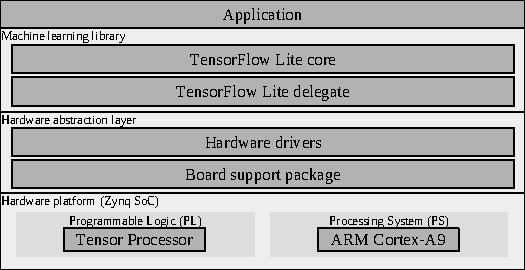
\includegraphics[width=0.5\textwidth]{./chapters/cnn_accelerator/figures/sw_stack.pdf}
	\caption{High level embedded software architecture.}
	\label{fig:sw_stack}
\end{figure}

\begin{figure}[t!]
	\centering
	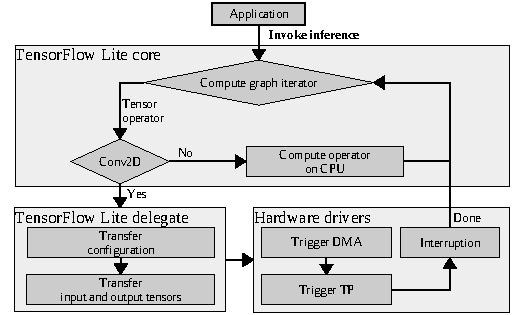
\includegraphics[width=0.5\textwidth]{./chapters/cnn_accelerator/figures/sw_stack_flowchart.pdf}
	\caption{Software flowchart.}
	\label{fig:sw_stack_flowchart}
\end{figure}

\subsection{Embedded software architecture}
The software architecture is a layered object-oriented application framework written in C++, see \fig{fig:sw_stack} and \fig{fig:sw_stack_flowchart}. Description of the software layers is as follows:
\begin{itemize}
	\item \emph{Application}: As the highest level of abstraction, this software layer implements the analytics application, this invokes the \gls{ml} library.
	\item \emph{Machine learning library}: This software layer offers a comprehensive high level \gls{api} for \gls{ml} inference. This layer consist of TensorFlow Lite micro, this is modified to implement the delegate software interfaces for the proposed hardware accelerator.
	\item \emph{Hardware abstraction layer}: This layer consist of the hardware drivers used in the TFLite delegate interfaces. This software layer handles initialization and runtime operation of the \gls{tp} and \gls{dma}.
\end{itemize}
\section{Experimental Results}
\label{sec:experimental_results}
This section presents experimental results using a low-power/low-cost sensor analytics application. A \gls{cnn}-regression model is proposed to predict x- y- coordinates of acoustic emissions based on piezoelectric vibrations. Quantitative and qualitative aspects of the analytics are compared using floating-point 32-bit, fixed-point 8-bit, Hybrid-Logarithmic 6-bit, and Hybrid-Float6.

To demonstrate the proposed concept, the \gls{cnn} model is deployed in the smallest Zynq \gls{soc} \gls{fpga} device for low-power inference. The performance of the \gls{tp} synthesized with standard \gls{fp} (using Xilinx LogiCORE IPs) and Hybrid-Float6 design.

\subsection{Sensor Analytics Application}
The analytics model is designed to predict x- y- coordinates of acoustic emissions on a metal plate. The metal plate is in the presence of noise disturbance to simulate realistic conditions. This subsection presents the structure for experimental setup, data sets, and the \gls{cnn}-regression model.

\subsubsection{Experimental Setup}
The experiment uses eight piezoelectric sensors (Vallen Systeme VS900) attached with magnetic holders on a metal plate ($\unit[90]{cm}\times\unit[86.6]{cm}\times\unit[0.3]{cm}$). The VS900 devices can operate either in active or passive mode. Six VS900 are used in passive mode as acoustic sensors and two in active mode to produce acoustic emissions. These acoustic emissions simulate anomalies on x- y- coordinates as well as the noise disturbance on the system. See \fig{fig:data_set}(a). To create data sets, the samples of acoustic emissions are labeled with their coordinates.

\subsubsection{Data Sets}
The data sets are recorded applying pulses on the metal plate, the x- y- coordinates of these pulses are used as labels. The pulses for training and validation data sets are shown in \fig{fig:data_set}(b) and \fig{fig:data_set}(c), respectively. The pulses for training and validation data sets are mutually exclusive, this exclusion is represented by the cross symbols in \fig{fig:data_set}(c). This creates a grid layout used to collect samples for the data sets. This grid is $10\times10$ divisions, these are on the metal plate area ($\unit[90]{cm}\times\unit[86.6]{cm}$). This grid does not consider the four corners as they are used for magnetic holders.

\begin{figure}[t!]
	\centering
	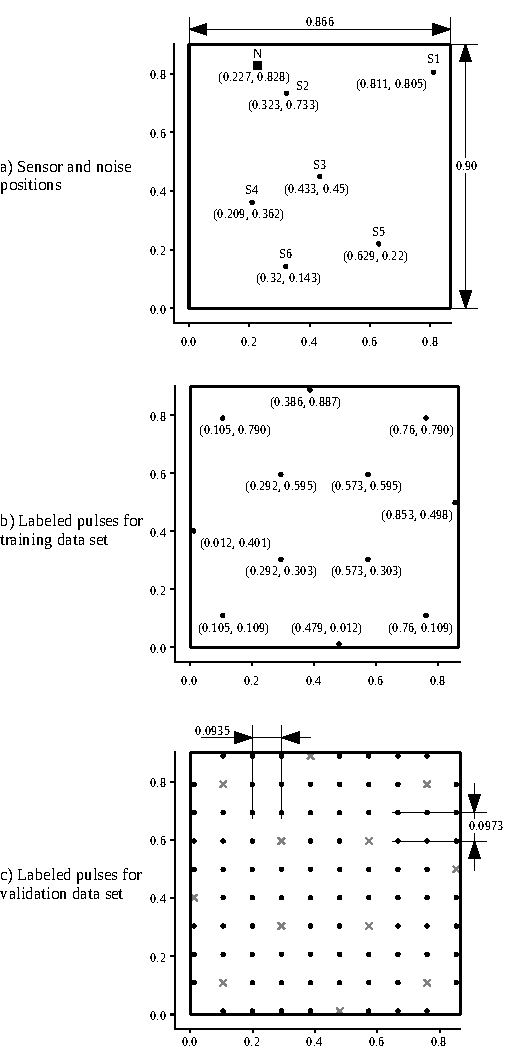
\includegraphics[width=0.5\textwidth]{./chapters/cnn_accelerator/figures/histograms/data_set.pdf}
	\caption{Experimental setup for sensor analytics on structural health monitoring, all lengths are in meters (m).}
	\label{fig:data_set}
\end{figure}

In order to create reproducible acoustic emissions, this demonstration uses 9-cycle sine pulse in a Hanning window with central frequency $f_\mathrm{c}$ (narrow-banded in the frequency domain). This experiment assumes guided Lamb waves based on the plate structure. The narrow-band behavior also reduces the dispersion of the acoustic emission waves~\cite{hannwindowsine}. The waveform can be expressed as a function of time $t$ as follows:

\begin{equation}
x_\mathrm{pulse}(t) = \frac{1}{2} \Big(1-\cos{\frac{f_\mathrm{c} t}{5}} \Big) A_0 \sin{f_\mathrm{c} t}.
\end{equation}

To generate the data sets, slightly different pulse amplitudes and frequencies for excitation are used. The pulse frequency $f_c$ is varied in $\unit[1]{kHz}$ steps between $\unit[300]{kHz}$ and $\unit[349]{kHz}$ and the amplitude $A_0$ is varied in $\unit[0.1]{V}$ steps between $\unit[2.6]{V}$ and $\unit[3.5]{V}$. This produces 500 different pulses for each of the excitation points.

The signals for labeled pulses and noise disturbance are generated by \glspl{awg}. The sensor signals are recorded via a Vallen AMSY-6 measurement system with a resolution of 18 bits and a sampling rate of $f_\mathrm{S} =\unit[10]{MHz}$. The disturbance signal is gaussian noise with amplitudes between 0-3 V. This noise is applied via the piezoelectric device $N$ at $x=\unit[0.227]{m}$ and $y=\unit[0.828]{m}$, see \fig{fig:data_set}(a).

To obtain frequency components, the sampled pulses are converted into the frequency-time domain using the \gls{stft}. This is calculated as follows~\cite{stft_lit}:

\begin{flalign}
\label{stft_eq2}
\mathcal{F}_{m,k}^\gamma= \sum_{n=0}^{N-1} x[n] \cdot \gamma^*[n-m\Delta M]\cdot \mathrm{e}^{\frac{-j 2 \pi k n }{N}}
\end{flalign}

Here $x[n]$ describes a discrete-time signal and $\gamma^*[n-m\Delta M]\cdot \mathrm{e}^{\frac{-j 2 \pi k n }{N}}$ the time- and frequency-shifted window function inside the considered interval $[0 , N-1]$. $\Delta M$ describes the time shift and $N$ the transformation window. Since only discrete frequencies and time points are considered, $m = 0,1,...,M-1$ is valid. For pictorial representation, the magnitude of the complex-valued \gls{stft} is employed in a spectrogram $\mathcal{S}_{m,k}$:

\begin{flalign}
\label{stft_eq3}
\mathcal{S}_{m,k}= \left|\mathcal{F}_{m,k}^\gamma\right|^2 = \left|\sum_{n=0}^{N-1} x[n] \cdot \gamma^*[n-m\Delta M]\cdot \mathrm{e}^{\frac{-j 2 \pi k n }{N}} \right|^2
\end{flalign}

In addition, these spectrograms are scaled in decibels. The spectrogram in decibels $\mathcal{S}_{m,k,\mathrm{dB}}$ produces $\mathcal{S}_{m,k,\mathrm{dB}}= 20 \cdot \mathrm{log}_{10}(\mathcal{S}_{m,k})$. For conversion of data, the experiment uses a signal length of 400 \textmu s (75 \textmu s pretrigger and 325 \textmu s post trigger). Thus, the arrival times of the pulses are included in the spectrogram for all channels and labeled positions. This uses Blackman window function~\cite{blackman_window}, \gls{fft} length of 32 samples, and overlap of 8 samples. The spectrograms are calculated for frequencies in the range of \unit[100]{kHz} to \unit[500]{kHz}. This produces a spectrogram size of 8x16 (8 frequency bins, 16 time values).

In order to generate larger data sets, four further variants are created with time shifts of 15 \textmu s/ 30 \textmu s/ 45 \textmu s/ 60 \textmu s. Subsequently, all spectrograms are converted to grayscale with scaling between \unit[-100]{dB} and \unit[-40]{dB}, see \fig{fig:spectrograms}.

In overall, the data set has a size of 1,440,000 images. This is the result of 500 (pulses) $\cdot$ 5 (spectrograms) $\cdot$ 6 (listening sensors) $\cdot$ 96 (excitation points).

\begin{figure}[t!]
	\centering
	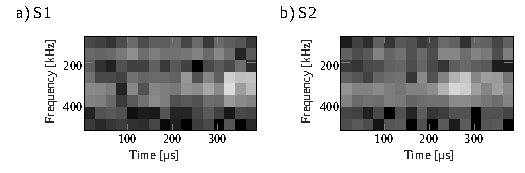
\includegraphics[width=0.5\textwidth]{./chapters/cnn_accelerator/figures/histograms/spectrograms.pdf}
	\caption{Spectrograms of sensors $S_1, S_2$ converted to grayscale for pulses at $x =0.105$ m, $y = 0.109$ m with noise disturbance.}
	\label{fig:spectrograms}
\end{figure}

\subsubsection{CNN-Regression Model}
The data analytics is implemented with a \gls{cnn}-regression model, see \fig{fig:model}. The structure of the model is described below:

\begin{enumerate}[label=\alph*)]
\item Input tensor. This is composed of spectrograms from the sensor signals. The tensor shape is defined by $S \times T \times F$, where $S$ is the number of sensors, and $T \times F$ is the time-frequency resolution of the spectrograms, see \fig{fig:model}(a).

\item Feature extraction. This is composed of three blocks of convolution, batch normalization, and max-pooling layers, see \fig{fig:model}(b). The number of channels in the convolution layers are defined by the hyper-parameters $A$, $B$, and $C$.

\item Regression function. This is an arbitrary function implemented with two fully connected layers and an output layer with linear activation, see \fig{fig:model}(c).
\end{enumerate}


\begin{figure}[t!]
	\centering
	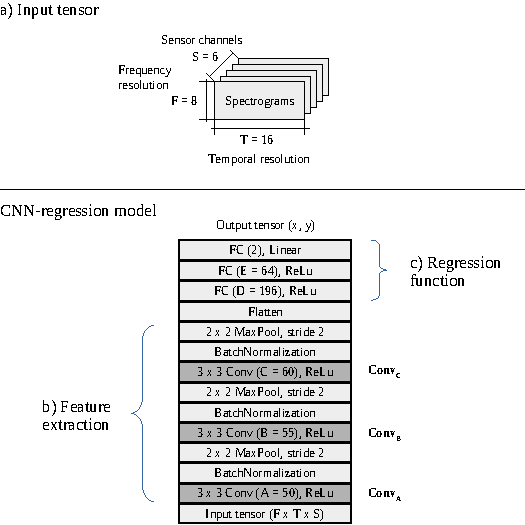
\includegraphics[width=0.5\textwidth]{./chapters/cnn_accelerator/figures/models.pdf}
	\caption{CNN-regression model for sensor analytics.}
	\label{fig:model}
\end{figure}


\subsection{Training}
\subsubsection{Base Model}
The model in \fig{fig:model} is trained using Adam algorithm with iterative search. The Adam optimizer is configured with the default settings presented in \cite{kingma2014adam}: $\alpha = 0.001$, $\beta_1 = 0.9$, $\beta_2 = 0.999$, and $\epsilon = 1\mathrm{e}{-8}$. The training-cycle has a patience of 10 iterations before stop, the optimizer is executed with early stop patience of 10 epochs, and mini-batch size of 512 samples. This is applied using the method described in \Algo{alg:training} with $N_I = 10$, $N_E=10$, $B_{size}=512$.

The training results are illustrated in \fig{fig:optimization}(a). In this optimization, the initial and the final models achieve $MSE=\unit[0.0135]{m^2}$ and $MSE=\unit[0.0122]{m^2}$, respectively. The $MSE$ is calculated with the Euclidean distance (loss) between the real/expected and the predicted/inferred coordinates. The initial model is obtained at the first early stop (after 10 epochs). In each stop, the moving averages of the Adam optimizer get re-initialized. This facilitates searching for better local minima. The model gets saved/updated when finding a better minimum.

\begin{figure}[h!]
	\centering
	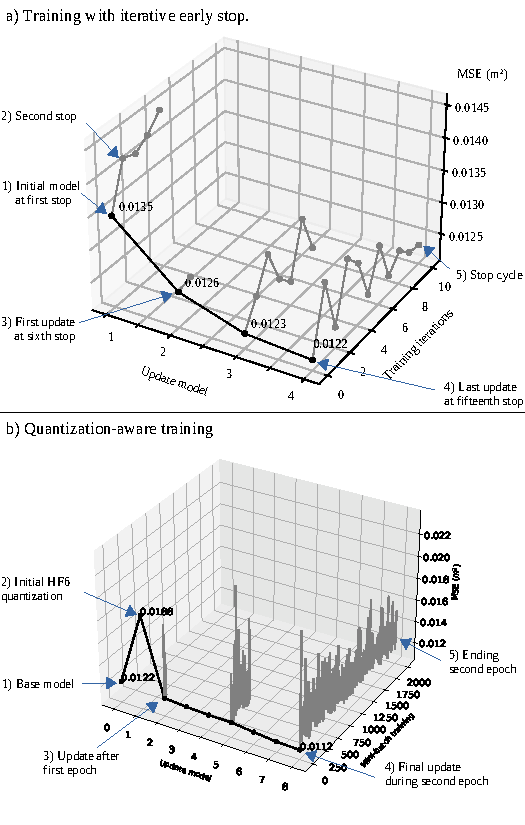
\includegraphics[width=0.5\textwidth]{./chapters/cnn_accelerator/figures/histograms/training_and_quantization.pdf}
	\caption{Training results.}
	\label{fig:optimization}
\end{figure}

The final model achieves $MSE=\unit[0.0122]{m^2}$, which corresponds to $MAE=\unit[0.0955]{m}$. See \fig{fig:model_evaluation}(a). In total, the training takes 379 epochs in 25 cycle-search iterations. The first search takes 43 epochs for the initial model and subsequent search iterations take an average of 14 epochs. The total time is 53 minutes using a \gls{pc} with AMD Ryzen 5 5600H and NVIDIA GeForce RTX 3050 \gls{gpu}.

\begin{figure}[h!]
	\centering
	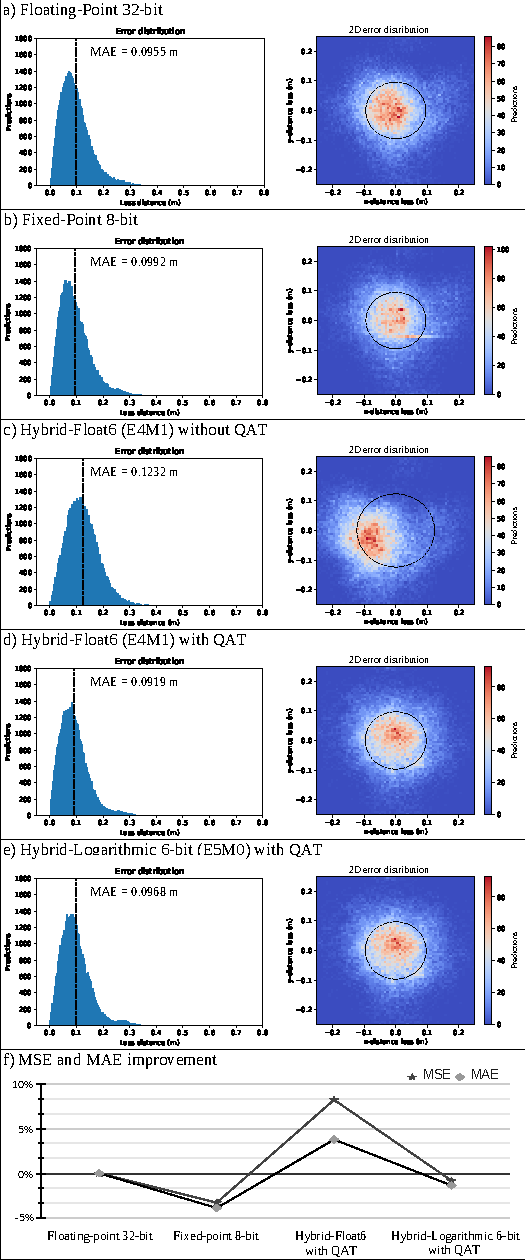
\includegraphics[width=0.5\textwidth]{./chapters/cnn_accelerator/figures/histograms/model_evaluation.pdf}
	\caption{Performance of the model with different data representations.}
	\label{fig:model_evaluation}
\end{figure}

\subsubsection{TensorFlow Lite 8-bit Quantization}
This optimization method converts filter and bias tensors as well as activation maps to 8-bit integer representation, this allows inference using integer-only arithmetic~\cite{hannwindowsine}. In this research, this quantization is applied only to the convolution layers as they are the compute bound operations. Other layers employ 32-bit \gls{fp} representation.

In the compute graph, the input and output feature maps are glued with linear quantization at the input and output of the \emph{Conv2D} operations.

The base model is quantized using the TensorFlow Lite library with integer-only quantization on the \emph{Conv2D} tensor operations. The filter and bias tensors are represented by 8-bit and 32-bit signed integers, respectively. The input and output activation maps are represented by 8-bit signed integer. The TensorFlow quantization includes two additional vectors (output-multiplier and output-shift coefficients), these two vectors are the same shape as the bias vector with 32-bit integer representation.

This model achieves $MSE=\unit[0.0126]{m^2}$ and $MAE=\unit[0.0992]{m}$. See \fig{fig:model_evaluation}(b). The MAE increases 5.1\% of the base model. We attribute this degradation to the 8-bit quantization on the \emph{Conv2D} layers.

\subsubsection{Inference of non-quantized models on HF6 hardware}
To demonstrate backward compatibility, the inference quality of the base model is measured without quantization on the \gls{hf6} hardware. See \fig{fig:model_evaluation}(c). This obtains $MSE=\unit[0.0188]{m^2}$ and $MAE=\unit[0.1232]{m}$. The MAE increases 29.5\% of the base model. We attribute this degradation to the rounding errors of non-quantized filters and bias in \emph{Conv2D} layers.

\subsubsection{Quantization-Aware Training for HF6 hardware}
The \gls{qat} is a post-training optimization. This has been run during two epochs with mini-batch size of 10 samples. This quantization is executed targeting the HF6 format: 4-bit exponent and 1-bit mantissa. This is applied to filter and bias tensors of \emph{Conv2D} layers. This method is described in \Algo{alg:quantization_integration} with $N_{ep}=2$, $B_{size}=10$, $E_{size}=4$, $M_{size}=1$. The optimization results are illustrated in \fig{fig:optimization}(b).

The resulting model achieves $MSE=\unit[0.0112]{m^2}$ and $MAE=\unit[0.0919]{m}$. This corresponds to an error reduction of 8.2\% and 3.77\%, respectively. We attribute this improvement to the regularization effect. See \fig{fig:model_evaluation}(d). The \gls{qat} time is 185 minutes.


\subsubsection{Quantization-Aware Training for Hybrid-Logarithmic 6-bit}
For the sake of quality comparison with logarithmic quantization, the model with 6-bit logarithmic representation is generated. See \fig{fig:floating}(e). This quantization matches the bit size of \gls{hf6}. The filter and bias tensors of \emph{Conv2D} layers are quantized with the 6-bit logarithmic format: 1-bit sign, 5-bit signed exponent, and 0-bit mantissa. This is applied using the method described in \Algo{alg:quantization_integration} with $N_{ep}=2$, $B_{size}=10$, $E_{size}=5$, $M_{size}=0$.

The model achieves $MSE=\unit[0.0123]{m^2}$ and $MAE=\unit[0.0968]{m}$, which correspond to an error increase of 0.82\% and 1.36\%, respectively. We attribute this degradation to the 6-bit logarithmic quantization lacking fractional bits. See \fig{fig:model_evaluation}(e).

A summary of improvement-degradation of MSE and MAE with different data representations is presented in \fig{fig:model_evaluation}(f).

\subsection{Hardware Design Exploration}
The proposed hardware/software co-design is demonstrated on the Zynq-7007S \gls{soc} on the MiniZed development board. This \gls{soc} integrates a single ARM Cortex-A9 \gls{ps} and a \gls{pl} equivalent to Xilinx Artix-7 \gls{fpga} in a single chip~\cite{xilinx2015zynq}. The Zynq-7007S \gls{soc} architecture maps the custom logic and software in the \gls{pl} and \gls{ps}, respectively.

In this platform, the proposed hardware/software architecture is implemented to deploy the sensor analytics application. The desired model is converted to TensorFlow Lite (floating-point) and deployed on the embedded software as a hex dump as a C array. The Zynq-7007S \gls{soc} executes inference with TensorFlow Lite on the \gls{ps}. The computational workload of convolution layers is delegated to the dedicated hardware.

\subsubsection{Benchmark on Embedded CPU}
First, the performance of the embedded \gls{cpu} is explored for inference without hardware acceleration. In this case, TensorFlow Lite creates the \gls{cnn} model as a sequential compute graph executing all computation on the \gls{cpu} (ARM Cortex-A9) at $\unit[666]{MHz}$ with power dissipation of $\unit[1,187]{W}$.

The compute performance and run-time inference of the \gls{cpu} are shown in \Tab{tab:performance}(a) and \fig{fig:runtime}(a), respectively.

\subsubsection{Benchmark on Tensor Processor Synthesized with Xilinx LogiCORE IP for Floating-Point Computation}
For this design, the TP is implemented with standard Xilinx \gls{fp} hardware prior synthesis. The design parameters for the maximum required accelerator on-chip size are:
\begin{itemize}
	\item Max convolution kernel size: $K_W = K_H = 3$.
	\item Max input tensor width: $W_I = 16$.
	\item Max input and output channels: $C_I = 55$, $C_O = 60$.
	\item Filter and bias bit size: $BitSize_F=BitSize_B=32$.
	\item Input tensor bit size: $BitSize_I=32$.
\end{itemize}

Using equations from Section \ref{sec:memory_utilization}, the on-chip memory utilization are $Input_M=84,480$b, $Filter_M=950,400$b, and $Bias_M=1,920$b. Hence, the required on-chip memory buffer size is $TP_B=1,036,800$b.

The post-implementation resource utilization and power dissipation are presented in \Tab{tab:resource_utilization}(a). The complete hardware platform utilizes 83\% of BRAM, this includes the on-chip memory requirements of the \gls{tp}, \gls{dma}, and AXI interconnects. The total available on-chip memory (BRAM) on the Zynq-7007S \gls{soc} is $\unit[1.8]{Mb}$. After hardware syntheses, the estimated power dissipation of the \gls{tp} is $\unit[85]{mW}$ at $\unit[200]{MHz}$ (this estimation is provided by Xilinx Vivado).

\begin{table}[!h]\centering
	\caption{Resource utilization and power dissipation on the Zynq-7007S SoC.}\label{tab:resource_utilization}
	\scriptsize
	\begin{tabular}{lrrrrrr}\toprule
		\multirow{2}{*}{\textbf{TP engine}} &\multicolumn{4}{c}{\textbf{Post-implementation resource utilization}} &\multirow{2}{*}{\textbf{Power (W)}} \\\cmidrule{2-5}
		&\textbf{LUT} &\textbf{FF} &\textbf{DSP} &\textbf{BRAM 36Kb} & \\\midrule
		\multirow{2}{*}{(a) Floating-Point} &5,578 &8,942 &23 &41.5 &\multirow{2}{*}{1.429} \\
		&39\% &31\% &35\% &\textbf{83\%} & \\
		\multirow{2}{*}{(b) Hybrid-Float6} &7,313 &10,330 &20 &15 &\multirow{2}{*}{1.424} \\
		&51\% &36\% &30\% &\textbf{30\%} & \\
		\bottomrule
	\end{tabular}
\end{table}

The compute performance and inference schedule of the model on this hardware implementation are shown in \Tab{tab:performance}(b) and \fig{fig:runtime}(b), respectively. During run-time, the software (TensorFlow Lite) delegates computation to the \gls{tp} as dedicated hardware for \emph{Conv2D} tensor operations.

The implementation of the dot-product with standard \gls{fp} engine (IEEE 754 arithmetic) utilizes proprietary multiplier and adder floating-point operator cores. Vivado \gls{hls} implements \gls{fp} arithmetic operations by mapping them onto Xilinx LogiCORE IP cores, these \gls{fp} operator cores are instantiated in the resultant \gls{rtl}~\cite{hrica2012floating}. In this case, the implementation of the dot-product with the standard \gls{fp} computation reuses the multiplier and adder cores in different compute sections of the \gls{tp}. The post-implementation resource utilization and power dissipation of the individual floating-point operator cores are shown in \Tab{tab:LogiCORE}.

\begin{table}[!t]\centering
	\caption{Compute performance of the CPU and TP on each Conv2D tensor operation. This table presents: tensor operation, computational cost in mega floating-point operations (MFLOP), latency, throughput, power efficiency, and estimated energy consumption as the energy delay product (EDP).}\label{tab:performance}
	\scriptsize
	\begin{tabular}{lrrrrrr}\toprule
		\textbf{Operation} &\textbf{MFLOP} &\textbf{t (ms)} &\textbf{MFLOP/s} &\textbf{MFLOP/s/W} &\textbf{EDP (mJ)} \\\midrule
		& &\multicolumn{4}{l}{\textbf{a) CPU (ARM Cortex-A9) @666MHz, 1.187 W}} \\
		Conv\textsubscript{A} &0.691 &112.24 &6.16 &5.19 &133.23 \\
		Conv\textsubscript{B} &1.584 &213.13 &7.43 &6.26 &252.99 \\
		Conv\textsubscript{C} &0.475 &46.59 &10.20 &8.59 &55.31 \\
		& &\multicolumn{4}{l}{\textbf{b) TP (Floating-Point engine) @200MHz, 85 mW}} \\
		Conv\textsubscript{A} &0.691 &12.49 &55.34 &651.11 &1.06 \\
		Conv\textsubscript{B} &1.584 &16.39 &96.66 &1,137.20 &1.39 \\
		Conv\textsubscript{C} &0.475 &3.59 &132.44 &1,558.13 &0.30 \\
		& &\multicolumn{4}{l}{\textbf{c) TP (Hybrid-Float6 engine) @200MHz, 84 mW}} \\
		Conv\textsubscript{A} &0.691 &6.92 &99.81 &1,188.24 &0.58 \\
		Conv\textsubscript{B} &1.584 &4.41 &358.94 &4,273.09 &0.37 \\
		Conv\textsubscript{C} &0.475 &0.99 &482.44 &5,743.29 &0.08 \\
		\bottomrule
	\end{tabular}
\end{table}

\begin{figure}[t!]
	\centering
	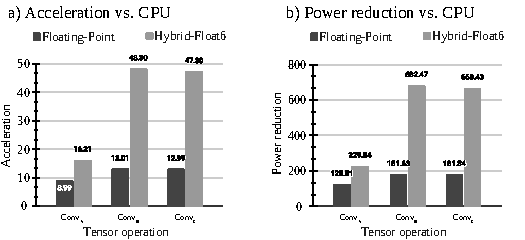
\includegraphics[width=0.5\textwidth]{./chapters/cnn_accelerator/figures/power_breakdown/acceleration_power_reduction.pdf}
	\caption{Inference acceleration and power reduction on the TP with floating-point and HF6 vs. CPU on the Zynq-7007S SoC.}
	\label{fig:acceleration}
\end{figure}


\begin{table}[!h]\centering
	\caption{Resource utilization and power dissipation of individual multiplier and adder floating-point (IEEE 754) operator cores (Xilinx LogiCORE IP).}\label{tab:LogiCORE}
	\scriptsize
	\begin{tabular}{lrrrrrr}\toprule
		\textbf{Core operation} &\textbf{DSP} &\textbf{FF} &\textbf{LUT} &\textbf{Latency (clk)} &\textbf{Power (mW)} \\\midrule
		Multiplier &3 &151 &325 &4 &7 \\
		Adder &2 &324 &424 &8 &6 \\
		\bottomrule
	\end{tabular}
\end{table}



\subsubsection{Tensor Processor Synthesized with Hybrid-Float6 Hardware Architecture}
To demonstrate the proposed design, the \gls{tp} with \gls{hf6} hardware reuses the standard \gls{fp} design parameters with the following variation for the 6-bit representation in filter and bias: $BitSize_F=BitSize_B=6$.

Using equations from Section \ref{sec:memory_utilization}, the on-chip memory requirements for the hardware accelerator are $Input_M=\unit[84,480]{b}$, $Filter_M=\unit[178,200]{b}$, $Bias_M=\unit[360]{b}$. Hence, the required on-chip memory buffer size is $TP_B=\unit[263,040]{b}$.

The post-implementation resource utilization and power dissipation are presented in \Tab{tab:resource_utilization}(b). The complete hardware platform utilizes 30\% of BRAM, this includes the on-chip memory requirements of the \gls{tp}, \gls{dma}, and AXI interconnects. The estimated power dissipation of the \gls{tp} is $\unit[84]{mW}$ at $\unit[200]{MHz}$ (this estimation is provided by Xilinx Vivado).

The compute performance and inference schedule of the model on this hardware implementation are shown in \Tab{tab:performance}(c) and \fig{fig:runtime}(c), respectively. \Fig{fig:acceleration} presents a comparison of the acceleration and the reduction of power dissipation between standard \gls{fp} and \gls{hf6} hardware implementations.

This deployment does not require model treatment for hardware compatibility. For backward compatibility, the 6-bit \gls{fp} representation is wrapped into the standard \gls{fp}. The dedicated hardware design extracts the 6-bit format automatically to perform computation.

\begin{figure}[t!]
	\centering
	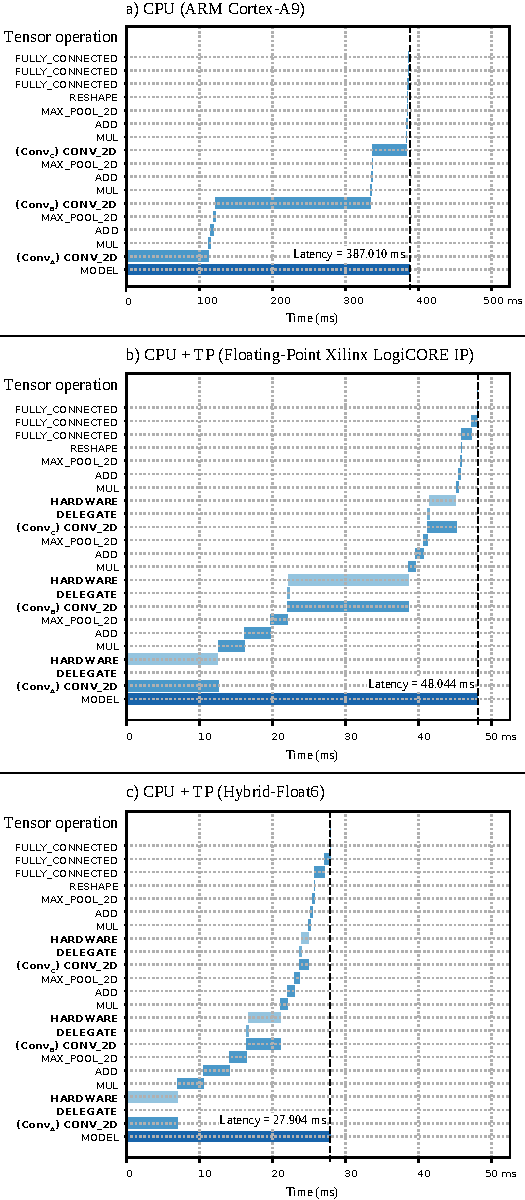
\includegraphics[width=0.5\textwidth]{./chapters/cnn_accelerator/figures/runtime/runtime.pdf}
	\caption{Run-time inference of TensorFlow Lite on the Zynq-7007S SoC. (a) CPU ARM Cortex-A9 at $\unit[666]{MHz}$, (b) cooperative CPU + TP with floating-point Xilinx LogiCORE IP at $\unit[200]{MHz}$, and (c) cooperative CPU + TP with Hybrid-Float6 at $\unit[200]{MHz}$.}
	\label{fig:runtime}
\end{figure}

\subsection{Discussion}
\subsubsection{Training and Quantization}
The training with iterative early stop obtains a model with enhanced accuracy than standard early stop. This method iteratively resets the moving averages of Adam's optimizer, which helps to iteratively search for better local minima. This iterative search is suitable for models with low computational cost.

The TensorFlow Lite 8-bit quantization preserves the overall model accuracy. In some cases, the associated regularization effect can improve the accuracy. However, the error distribution in \gls{cnn} linear regressions gets slightly degraded. In particular, 8-bit quantized output layers incur in discrete-degradation patterns, \fig{fig:2d_error_distribtion}(b) shows this effect on three different models. Vertical and horizontal patterns appear in the error distribution of 8-bit fixed-point quantization. We attribute this effect to the 8-bit resolution in the activation maps. In the case of \gls{hf6} quantization, the activation maps are represented by floating-point preventing this degradation.

The proposed 6-bit \gls{fp} representation (E4M1) improves latency, hardware area, and power dissipation, while preserving model accuracy. For comparison, in our application, this number format produces better results than the 6-bit logarithmic representation (E5M0). This is demonstrated in \Fig{fig:model_evaluation}(d) and \Fig{fig:model_evaluation}(e).

In \cite{lai2017deep}, Lai \textit{et al.} demonstrated that 4-bit exponent and X-bit mantissa preserves accuracy on SqueezeNet, AlexNet, GoogLeNet, and VGG-16. To contribute on this, I investigated 4-bit exponent and 1-bit mantissa to ALL-CNN-C~\cite{springenberg2014striving}, this produces an accuracy degradation of 1.39\% and 0.11\% with \gls{qat}. While applying 6-bit logarithmic produces a degradation of 11.18\% and 7.22\% with \gls{qat}.

\begin{figure}[t!]
	\centering
	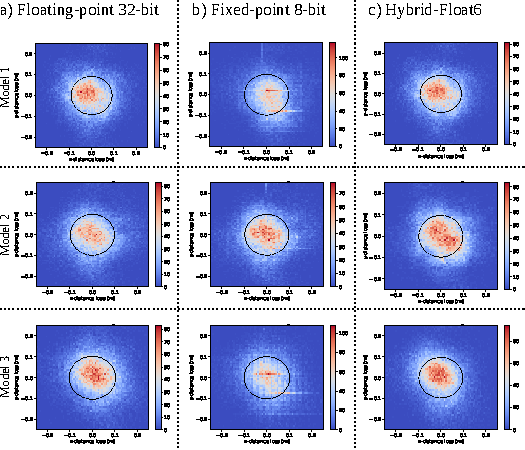
\includegraphics[width=0.5\textwidth]{./chapters/cnn_accelerator/figures/histograms/2D_error_distribtion.pdf}
	\caption{2D error distribution of three CNN-regression models.}
	\label{fig:2d_error_distribtion}
\end{figure}

\subsubsection{Implementation and Performance}
The proposed \gls{hf6} implementation reduces on-chip memory and \gls{dsp} utilization while slightly increasing \glspl{ff} and \glspl{lut} compared to the standard \gls{fp} implementation. See \Tab{tab:resource_utilization} and \Fig{fig:resource_utilization}. This is attributed to the \gls{hf6} logic implementation using \gls{ff} and \gls{lut}, while the \gls{fp} logic implementation uses Xilinx LogiCORE IPs mainly with \glspl{dsp}.

The compute performance of the \gls{cpu} and \gls{tp} on each convolution layer is presented in \Tab{tab:performance} and \fig{fig:acceleration}. 
The peak acceleration and power efficiency of the \gls{tp} with standard \gls{fp} (Xilinx LogiCORE IP) is $13\times$ and \unit[1,558.13]{MFLOPS/s/W}, respectively. While the peak acceleration and power efficiency of the \gls{tp} with \gls{hf6} is $48.3\times$ and \unit[5,743.29]{MFLOPS/s/W}, respectively. The \gls{hf6} hardware demonstrates an improvement of $3.7\times$ in acceleration and power efficiency with respect to the standard \gls{fp} hardware. See \Fig{fig:acceleration}.

The estimated power dissipation on the \gls{soc} is presented in \fig{fig:power}. This shows a very similar breakdown of power dissipation in both implementations. However, the energy efficiency is increased due to the reduced latency in \gls{hf6} hardware. A comparison of related work is presented in \Tab{tab:comparison}.

\begin{figure}[h!]
	\centering
	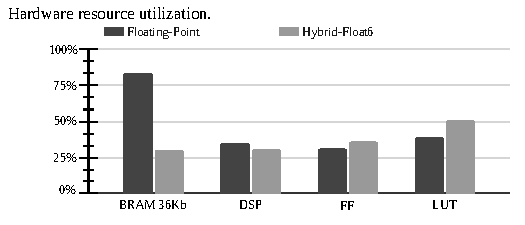
\includegraphics[width=0.5\textwidth]{./chapters/cnn_accelerator/figures/power_breakdown/resource_utilization.pdf}
	\caption{Hardware resource utilization on the Zynq-7007S SoC.}
	\label{fig:resource_utilization}
\end{figure}

\begin{figure}[h!]
	\centering
	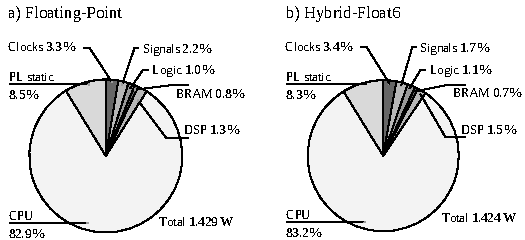
\includegraphics[width=0.5\textwidth]{./chapters/cnn_accelerator/figures/power_breakdown/power_breakdown.pdf}
	\caption{Estimated power dissipation on the Zynq-7007S SoC with PS at $\unit[666]{MHz}$ and PL at $\unit[200]{MHz}$.}
	\label{fig:power}
\end{figure}

The run-time inference of TensorFlow Lite on the \gls{soc} is illustrated in \Fig{fig:runtime}. This shows the convolution layers as the compute-bound operations. The proposed embedded platform is a cooperative system where the convolution operations are delegated to the dedicated hardware accelerator. The ARM \gls{cpu} obtains a latency of \unit[387]{ms} (\unit[2.58]{FPS}). The platform with standard \gls{fp} hardware obtains a latency of \unit[48]{ms} (\unit[20.8]{FPS}), while the implementation with \gls{hf6} obtains a latency of \unit[27.9]{ms} (\unit[35.84]{FPS}). These represent an overall acceleration of $8\times$ and $13.87\times$ over the \gls{cpu}, respectively.

This design facilitates \gls{ml} compatibility/portability as the 6-bit \gls{fp} is wrapped in the standard \gls{fp} representation. The dedicated hardware design extracts the 6-bit format automatically and performs computation.

\subsubsection{SoC Design and Compatibility}
The proposed design is an alternative for high accuracy and low-power floating-point inference. The system runs as a cooperative hardware/software mechanism. This architecture delegates compute-bound tensor operations to a hardware accelerator.

The hybrid 32-bit \gls{fp} and 6-bit \gls{fp} quantization enables high quality of results and backward \gls{ml} compatibility. Backwards \gls{ml} compatibility gives portability from training to inference. This enables to run inference of \gls{hf6} quantized models on standard \gls{fp} hardware and vise versa. The proposed \gls{hf6} architecture allows to compute inference of non-quantized floating-point \gls{ml} models for rapid deployment; however, this will incur in accuracy degradation depending on the resilience of the model, see \Fig{fig:model_evaluation}(c).

\begin{table*}[!t]\centering
	\caption{Comparison of hardware implementation with related work.}\label{tab:comparison}
	\scriptsize
	\begin{tabular}{lrrrrrr}\toprule
		Platform &Chunsheng \textit{et al.} \cite{mei2017200mhz} &Chen \textit{et al.} \cite{wu2021low} &BFP \cite{lian2019high} &Paolo \textit{et al.} \cite{meloni2019cnn} &This work \\\midrule
		Device &XC7VX690T &XC7K325T &XC7VX690T &XC7Z007S &XC7Z007S \\
		Year &2017 &2019 &2019 &2019 &2023 \\
		Dev. kit cost &\$7,494 &\$1,299 &\$7,494 &\$89 &\$89 \\
		Format (activation/weight) &FP 16-bit &FP 8-bit / 8-bit &FP 16-bit / 8-bit &INT 16-bit &FP 32-bit / 6-bit \\
		Frequency (MHz) &200 &200 &200 &80 &200 \\
		Peak power efficiency (GFLOP/s/W) &18.72 &115.40 &82.88 &2.98 &5.74 \\
		Peak throughput (GFLOP/s) & 202.42 & 1086.8 & 760.83 &  10.62& 0.482\\
		Wall plug power (W) &10.81 &9.42 &9.18 &2.5 &2.3 \\
		BRAM 36Kb utilization &196.5 &234.5 &913 &44 &15 \\
		DSP utilization &1728 &768 &1027 &54 &20 \\
		\bottomrule
	\end{tabular}
\end{table*}
\section{Conclusions}
\label{sec:conclusions}
This chapter presents the Hybrid-Float6 quantization and its dedicated hardware accelerator for floating-point \gls{cnn} computation. Feature maps and weights are represented by 32-bit and 6-bit \gls{fp}, respectively. The 6-bit \gls{fp} format is composed of 1-bit sign, 4-bit exponent, and 1-bit mantissa. The 1-bit mantissa enables low-power \gls{mac} implementations by reducing the mantissa multiplication to a multiplexer-adder operation. The intrinsic error tolerance of neural networks is exploited to further reduce the hardware design with approximation. This approach improves latency, hardware area, and energy consumption. To preserve accuracy, a \gls{qat} training method is presented that, based on regularization effects can improve accuracy. A lightweight \gls{tp} implementing a pipelined vector dot-product is presented. For \gls{ml} compatibility/portability, the 6-bit \gls{fp} is wrapped in the standard floating-point format, which is automatically extracted by the proposed hardware. The hardware/software architecture is compatible with TensorFlow Lite. To evaluate the applicability of this approach, it is presented a \gls{cnn}-regression model for anomaly localization in a \gls{shm} application based on acoustic emissions. The embedded hardware/software framework is demonstrated on XC7Z007S as the smallest Zynq-7000 \gls{soc}, suitable for low-power \gls{iot} applications. The proposed architecture achieves a peak power efficiency and acceleration on convolution layers of \unit[5.7]{GFLOPS/s/W} and $48.3\times$, respectively.




\chapter{Conclusion and Outlook}
\label{chap.conclusion}
\minitoc
The field of artificial intelligence is launching an era characterized by the prevalence of ubiquitous connected devices. To ensure the sustainability of this transformation, it is crucial to harmonize computational accuracy with energy efficiency and the compatibility of hardware solutions. This dissertation focuses on enhancing the efficiency of AI hardware engines, taking into account these considerations.

\section{State-of-the-art challenges and solutions}
Widely used \gls{ai}/\gls{ml} algorithms, \glspl{snn} and \glspl{cnn}, come with elevated computational and energy demands. The intrinsic error resilience of these algorithms brings "approximate computing" paradigms, such as quantization, to the forefront, offering efficiency enhancements. This research presents cutting-edge methodologies centered on low-power neural network accelerator designs employing custom \gls{fp} computation.

\section{Key Contributions}
\begin{itemize}
	\item \textbf{Hybrid 8-bit Floating-Point and 4-bit Logarithmic Computation}: A hardware design methodology is presented for low-power \gls{sbs} neural networks targeting embedded applications. This approach leverages the intrinsic error resilience of \gls{sbs}, emphasizing a balance between performance and hardware complexity. Significant reductions in run-time, memory footprint, and power consumption are realized, with minimal accuracy trade-offs.
	
	\item \textbf{Hybrid 6-bit Floating-Point Computation}: A novel low-power hardware design technique tailored for resource-constrained applications is presented. The \gls{hf6} quantization strategy, its specialized hardware \gls{mac} unit and tensor processor is showcased. Compatibility with TensorFlow Lite demonstrates its industry relevance and potential for broader adoption.
\end{itemize}

\section{Future Directions}

Future directions focus on optimizing energy efficiency and computational performance for on-device learning techniques. Key strategies include reduced gradient formats for optimized data processing, and exploring reduced hardware architectures with lower-bit formats like Bfloat16 in feature maps. This can significantly optimize memory usage and reduce energy consumption while maintaining \gls{qor}.

Additionally, in this work, there is potential to boost computational throughput by shifting from pipeline to parallel computation structures, augmented by wider memory channels. This approach not only enhances processing speed but also broadens the application scope beyond sensor analytics to a comprehensive range of \gls{ai}/\gls{ml} models for both inference and learning. The goal is to leverage hybrid reduced \gls{fp} quantization, aligning with the need for more energy-efficient on-device learning in various \gls{ai}/\gls{ml} applications.


\section{Final Remarks}
This dissertation delves into design techniques that exploit the intrinsic error resilience of \gls{ai}/\gls{ml} algorithms, focusing on optimal \gls{fp} inference acceleration in resource-constrained embedded systems. Key takeaways include:

\begin{enumerate}
	\item Quantization techniques, particularly those involving reduced floating-point formats, are set to significantly improve hardware designs. These enhancements include acceleration of computation, increased energy efficiency, and optimized chip area. Additionally, they positively impact versatility, portability, and compatibility aspects of hardware solutions.
	
	\item The \gls{mac} module designs presented in this work showcase a balance between computational accuracy and resource efficiency, suitable for resource-constrained embedded devices. This approach has relevance and applicability in both academic research and industrial contexts.
	
	\item The \gls{hf6} quantization approach has the potential to be applicable across the entire spectrum of \gls{ai}/\gls{ml} models. This method enhances energy efficiency, processing speed, and memory footprint, particularly important in the real-world application of \gls{ai}/\gls{ml} technologies.
	
	\item The methodologies showcased for low-power inference acceleration hold significant potential for adaptation on the high computational demands of data centers. Training \gls{ai}/\gls{ml} models using reduced-precision floating-point hardware architectures achieves effects akin to those of \gls{qat} methods. Implementing the proposed techniques in data centers could lead to substantial improvements in energy and resource efficiency.
\end{enumerate}


\appendix
\chapter{Appendix}\label{chap.append}
\section{SbS algorithm}
\label{chap:appendix}

The SbS network inference is described in \Algo{alg:inference}, while spike production and layer update are described in \Algo{alg:spike} and \Algo{alg:update}, respectably.

\begin{algorithm}[t]
	\caption{SbS network inference.} \label{alg:inference}
	
	\begin{algorithmic}
		\SetAlgoLined
		\renewcommand{\algorithmicrequire}{\textbf{input:}}
		\renewcommand{\algorithmicensure}{\textbf{output:}}
		\REQUIRE Layers of the network as $H^l$, where\\
		$l$ is the layer index.
		\REQUIRE $N_{L}$ as the number of layers.
		\REQUIRE $N^l_{X}, N^l_{Y}$ as the size of layers.
		\REQUIRE $N_{Spk}$ as the number of spikes for inference (iterations).
		\ENSURE $H^l$.
		\FOR {$t = 0$ \textbf{to} $N_{Spk}-1$}
		\STATE \textit{Initialization of $H^l(i_X,i_Y,:)$} :
		
		\IF {$t == 0$}
		\FOR {$l = 0$ \textbf{to} $N_{L}-1$}
		\FOR {$i_X = 0, i_Y = 0$ \textbf{to} $N^l_{X}-1, N^l_{Y}-1$}
		\FOR {$i_{H} = 0$ \textbf{to} $N^l_H-1$}
		\STATE $H^l(i_X,i_Y,i_{H}) = 1/N^l_H$
		\ENDFOR
		\ENDFOR
		\ENDFOR
		\ENDIF
		
		\textit{Production of spikes} :
		
		\FOR {$l = 0$ \textbf{to} $N_{L}-1$}
		\IF {$l == 0$}
		\STATE Draw spikes from input \tcp{(\Algo{alg:spike})}
		\ELSE
		\STATE Draw spikes from $H^l$ \tcp{(\Algo{alg:spike})}
		\ENDIF
		
		\ENDFOR
		
		\textit{Update layers} :
		\FOR {$l = 0$ \textbf{to} $N_L - 1$}
		\STATE Update $H^l$ \tcp{(\Algo{alg:update})}
		\ENDFOR
		
		\ENDFOR
	\end{algorithmic} 
\end{algorithm}


\begin{algorithm}[t]
	\caption{Spike production.} \label{alg:spike}
	
	\begin{algorithmic}[1]
		\SetAlgoLined
		\renewcommand{\algorithmicrequire}{\textbf{input:}}
		\renewcommand{\algorithmicensure}{\textbf{output:}}
		\REQUIRE Layer as $H_t\in\mathbb{R}^{N_X \times N_Y \times N_H}$, where\\
		$N_X$ is the layer width,\\
		$N_Y$ is the layer height\\
		$N_H$ is the length of $\vec{h}$ (IP vector).
		\ENSURE Output spikes as $S_t^{out} \in\mathbb{N}^{N_X \times N_Y}$
		
		\FOR {$i_X = 0$, $i_Y = 0$ \textbf{to} $N_X-1$, $N_Y-1$}
		
		
		\STATE \textit{Generate spike} :
		
		\STATE $th = MT19937PseudoRandom()/(2^{32}-1)$
		\STATE $acu = 0$
		\FOR {$i_{H} = 0$ \textbf{to} $N_H-1$}
		\STATE $acu = acu + H_t(i_X,i_Y,i_{H})$
		\IF {$th \leq acu$ \textbf{or} $i_{H} == N_{H}-1$}
		\STATE $S_t^{out}(i_X,i_Y) = i_{H}$
		\ENDIF
		\ENDFOR
		\ENDFOR
	\end{algorithmic} 
\end{algorithm}





\begin{algorithm}[t]
	\caption{SbS layer update.} \label{alg:update}
	
	\begin{algorithmic}[1]
		\SetAlgoLined
		\renewcommand{\algorithmicrequire}{\textbf{input:}}
		\renewcommand{\algorithmicensure}{\textbf{output:}}
		\REQUIRE Layer as $H\in\mathbb{R}^{N_X \times N_Y \times N_H}$, where\\
		$N_X$ is the layer width,\\
		$N_Y$ is the layer height\\
		$N_H$ is the length of $\vec{h}$ (IP vector).
		\REQUIRE Synaptic matrix as $W\in\mathbb{R}^{K_X \times K_Y \times M_H\times N_H}$, where\\
		$K_X \times K_Y$ is the size of the convolution/pooling kernel, \\
		$M_H$ is the length of $\vec{h}$ from previous layer,\\
		$N_H$ is the length of $\vec{h}$ from this layer.  
		\REQUIRE Input spike matrix from previous layer as $S_t^{in} \in\mathbb{N}^{N_{Xin} \times N_{Yin}}$, where\\
		$N_{Xin}$ is the width of the previous layer,\\
		$N_{Yin}$ is the height of the previous layer.
		\REQUIRE Strides of X and Y as $stride_{X}$ and $stride_{Y}$, respectively.
		
		\REQUIRE Epsilon as $\epsilon\in\mathbb{R}$.
		\ENSURE Updated layer as $H^{new}\in\mathbb{R}^{N_X \times N_Y \times N_H}$.
		\\
		\textit{Update layer} :
		\STATE $z_{X} = 0$ \tcp{X and Y index for $S_t^{in}$}
		\STATE $z_{Y} = 0$
		\FOR {$i_Y = 0$ \textbf{to} $N_Y - 1$}
		\FOR {$i_X = 0$ \textbf{to} $N_X-1$}
		\STATE $\vec{h} = H(i_X, i_Y,:)$\\
		
		\textit{Update IP} :
		\FOR {$j_X = 0, j_Y = 0$ \textbf{to} $K_X - 1,K_Y - 1$}
		
		\STATE $s_t = S_t^{in}(z_{X}+j_X,z_{Y}+j_Y)$
		\STATE $\vec{w} = W(j_X,j_Y,s_t,:)$
		\STATE $\vec{p} = 0$
		
		\textit{Dot-product} :
		\STATE $r = 0$
		\FOR {$j_H = 0$ \textbf{to} $N_H-1$}
		\STATE $\vec{p}(j_H) = \vec{h}_(j_H)\vec{w}(j_H)$
		\STATE $r = r + \vec{p}(j_H)$
		\ENDFOR
		
		
		\IF {$r \ne 0$}
		\STATE \textit{Update IP vector} :
		\FOR {$i_H =$ \textbf{to} $N_H-1$}
		\STATE
		$  h^{new}(i_H) = \frac{1}{1+\epsilon} \left(h(i_H) + \epsilon \frac{\vec{p}(i_H) }{r} \right) $
		\ENDFOR
		
		\textit{Set the new $H$ vector for the layer} :
		\STATE $H^{new}(i_X,i_Y,:) = \vec{h}^{new}$
		\ENDIF
		\ENDFOR
		\STATE $z_{X} = z_{X} + stride_{X}$
		\ENDFOR
		\STATE $z_{Y} = z_{Y} + stride_{Y}$
		\ENDFOR
		
	\end{algorithmic} 
\end{algorithm}






%-----------------------------------------------------------------
%----------------------- ACRONYMS ----------------------
%-----------------------------------------------------------------


\chapter*{Acronyms}


\printglossary[type=\acronymtype, title=Abbreviations]

%-----------------------------------------------------------------
%------------------------ LIST OF FIGURES --------------------
%-----------------------------------------------------------------

\listoffigures

%-----------------------------------------------------------------
%------------------------ LIST OF TABLES ----------------------
%-----------------------------------------------------------------

\listoftables

%-----------------------------------------------------------------
%------------------------ LIST OF ALGORITHMS -------------------
%-----------------------------------------------------------------


\listofalgorithms

%-----------------------------------------------------------------
%------------------------BIBLIOGRAPHY-------------
%-----------------------------------------------------------------

\bibliographystyle{unsrt}
%\bibliographystyle{wmaainf}
\bibliography{./bibliography/mybib}

\end{document}





